\documentclass[bachelor,german]{hgbthesis}
% Zulässige Class Options: 
%   Typ der Arbeit: diplom, master (default), bachelor, praktikum 
%   Hauptsprache: german (default), english
%%------------------------------------------------------------




%------------------------------------------------------------------------
% meine Packages
%------------------------------------------------------------------------

%\usepackage{arsclassica} % Modifies the Classic Thesis package

%\usepackage[T1]{fontenc} % Use 8-bit encoding that has 256 glyphs

%\usepackage[utf8]{inputenc} % Required for including letters with accents

%\usepackage{graphicx} % Required for including images

%\usepackage{enumitem} % Required for manipulating the whitespace between and within lists

%\usepackage{subfig} % Required for creating figures with multiple parts (subfigures)

%\usepackage{amsmath,amssymb,amsthm} % For including math equations, theorems, symbols, etc

%\usepackage{varioref} % More descriptive referencing

%\usepackage[german]{babel}

%\usepackage{epsfig}

%\usepackage{amsmath,amssymb, amsthm, a4, verbatim} % for algin

%\usepackage{subfigure}
\usepackage{framed}
\usepackage{algorithmicx}
\usepackage{algpseudocode}
\usepackage{algorithm}
\usepackage{listings}
\usepackage{tikz}
\usetikzlibrary{decorations.pathreplacing}
\usepackage{chngcntr}
\counterwithout{footnote}{chapter}

\usepackage{mathrsfs}
%\usepackage{MnSymbol}

%\usepackage[options ]{algorithm2e}
\usepackage{algorithm}
%\usepackage[noend]{algpseudocode}

%\usepackage{pgfplots}
%\usepackage{calligra}
\usepackage{amsthm }
\usepackage[all,cmtip]{xy}
%  Headings and Footings 
%\usepackage{chngcntr}
%\usepackage{setspace}
%\usepackage{hyperref}
%\usepackage[figure]{hypcap}
%\usepackage{extarrows}
%\usepackage{wrapfig}
%\usepackage{endnotes}

\usepackage[
%showframe,% Seitenlayout anzeigen
left=3cm,
right=3cm,
top=3cm,
bottom=2.5cm,
%includeheadfoot
]{geometry}

%----------------------------------------------------------------------------------------------------------
\usepackage{xspace}
\newcommand{\MATLAB}{\textsc{Matlab}\xspace}

\usepackage{listings}
\usepackage[framed,mlscaleinline=true]{matlab-prettifier}

\lstMakeShortInline[style=Matlab-editor]@
\lstnewenvironment{matlab}{\lstset{
		style=Matlab-editor,
		basicstyle=\color{black}\ttfamily\tiny
}}{}
%----------------------------------------------------------------------------------------------------------

\usepackage{framed}
\usepackage{extarrows}
\usepackage{subfig}
%\graphicspath{ {images/} }

%------------------------------------------------------------------------
% meine Packages
%------------------------------------------------------------------------

\newtheorem{theorem}{Satz}
\newtheorem{lemma}{Lemma}
\newtheorem{Definition}{Definition}
\newtheorem{Bemerkung}{Bemerkung}

\newcommand{\uproman}[1]{\uppercase\expandafter{\romannumeral#1}}
\newcommand{\lowroman}[1]{\romannumeral#1\relax}

\newcommand{\captionstring}[1]{\noexpand\noexpand\noexpand\string\string#1}

%\newcommand{\C}{ \mathbb{C} }

\graphicspath{{images/}}    % wo liegen die Bilder? 
\bibliography{literatur}  	% Angabe der BibTeX-Datei, % utf8-change

%============================================================
\begin{document}
	\frontmatter % römische Zahlen für Seitennummern
		\thispagestyle{empty}
		\begin{centering}
	
	
\includegraphics[width=.5\linewidth]{bht_logos/BHT_Logo_kompakt_horizontal_Anthrazit_transparent}\\
	\vspace*{60pt}
	Fachbereich VI \ \ Informatik und Medien\\
	\vspace*{30pt}
	\textbf{Masterarbeit}\\
	\vspace*{40pt}
	von\\
	\vspace*{20pt}
	Radmir Gesler\\
	\vspace*{30pt}
	Zur Erlangung \\
	des akademischen Grades\\
	Master of Engineering (M.Eng.)\\
	\vspace*{40pt}
	Im Studiengang\\
	Technische Informatik
	
\end{centering}
\vspace*{40pt}
Thema: 
\begin{center}
	Physics Informed Neural Networks (PINN) zur Lösung eines inversen Problems der Wärmeleitungsgleichung
\end{center}

\vspace*{40pt}
\begin{tabular}{l l  p{4pt}}
	Betreuer: & Prof. Dr. Frank Haußer  \\
	Gutachterin: & Prof. Dr. Yin Amy Siu \\
	\\
	Eingereicht am: & 07. Juli 2025 \\
\end{tabular}
	%--------------------------------------------------------
		\include{captures/00_Zusammenfassung}	
		\tableofcontents	% Inhaltsverzeichnis	
	%--------------------------------------------------------
	\mainmatter % Hauptteil (ab hier arab. Seitenzahlen)
		\chapter{Einführung}
\label{cha:1}

\section{Was ist Wärmeübertragung}

Die Beobachtung der Naturvorgänge, die mit dem Transport der Wärme zu tun haben, hat zu einer Feststellung geführt. Und zwar, falls ein Medium zwei Gebiete mit unterschiedlichen Temperaturen besitzt, bewegt sich die Wärme immer aus dem Gebiet mit der höheren Temperatur in das, wo eine niedrigere Temperatur herrscht. Dieser Vorgang der Wärmeübertragung kann auf drei Arten geschehen, durch sogenannte Wärmeleitung, durch Wärmekonvektion und durch Wärmestrahlung. Im folgendem wollen wir diese Begrifflichkeiten zuerst klären.

\subsection{Wärmeleitung}

Man stelle sich vor, wie ein Metallstab an einem Ende aufgeheizt wird. Nach einiger Zeit würde man an dem anderem Ende eine Temperaturerhöhung messen können. Im Umkehrschluss hieße es, dass die Wärme von dem Stabende, wo eine Wärmequelle angelegt wurde, zu dem anderem gewandert ist. Eine physikalische Erklärung dafür könnte so lauten, die Atome, wo eine Wärmequelle angelegt ist, fangen an stärker zu schwingen, also bekommen mehr Energie. Durch die Gitterstruktur im Metall regen die schon stärker schwingende Atome ihre Nachbarn an und so weiter, bis die Atome an dem anderem Ende auch stärker schwingen. Somit wird die Wärmeenergie in Form schwingender Atome durch einen Festkörper transportiert, in solchen Fällen spricht man von \textit{Wärmeleitung}.

\subsection{Wärmekonvektion}

Bei der \textit{Konvektion} handelt es sich um Transport der Stoffmengen. Dieser Prozess findet in festen, flüssigen und gasförmigen Materialzuständen statt. Zum Beispiel bei Flüssigkeiten und Gasen tritt eine Ausgleichsströmung durch den Dichteunterschied zwischen warmen und kühleren Gebieten auf. In solchen Fällen sind die wärmeren Gebiete spezifisch leichter und steigen in die Höhe, wo sie sich dann abkühlen. Der beschriebene Verlauf ist ein Fall für sogenannte \textit{freie Konvektion}. Eine \textit{erzwungene Konvektion} liegt dann vor, wenn eine äußere Einwirkung dem System hinzugefügt wird. Hierfür könnte eine Vulkaneruption als Beispiel dienen. 

\subsection{Wärmestrahlung}

\begin{figure}[!h]
	\centering
	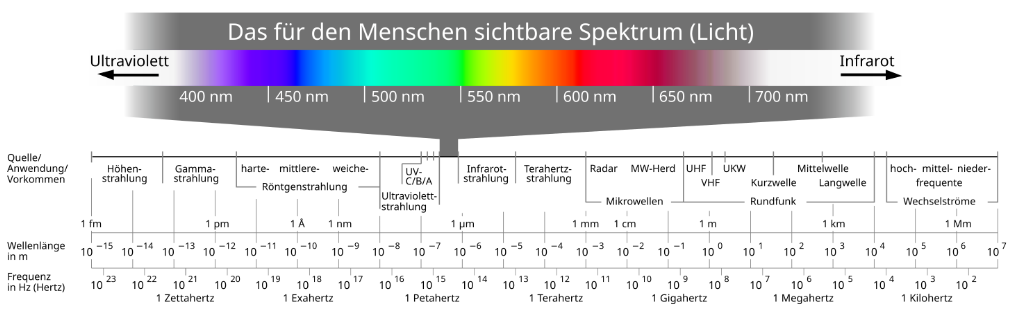
\includegraphics[width=\textwidth]{em_spektrum}
	\caption{Das Spektrum der elektromagnetischen Strahlung. Quelle: \href{https://de.wikipedia.org/wiki/Elektromagnetisches_Spektrum}{Wikipedia}.}
	\label{fig:1.1.3_1}
\end{figure}

Im Vakuum, da wo keine Materie vorhanden ist, kann die Wärmeübertragung weder durch Wärmeleitung noch durch Konvektion stattfinden. Nehmen wir ein Beispiel der Wärmeübertragung von der Sonne zur Erde an. Trotzt der Tatsache, dass der Raum zwischen der Erde und Sonne (fast) leer von Materie ist, findet die Wärmeübertragung von der Sonne auf die Erde statt. Es ist die \textit{Wärmestrahlung }, die für die Energieübertragung sorgt. Im Allgemeinen werden solche Prozesse durch das Konzept der elektromagnetischen Strahlung erklärt. Fakt ist, dass die elektromagnetische Strahlung kein Medium braucht um sich im Raum auszubreiten. Strahlung an sich kann mittels Wellen mathematisch beschrieben werden. Wellen schwingen, alles was schwingt hat eine Frequenz und kann daher in einem Frequenzspektrum eingeordnet werden. So ist die Wärmestrahlung nur ein Teil des gesamten elektromagnetischen Spektrums, wobei die UV-Strahlung, das sichtbare Spektrum und die Infrarot-Strahlung die Wärmestrahlung ausmachen (Abb.\ref{fig:1.1.3_1}). Tritt die Wärmestrahlung auf Materie, so wird sie absorbiert, wodurch sich die Materie aufwärmt oder gar erhitzt.

\section{Definition des Vorhabens}

\subsection{Das Problem}

Die vorangegangenen Überlegungen werden unten im Text herangezogen, um die theoretische Herangehensweise zum Problem der Wärmeausbreitung in Stoffen bereitzustellen ... bla bla ... was wird gemacht:

\begin{enumerate}
	\item Überlegungen, die aus physikalischen Gegebenheiten auf eine Gleichung Führen, im Kapitel \ref{cha:2}.
	\item Gleichung benennen, als Wärmegleichung, ev. Kapitel so und so.
	\item Mögliche Problemstellungen benennen, direkte und inverse ..., ev. Kapitel so und so
	\item Das Vorhaben benennen. Mit NN inverses Problem lösen, bla bla
	\item Die Struktur des Vorhabens schildern: FEM -> Lösung -> einige Werte der Lösung als Input für NN, , ev. Kapitel so und so
	\item Vergleich der Ergebnisse, ev. Kapitel so und so
\end{enumerate}
 Bla Bla ... somit ist das Ziel der vorliegenden Arbeit festgelegt worden

		\chapter{Wärmeleitungsproblem}
\label{cha:2}

\section{Herleitung der Wärmeleitungsgleichung}

Im Allgemeinen beschreibt die Wärmegleichung die Ausbreitung der Wärme in einem Medium. Das Medium kann beispielsweise ein räumlicher Gegenstand sein, zum Beispiel eine rechteckige Metallplatte. Man stelle sich vor, die gegebene Platte wird in der Mitte kurz erhitzt. Diesen Prozess kann man mithilfe einer Wärmebildkamera sichtbar machen.\\

Würde man diese Situation über einen Zeitraum beobachten, so würde man feststellen, dass die Temperatur in der Mitte der Platte sich über die gesamte Fläche verteilt. Und irgendwann kommt es zum Abkühlen, also zur Gleichverteilung der Temperatur in der Platte.\\

Der beschriebene Prozess kann mithilfe sogenannter Wärmeleitungsgleichung modelliert werden, die wir zunächst herleiten möchten.

\subsubsection*{Wärmeausbreitung}
Sei $\Omega \subset \R^{3}$ das Gebiet auf dem die Verteilung der Temperatur bestimmt werden soll.\footnote{\label{foot:1.2.1} Im Allgemeinen gilt $\Omega \subset \R^n$.} Die gesuchte Temperaturverteilung auf $\Omega$ in einem Zeitintervall $T = [t_0, t_1] \subset \R$ bezeichnen wir mit $u$. $u$ ordnet jedem Punkt $x \in \Omega$ zu jedem Zeitpunkt $t \in T$ eine Zahl $u(x, t) \in \R$ zu, also $u:\Omega \times T \longrightarrow \R$. Zusätzlich wollen wir die Bewegung der Wärme in $\Omega$ auffassen, es ist der Wärmefluss $j$. Für jeden Punkt $x \in \Omega$ zu jedem Zeitpunkt $t \in T$ gibt der Wärmefluss die Richtung in der die Wärmeenergie transportiert wird an, somit $j:\Omega \times T \longrightarrow \R^3$. Damit sind nötigen \textit{Variablen} für die Modellierung festgelegt.\\

Für die Herleitung der Gleichungen der Modellierung wird ein beliebiges Volumen $V \subset \Omega$ betrachtet. In einem homogenen Fall, also es gibt keine Wärmequellen, die in das Volumen $V$ die Wärmeenergie hinein oder heraus transportieren, würde man keinen Wärmestrom am Rand $dV$ detektieren, es gilt also

\begin{eqnarray}
	\int\limits_{\partial V} \langle j, v \rangle dS = 0.
	\label{equa:2.1_1}
\end{eqnarray}

Mit der Gleichung \ref{equa:2.1_1} wird der Strom $j$ in Richtung jeder Normalen $v$ am Rand $dV$ von $V$ aufsummiert (Abb.\ref{fig:1.2_1}). Und mit der Annahme, dass es keine Quellen gibt, erwarten wir eine 0 Summe.

%----------------------------------------------------------------------------------------
%	Beginn der Grafik
%----------------------------------------------------------------------------------------
\begin{figure}[!h]
	\centering
	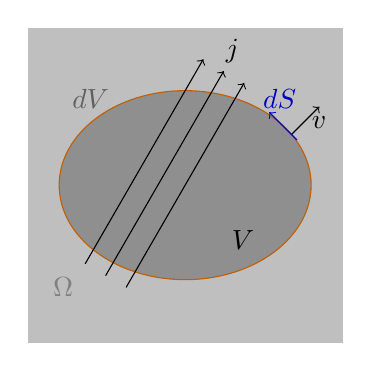
\begin{tikzpicture}
		
		
		\fill[lightgray] (0,0) ellipse (1.6cm and 1.2cm);	
		\draw[orange] (0,0) ellipse (1.6cm and 1.2cm);
		\draw[black](1, -0.7) node [left] {$V$};
		
		\draw [rotate=-30, xshift=-0.6cm, yshift=0.5cm, ->] [black] (0,-2) -- (0,1); % j
		\draw [rotate=-30, xshift=-0.3cm, yshift=0.5cm, ->] [black] (0,-2) -- (0,1); % j
		\draw [rotate=-30, xshift=0cm, yshift=0.5cm, ->] [black] (0,-2) -- (0,1); % j
		\draw [black] (0.6, 1.7)  node {$j$};	
		
		\draw [rotate=-45, xshift=0.5cm, yshift=1.41cm, ->] [black] (0,0) -- (0,0.5); % v
		\draw [black] (1.7,0.8)  node {$v$};	
		\draw [rotate=45, xshift=1.41cm, yshift=-0.6cm, ->] [blue] (0,0) -- (0,0.5); % dS
		\draw [blue] (1.2, 1.1)  node {$dS$};

		\draw [gray] (-1.2, 1.1)  node {$dV$};
						
		\fill[nearly transparent] (-2,-2) rectangle (2, 2); // Omega
		\draw[gray](-1.3, -1.3) node [left] {$\Omega$};
		
	\end{tikzpicture}	
	\caption{Schematische Darstellung der Gleichung \ref{equa:2.1_1}, mit $V$ das Volumen eine Mediums, $dV$ Rand (orange) von $V$, $j$ Der Wärmestrom durch $V$, $v \in \R^3$ Normalenvektor an $dV$ und $dS$ Tangente an $dV$.}
	\label{fig:1.2_1}
\end{figure}
%----------------------------------------------------------------------------------------
%	Ende der Grafik
%----------------------------------------------------------------------------------------

An dieser Stelle benötigen wie den \textit{Gauß'schen Satz} um das Oberflächenintegral \ref{equa:2.1_1} in ein Volumenintegral umzuschreiben.

\begin{Definition}
	\textbf{Der Gauß'sche Satz} \\
	Sei $V \subset	\R^n$ kompakt mit abschnittsweise glattem Rand $S = \partial V$, der Rand ist orientiert durch äußeres Normaleneinheitsvektorfeld $n$. Das Vektorfeld $F$ sei stetig differenzierbar auf einer offenen Menge $\Omega$ mit $V \in \Omega$. Dann gilt
	\begin{equation}
		\int\limits_{V} \langle \nabla,F \rangle dV = \int\limits_{\partial V} \langle F,n \rangle
		 dS.
		 \label{fig:2.1_2}
	\end{equation}
\end{Definition}

\begin{framed}
	\paragraph{Temporäres DenkZettel}

	\begin{itemize}
		\item[] \begin{Definition}
			Kompakte Menge \\
			$\R^n$ ist metrischer Raum. Wenn es für jede \textbf{offene Überdeckung} von $A \subset \R^n$, eine endliche Überdeckung gibt, also 
			\begin{eqnarray*}
				A \subset \bigcup\limits_{i \in I} U_i, \ \ \mbox{mit endlichem} \ I
			\end{eqnarray*} 			
		\end{Definition}
		\item[] \begin{Definition}
			Glatter Rand \\
			Sei $A \in \R^n$ kompakt, $A$ hat einen glatten Rand, wenn es zu jeden Punkt $x \in \partial A$ eine offene Umgebung $U \subseteq \R^n$ und $\psi : U \rightarrow \R, \ \psi \in C^n$ so gibt, dass 
			\begin{itemize}
				\item [(a)] $A \cap U = \{x \in U : \ \psi(x) \leq 0 \}$ 
				\item [(b)] $\forall x \in U : \psi'(x) \neq 0$
			\end{itemize}
			gilt.
		\end{Definition}		
	\end{itemize}
\end{framed}

Nun, der Gauß'sche Satz angewandt auf Gleichung \ref{equa:2.1_1} liefert folgendes Ergebnis
\begin{eqnarray}
	\int\limits_{V} \langle \nabla, j \rangle dx = \int\limits_{\partial V} \langle j, v \rangle dS = 0
	\label{fig:2.1_3}
\end{eqnarray}
Da, das Volumen $V$ nicht näher spezifiziert war, können wir aus \ref{fig:2.1_3} folgern, dass
{\color{red} Dahmen/Reusken: S.456, sinnvolle Argumentation nach dem Gaußschen Satz} \\

\begin{eqnarray}
	\langle \nabla, j \rangle = 0
	\label{equa:2.1_4}
\end{eqnarray}
auf ganz $\Omega$ gilt.

Als Nächstes, wollen wir herausfinden, wie $j$ und $u$ von einander abhängen. Eine einfache Modellannahme gibt uns das \textit{Fourier'sche Gesetz}:\footnote{\label{foot:1.2.2} J. B. Fourier, 1768-1830} 

\begin{center}
	\begin{minipage}{0.8\textwidth}
		\textit{Die Wärmeenergie strömt immer von Wärmeren Regionen zu den kälteren. Die Flussrate des Stroms ist proportional zum Temperaturgradienten.}
	\end{minipage}
\end{center}

Eine weitere Annahme für das Modell ist, dass jedes Material eine Eigenschaft hat, die Wärme auf seine Art und Weise zu leiten. Diese Eigenschaft nennt man die \textit{Wärmeleitfähigkeit} $a$. Sie ordnet jedem Punkt im Körper eine positive Zahl zu, also $a: \Omega \rightarrow \R_+$. Führen wir beide Überlegungen zusammen und erhalten 
\begin{eqnarray}
	j = -a \nabla u.
	\label{equa:2.1_5}
\end{eqnarray}
Einsetzen der Gleichung \ref{equa:2.1_5} in \ref{equa:2.1_4} führt uns zum folgenden Ausdruck
\begin{eqnarray}
	-\langle \nabla, a \nabla u \rangle = 0
	\label{equa:2.1_6}
\end{eqnarray}
Falls auf $\Omega$ noch zusätzliche Wärmequellen $f:\Omega \rightarrow \R$ vorhanden sind und die Wärmeverteilung \textit{instationär} ist, erhalten wir insgesamt folgende Gleichung \cite[S.5]{Schweizer18}
\begin{eqnarray}
	c \rho \ \partial_t u - \langle \nabla, a\nabla u \rangle = f
	\label{equa:2.1_7}
\end{eqnarray}

$c$ spezifische Wärmekapazität $[J/Kkg]$ \\
$\rho$ - Einheit $[kg/m^3]$ \\


{\color{red} Einschub über die Klassifikation der DGL} \\

Nie Gleichung \ref{equa:2.1_7} beschreibt ein abstraktes System. Die sogenannten Anfangs- und Randbedingungen würden eine mehr der Realität entsprechende Beschreibung des Wärmeleitungsproblems liefern. Jedes physikalische System besitzt zum Anfang der Messung oder der Beobachtung einen gewissen Anfangszustand $u_0$. Meistens wird die Zeit $t$ zu diesem Anfang auf den Wert 0 gesetzt, somit erhalten wir

\begin{eqnarray}
	u(x,0) = u_0(x), \ x \in \Omega
	\label{equa:2.1_8}
\end{eqnarray}

Die Randbedingungen geben die Temperaturverteilung $u$ am Rand $\partial \Omega$ des Gebiets $\Omega$ und können im Allgemeinen mit Sturm'schen Randbedingungen angegeben werden ({\color{red} oder gemischte Randbedingung?}):

\begin{eqnarray}
	u(x,t) = g(x, t), \ x \in \partial \Omega 
	%\dfrac{\partial}{\partial v} u(x,t) = \alpha(x)[u(x,t) - g(x)], 
	\label{equa:2.1_9}
\end{eqnarray}   

Nun kann man die Gleichungen \ref{equa:2.1_7}, \ref{equa:2.1_8} und \ref{equa:2.1_9} zusammen in einer Rand- und Anfangswertaufgabe (RAWP) der Wärmeleitung zusammenfassen, also:

\begin{Definition}
	\textbf{Rand- und Anfangswertaufgabe der Wärmeleitung} \\
	Sei $\Omega \subset	\R^3$ ein gebiet mit glattem Rand $\partial \Omega$, der Rand ist orientiert durch äußeres Normaleneinheitsvektorfeld $n$. So beschreibt das Modell
	\begin{equation}
		\begin{array}{llll}
			\partial_t u - \langle \nabla, a\nabla u \rangle & = & f & \\
			u(x,0) & = & u_0(x), & \ x \in \Omega \\
				u(x,t) & = & g(x, t), & \ x \in \partial \Omega
		\end{array}
		\label{equa:2.1_10}
	\end{equation}
	die Rand- und Anfangswertaufgabe der Wärmeleitung für alle $t \in T \subset \R$. 
	\label{def:2.1_4}
\end{Definition}

Das Ergebnis dieses Kapitels ist in der obigen Definition \ref{def:2.1_4} angegeben und wird als Grundmodell in folgenden Kapiteln dieser Arbeit vorausgesetzt.  

\subsection{Analytische Untersuchung der Wärmeleitungsgleichung}

Eventuell ...



%=====================================================================================================
% FORWARD PROBLEM 
%=====================================================================================================


\section{Vorwärtsproblem der Wärmeleitungsgleichung}

FEM als Grundlage des numerischen Ansatzes, warum und wieso ...

\subsection{Herleitung der Variationsformulierung der Wärmegleichung}

Die Wärmegleichung lautet:
\begin{equation}
	\partial_t u - \langle \nabla, a\nabla u \rangle  = f,
\end{equation}

und soll in die Variationsformulierung in schwacher Form umgeformt werden:
\begin{equation}
	\int_\Omega \frac{\partial u}{\partial t} v \, dx + \int_\Omega a(u) \nabla u \cdot \nabla v \, dx = \int_\Omega f v \, dx.
\end{equation}

Im Folgenden werden die Schritte zur Herleitung detailliert erläutert.

\subsection{Geometrie und Gitter definieren}
Die Geometrie und das Gitter definieren den Bereich $\Omega$, in dem die Gleichung gelöst wird. Das Gitter teilt diesen Bereich in kleine Unterbereiche (Finite Elemente) auf.

\subsubsection{Warum Geometrie und Gitter definieren?}
\begin{itemize}
	\item Die Methode der Finiten Elemente (FEM) basiert auf der Approximation der Lösung $u(x, y, t)$ auf einer diskreten Darstellung des Gebiets.
	\item Ein Gitter zerlegt $\Omega$ in einfachere Formen (z. B. Dreiecke oder Vierecke). Innerhalb jedes Elements wird die Lösung lokal approximiert.
\end{itemize}

\subsubsection{Beispiel für ein rechteckiges Gebiet}
\begin{equation}
	\Omega = \{(x, y) \mid 0 \leq x \leq L_x, \, 0 \leq y \leq L_y\}.
\end{equation}
Dieses Gebiet könnte mit Dreiecken oder Rechtecken diskretisiert werden.

\subsection{Funktionsräume definieren}
Ein Funktionsraum beschreibt, wie die Lösung $u$ und die Testfunktionen $v$ innerhalb der Finiten Elemente dargestellt werden.

\subsubsection{Was sind $P_1$- und $P_2$-Elemente?}
\begin{itemize}
	\item $P_1$: Lineare Basisfunktionen – $u$ wird innerhalb eines Elements als lineares Polynom approximiert.
	\item $P_2$: Quadratische Basisfunktionen – $u$ wird innerhalb eines Elements als quadratisches Polynom approximiert.
\end{itemize}
Diese Basisfunktionen gewährleisten, dass $u$ über das gesamte Gebiet hinweg stetig ist.

\subsubsection{Warum Funktionsräume definieren?}
Die Funktionsräume sorgen dafür, dass die approximierte Lösung $u$ und die Testfunktionen $v$ die notwendigen Kontinuitäts- und Randbedingungen der PDE erfüllen.

\subsection{Variationsformulierung herleiten}
Die Variationsformulierung (schwache Form) wird durch Multiplikation der PDE mit einer Testfunktion $v$ und Integration über das Gebiet $\Omega$ hergeleitet. Dieser Schritt erlaubt es, auch Lösungen $u$ zu berücksichtigen, die möglicherweise nicht überall differenzierbar sind.

\subsubsection{Herleitung der schwachen Form}
\begin{enumerate}
	\item \textbf{Starte mit der PDE:}
	\begin{equation}
		\frac{\partial u}{\partial t} - \nabla \cdot \big(a(u) \nabla u\big) = f.
	\end{equation}
	
	\item \textbf{Multipliziere mit einer Testfunktion $v$:} Multipliziere beide Seiten mit einer glatten Testfunktion $v \in V$, wobei $V$ der Raum der zulässigen Testfunktionen ist:
	\begin{equation}
		v \left(\frac{\partial u}{\partial t} - \nabla \cdot \big(a(u) \nabla u\big)\right) = v f.
	\end{equation}
	
	\item \textbf{Integriere über $\Omega$:}
	\begin{equation}
		\int_\Omega v \frac{\partial u}{\partial t} \, dx - \int_\Omega v \nabla \cdot \big(a(u) \nabla u\big) \, dx = \int_\Omega v f \, dx.
	\end{equation}
	
	\item \textbf{Wende den Divergenzsatz an:} Für den zweiten Term wende den Divergenzsatz an, um das Volumenintegral in ein Oberflächenintegral umzuwandeln:
	\begin{equation}
		\int_\Omega v \nabla \cdot \big(a(u) \nabla u\big) \, dx = \int_{\partial \Omega} v \big(a(u) \nabla u \cdot \mathbf{n}\big) \, dS - \int_\Omega \nabla v \cdot \big(a(u) \nabla u\big) \, dx.
	\end{equation}
	Hier ist $\partial \Omega$ der Rand des Gebiets und $\mathbf{n}$ der nach außen gerichtete Normalenvektor.
	
	\item \textbf{Vereinfachung bei homogenen Randbedingungen:} Unter der Annahme homogener Dirichlet-Randbedingungen ($u = 0$ auf dem Rand) verschwindet der Oberflächenterm:
	\begin{equation}
		\int_\Omega v \nabla \cdot \big(a(u) \nabla u\big) \, dx = -\int_\Omega \nabla v \cdot \big(a(u) \nabla u\big) \, dx.
	\end{equation}
	
	\item \textbf{Kombiniere die Terme:} Substituiere zurück in die Gleichung. Die schwache Form lautet:
	\begin{equation}
		\int_\Omega v \frac{\partial u}{\partial t} \, dx + \int_\Omega a(u) \nabla u \cdot \nabla v \, dx = \int_\Omega v f \, dx.
	\end{equation}
\end{enumerate}

\subsection{Zeitdiskretisierung}
Die Zeitdiskretisierung ist notwendig, um die Lösung schrittweise für diskrete Zeitpunkte zu berechnen.

\subsubsection{Warum Zeitdiskretisierung?}
\begin{itemize}
	\item Der Term $\frac{\partial u}{\partial t}$ ist eine partielle Ableitung nach der Zeit. FEM-Frameworks lösen jedoch räumliche Ableitungen.
	\item Die Zeitdiskretisierung ersetzt $\frac{\partial u}{\partial t}$ durch eine algebraische Differenz.
\end{itemize}

\subsection{Backward-Euler-Verfahren}
Das Backward-Euler-Verfahren approximiert $\frac{\partial u}{\partial t}$ zum Zeitpunkt $t_{n+1}$:
\begin{equation}
	\frac{\partial u}{\partial t} \approx \frac{u^{n+1} - u^n}{\Delta t}.
\end{equation}
Setze dies in die schwache Form ein:
\begin{equation}
	\int_\Omega \frac{u^{n+1} - u^n}{\Delta t} v \, dx + \int_\Omega a(u^{n+1}) \nabla u^{n+1} \cdot \nabla v \, dx = \int_\Omega v f^{n+1} \, dx.
\end{equation}
Dies führt zu einem System von Gleichungen, das für jeden Zeitschritt numerisch gelöst werden kann.

\subsection{Schlüsselkonzepte}
\begin{itemize}
	\item \textbf{Testfunktion $v$:} Eine Testfunktion $v$ gehört demselben Funktionsraum wie $u$ und stellt sicher, dass die schwache Form für alle zulässigen Lösungen $u$ gilt.
	\item \textbf{Warum schwache Form?}
	\begin{itemize}
		\item Die schwache Form ermöglicht es, die PDE für Funktionen $u$ zu lösen, die möglicherweise nicht überall differenzierbar sind (z. B. wenn $\nabla u$ nicht existiert).
		\item Die Integration durch Teile verschiebt die Ableitung von $u$ auf die Testfunktion $v$, die als glatt angenommen wird.
	\end{itemize}
\end{itemize}


....


%=====================================================================================================
% INVERSE PROBLEM 
%=====================================================================================================

\section{Inverses Problem der Wärmeleitung}

{\color{red}Inverses Problem aus der Praktischen Sicht, also $u(x,y,t)$ wird gemessen und $a(x,y)$ dann bestimmt ...} \\\\


Betrachten wir das Problem aus der Definition \ref{def:2.1_4}, insbesondere die Wärmeleitfähigkeit $a$. In vielen praktischen Problemstellungen hängt die Wärmeleitfähigkeit direkt von der Temperatur $u(x,t)$ ab (\cite[S. 506]{Handrock-Meyer88}), also gilt $a:\R \longrightarrow \R$.

Die DGL aus der Definition \ref{def:2.1_4} bleibt bei dieser Betrachtung dieselbe, jedoch wird $a$ jetzt explizit als Funktion von $u$ betrachtet, also:

\begin{equation}
	\frac{\partial u}{\partial t} - \nabla \cdot \big(a(u) \nabla u\big) = f
	\label{equa:2.1_11}
\end{equation}

Um $a(u)$ zu isolieren, können wir folgendermaßen vorgehen:
\begin{enumerate}
	\item Schreibe die Gleichung um, sodass der diffusive Term isoliert wird:
	\[
	-\nabla \cdot \big(a(u) \nabla u\big) = f - \frac{\partial u}{\partial t}.
	\]
	
	\item Verwende die Produktregel für den diffusen Term:
	\[
	-\nabla \cdot \big(a(u) \nabla u\big) = -a(u) \nabla^2 u - \nabla a(u) \cdot \nabla u = -a(u) \Delta u - \nabla a(u) \cdot \nabla u.
	\]
	
	\item Wenn wir annehmen, dass $a(u)$ nur von $u$ abhängt (keine explizite Abhängigkeit von $x, y$), vereinfacht sich der Gradienten-Term:
	\[
	\nabla a(u) = \frac{da(u)}{du} \nabla u.
	\]
	
	\item Setze dies in die Gleichung ein:
	\[
	-a(u) \nabla^2 u - \frac{da(u)}{du} (\nabla u \cdot \nabla u) = f - \frac{\partial u}{\partial t}.
	\]
	
	\item Gruppiere die Terme, um $a(u)$ zu isolieren:
	\[
	a(u) = -\frac{1}{\nabla^2 u}\Big(f - \frac{\partial u}{\partial t} + \frac{da(u)}{du} (\nabla u \cdot \nabla u)\Big).
	\]
\end{enumerate}


die Wärmeleitungsgleichung im Gebiet $\Omega \subset \R^2$ mit zeitlicher Dimension $t \in T \subset \R$:
\[
\frac{\partial u}{\partial t} - \nabla \cdot (a \nabla u) = f,
\]
ergänzt durch Anfangsbedingungen
\[
u(x,0) = u_0(x,y) \quad \text{für } x \in \Omega,
\]
und Dirichlet-Randbedingungen
\[
u(x,t) = g(x,t) \quad \text{für } x \in \partial \Omega, \, t \in (0,T].
\]

Das inverse Problem besteht darin, $a(u)$ zu finden, sodass die Differentialgleichung und die Randbedingungen erfüllt werden, wenn $u(x,t)$ und $f(x,t)$ bekannt sind.

\subsection{Existenz und Eindeutigkeit}

\subsubsection{Satz 1: Existenz der Lösung}

Sei $u(x,y,t)$ eine hinreichend glatte Lösung der Wärmeleitungsgleichung und $f(x,y,t)$ sowie $u_0(x,y)$ bekannt. Dann existiert unter geeigneten Regularitätsvoraussetzungen an die Daten eine Funktion $a(x,y)$, die das inverse Problem löst.

\paragraph{Beweisidee:}
\begin{enumerate}
	\item Schreibe die Wärmeleitungsgleichung in schwacher Form:
	\[
	\int_{\Omega} \left( \frac{\partial u}{\partial t} v + a(x,y) \nabla u \cdot \nabla v \right) \, d\Omega = \int_{\Omega} f(x,y,t) v \, d\Omega,
	\]
	für alle Testfunktionen $v \in H^1(\Omega)$.
	\item Die Lösung $a(x,y)$ ergibt sich aus der schwachen Form, indem $u$ und $\nabla u$ durch die Messdaten approximiert werden. Standardresultate aus der Variationsrechnung garantieren die Existenz von $a(x,y)$.
\end{enumerate}

\subsubsection{Satz 2: Eindeutigkeit der Lösung}

Seien $u(x,y,t)$ und $f(x,y,t)$ eindeutig gegeben, und sei $u$ hinreichend differenzierbar. Dann ist $a(x,y)$ eindeutig bestimmt, wenn $\nabla u \neq 0$ in $\Omega$.

\paragraph{Beweis:} Nehmen wir an, es existieren zwei Funktionen $a_1(x,y)$ und $a_2(x,y)$, die das inverse Problem lösen. Dann gilt:
\[
\frac{\partial u}{\partial t} - \nabla \cdot (a_1 \nabla u) = f = \frac{\partial u}{\partial t} - \nabla \cdot (a_2 \nabla u).
\]
Durch Subtraktion erhalten wir:
\[
\nabla \cdot \left( (a_1 - a_2) \nabla u \right) = 0.
\]
Da $\nabla u \neq 0$, folgt aus der Divergenzfreiheit, dass $a_1 = a_2$ fast überall in $\Omega$. Dies zeigt die Eindeutigkeit.

\subsection{Stabilität}

\subsubsection{Satz 3: Stabilität der Lösung}

Sei $u_{\text{obs}}(x,y,t)$ eine Rauschbehaftung der exakten Lösung $u(x,y,t)$ mit einem maximalen Fehler $\epsilon > 0$, d. h.
\[
\| u_{\text{obs}} - u \|_{L^2} \leq \epsilon.
\]
Dann existiert eine Konstante $C > 0$, sodass der Fehler in $a(x,y)$ beschränkt ist durch
\[
\| a_{\text{obs}} - a \|_{L^2} \leq C \epsilon.
\]

\paragraph{Beweisidee:}
\begin{enumerate}
	\item Schreibe die Wärmeleitungsgleichung als Operatorgleichung:
	\[
	\mathcal{A}(a) = f,
	\]
	wobei $\mathcal{A}(a) = \frac{\partial u}{\partial t} - \nabla \cdot (a \nabla u)$.
	\item Zeige, dass der Operator $\mathcal{A}$ stetig und Lipschitz-stetig bezüglich $a$ ist.
	\item Wende den Satz von Lax-Milgram oder perturbative Stabilitätsresultate an, um die beschränkte Fehlerfortpflanzung von $u$ auf $a$ zu zeigen.
\end{enumerate}

\subsection{Regularisierung des inversen Problems}

Da inverse Probleme oft schlecht gestellt sind, d. h. kleine Fehler in den Daten können zu großen Abweichungen in der Lösung führen, wird eine Regularisierung benötigt.

\subsubsection{Definition (Regularisierte Zielfunktion)}

Das inverse Problem wird als Minimierung einer modifizierten Zielfunktion formuliert:
\[
J(a) = \int_{\Omega} \int_0^T \left| \frac{\partial u}{\partial t} - \nabla \cdot (a \nabla u) - f \right|^2 \, dt \, d\Omega + \lambda R(a),
\]
wobei $R(a)$ eine Regularisierungsfunktion ist, typischerweise:
\begin{itemize}
	\item $R(a) = \| a \|_{H^1(\Omega)}^2$ (Tikhonov-Regularisierung) oder
	\item $R(a) = \int_{\Omega} |\nabla a|^2 \, d\Omega$ (Glattheitsregularisierung).
\end{itemize}

\subsubsection{Satz 4: Existenz der regularisierten Lösung}

Sei $J(a)$ schwach unterer-halbstetig und sei $R(a)$ strikt konvex. Dann existiert mindestens eine minimierende Funktion $a \in H^1(\Omega)$, die das reguläre inverse Problem löst.

\paragraph{Beweis:}
\begin{enumerate}
	\item Schwache Halbstetigkeit und kompakte Einbettungen von Sobolev-Räumen garantieren die Existenz einer minimierenden Funktion.
	\item Die Konvexität von $R(a)$ sorgt dafür, dass die Lösung eindeutig ist.
\end{enumerate} 




\section{Ansatz des maschinellen Lernens}

Traditionelle numerische Methoden wie Finite-Differenzen oder Finite-Elemente sind häufig mit hohen Rechenkosten verbunden. Eine vielversprechende Methode zur Lösung dieser Probleme stellen Physics-Informed Neural Networks (PINNs) dar, die maschinelles Lernen mit physikalischen Modellen kombinieren.

Dieses Kapitel beginnt mit einer detaillierten Einführung in die Grundlagen des statistischen Lernens, das eine mathematische Grundlage für maschinelles Lernen bildet. Anschließend wird die Theorie von PINNs eingeführt und detailliert ausgebaut.

\section{Statistisches Lernen: Grundlagen}

\subsection{Definition des statistischen Lernens}
Das Ziel des statistischen Lernens ist es, eine Abbildung $f : X \to Y$ zu finden, die die zugrunde liegende Verteilung der Daten möglichst gut approximiert. Hierbei sind $X$ der Raum der Eingabedaten und $Y$ der Raum der Zielgrößen (z. B. Labels). Formal lässt sich das Problem des Lernens als Minimierung eines Risikos beschreiben.

Sei $(x_i, y_i)$ eine i.i.d. Stichprobe aus einer unbekannten gemeinsamen Verteilung $P(x, y)$. Ziel ist es, ein Modell $f$ aus einem Hypothesenraum $\mathcal{F}$ zu finden, das die zugehörige Verlustfunktion minimiert. Das Risiko-Funktional ist gegeben durch:
\[
R(f) = \mathbb{E}_{(x, y) \sim P}[L(y, f(x))],
\]
wobei $L : Y \times Y \to \mathbb{R}^+$ eine Verlustfunktion ist. Die Erwartung wird hierbei über die wahre Datenverteilung $P(x, y)$ genommen.

Da jedoch die wahre Verteilung $P(x, y)$ nicht bekannt ist, wird das Risiko durch den empirischen Risikofunktional approximiert:
\[
R_n(f) = \frac{1}{n} \sum_{i=1}^n L(y_i, f(x_i)),
\]
wobei $(x_i, y_i)$ die beobachteten Trainingsdaten sind.

Die Zielsetzung des Lernens besteht also darin, den Schätzer $f$ zu finden, der das Risiko minimiert:
\[
\hat{f} = \arg \min_{f \in \mathcal{F}} R_n(f).
\]

Eine zentrale Annahme des statistischen Lernens ist, dass das Modell $f$ generalisierbar ist, d. h., es kann auf neue, unbekannte Daten angewendet werden.

\subsection{Lineare Modelle und Regression}
Eine der einfachsten und am häufigsten verwendeten Klassen von Modellen im statistischen Lernen sind lineare Modelle. Das grundlegende lineare Modell wird durch
\[
f(x) = w^\top x + b
\]
gegeben, wobei $w \in \mathbb{R}^d$ der Gewichtungsvektor und $b \in \mathbb{R}$ der Bias-Term sind. In der linearen Regression wird $f(x)$ so gewählt, dass der Fehler zwischen den Vorhersagen $f(x_i)$ und den tatsächlichen Werten $y_i$ minimiert wird.

Die Verlustfunktion ist hierbei oft die quadratische Verlustfunktion:
\[
L(y, f(x)) = \|y - f(x)\|^2.
\]

Um die Parameter $w$ und $b$ zu optimieren, minimiert man das empirische Risiko:
\[
R_n(w, b) = \frac{1}{n} \sum_{i=1}^n \|y_i - (w^\top x_i + b)\|^2.
\]

Durch Anwendung der Methode der kleinsten Quadrate ergibt sich eine Lösung für $w$ und $b$, die durch die Normalengleichung beschrieben wird:
\[
\hat{w}, \hat{b} = \arg \min_{w, b} R_n(w, b).
\]

Die Lösung dieser Gleichung lässt sich durch:
\[
\hat{w} = (X^\top X)^{-1} X^\top y
\]
für $w$ (wobei $X$ die Designmatrix ist) und $\hat{b}$ durch den Mittelwert der Zielwerte berechnen.

\subsection{Nichtlineare Modelle und neuronale Netze}
Da lineare Modelle für viele Probleme nicht ausreichend sind, hat sich die Nutzung nichtlinearer Modelle als Standard etabliert. Ein prominentes nichtlineares Modell ist das neuronale Netz. Ein neuronales Netz ist eine Verknüpfung von linearen Transformationen und nichtlinearen Aktivierungsfunktionen. Ein einfaches Feedforward-Netzwerk besteht aus mehreren Schichten, wobei die Funktion eines neuronalen Netzes durch
\[
f(x) = \sigma\big(W^{(L)} \sigma(W^{(L-1)} \dots \sigma(W^{(1)} x + b^{(1)}) \dots + b^{(L-1)}) + b^{(L)}\big)
\]
gegeben ist. Hierbei sind $W^{(l)}$ die Gewichtsmatrizen und $b^{(l)}$ die Bias-Vektoren der $l$-ten Schicht, und $\sigma$ ist eine nichtlineare Aktivierungsfunktion wie ReLU oder Sigmoid.

Neuronale Netze werden häufig mit Gradientenabstieg optimiert, indem die Kreuzentropie-Verlustfunktion oder die Mean Squared Error (MSE)-Verlustfunktion minimiert wird:
\[
L(y, f(x)) = \|y - f(x)\|^2.
\]

Die Optimierung erfolgt durch Rückpropagation und den Gradientenabstiegsalgorithmus.

Hier ein kurzer Exkurs zum Prinzip der Werteapproximation mit NN.


\subsection{Das Prinzip der neuronalen Netze (NN)}

\subsubsection{Vorwärtsdurchlauf (Forward Pass)}

Ein neuronales Netz besteht aus \textbf{Schichten} von Neuronen, die jeweils eine affine Transformation gefolgt von einer nichtlinearen Aktivierungsfunktion anwenden.

\begin{itemize}
	\item \textbf{Eingangsvektor}: $ x \in \mathbb{R}^d $ (mit Eingabedimension $ d $)
	\item \textbf{Gewichte}: $ W^{(l)} \in \mathbb{R}^{n_{l} \times n_{l-1}} $ (Anzahl der Neuronen pro Schicht $ n_l $)
	\item \textbf{Bias}: $ b^{(l)} \in \mathbb{R}^{n_l} $
	\item \textbf{Aktivierungsfunktion}: $ \sigma: \mathbb{R} \to \mathbb{R} $
\end{itemize}

Die Transformation einer Schicht:
\begin{equation}
	z^{(l)} = W^{(l)} a^{(l-1)} + b^{(l)}
\end{equation}

Die Aktivierung:
\begin{equation}
	a^{(l)} = \sigma(z^{(l)})
\end{equation}

Gängige Aktivierungsfunktionen:
\begin{itemize}
	\item \textbf{ReLU}: $ \sigma(x) = \max(0, x) $
	\item \textbf{Sigmoid}: $ \sigma(x) = \frac{1}{1 + e^{-x}} $
	\item \textbf{Tanh}: $ \sigma(x) = \frac{e^x - e^{-x}}{e^x + e^{-x}} $
\end{itemize}

Der endgültige Output nach $ L $ Schichten:
\begin{equation}
	\hat{y} = a^{(L)}
\end{equation}

Nach der Berechnung des Outputs erfolgt dessen Fehleranalyse.

\subsubsection{Fehlermessung (Loss-Funktion)}

Die Loss-Funktion misst den Unterschied zwischen Vorhersage und wahrem Wert. Hier ein Paar Ansätze für die Loss-Funktionen: \\

\textbf{Mittlerer quadratischer Fehler (MSE)}
\begin{equation}
	\mathcal{L}(\theta) = \frac{1}{N} \sum_{i=1}^{N} (y_i - \hat{y}_i)^2
\end{equation}

\subsubsection{Backpropagation (Gradientenberechnung)}

Backpropagation nutzt die Kettenregel der Ableitung, um die Änderung des Fehlers bezüglich der Gewichte zu berechnen.

\begin{equation}
	\frac{\partial \mathcal{L}}{\partial a^{(L)}} = -\frac{2}{N} (y - \hat{y})
\end{equation}

Für das letzte Layer gilt:

\begin{equation} 
	\dfrac{\partial \mathcal{L}}{\partial W^{(L)}} = \delta^{(L)}  a^{(L-1)T}
\end{equation}

mit
\begin{equation}
	\delta^{(L)} = \frac{\partial \mathcal{L}}{\partial a^{(L)}} \cdot \sigma'(z^{(L)})
\end{equation}

Rekursiv für vorherige Schichten:
\begin{equation}
	\delta^{(l)} = (W^{(l+1)})^T \delta^{(l+1)} \cdot \sigma'(z^{(l)})
\end{equation}

\subsubsection{Gradientenabstieg (Gewichtsaktualisierung)}

\begin{equation}
	W^{(l)} = W^{(l)} - \eta \frac{\partial \mathcal{L}}{\partial W^{(l)}}
\end{equation}

mit der Lernrate $ \eta $.

\subsection{Optimierte Gradienten-Methoden}

\subsubsection{Stochastischer Gradientenabstieg (SGD)}
\begin{equation}
	W = W - \eta \nabla \mathcal{L}(W, x_i)
\end{equation}

\subsubsection{Adam Optimizer}
\begin{align}
	m_t &= \beta_1 m_{t-1} + (1 - \beta_1) g_t \\
	v_t &= \beta_2 v_{t-1} + (1 - \beta_2) g_t^2 \\
	\hat{m_t} &= \frac{m_t}{1 - \beta_1^t}, \quad \hat{v_t} = \frac{v_t}{1 - \beta_2^t} \\
	W &= W - \eta \frac{\hat{m_t}}{\sqrt{\hat{v_t}} + \epsilon}
\end{align}

\section{Einführung in Physics-Informed Neural Networks}

\subsection{Motivation für PINNs}
In vielen physikalischen Problemen, wie der Wärmeleitungsgleichung, sind die zugrunde liegenden physikalischen Gesetze bekannt und können als Randbedingungen und PDEs formuliert werden. In vielen praktischen Anwendungen ist jedoch das inverse Problem von Interesse: Man möchte aus Messdaten, die an den Randbedingungen oder an einem Teil des Systems erfasst werden, die vollständige Lösung der PDE rekonstruieren.


\subsection{Theorie für das inverse Problem der Wärmeleitung}

\subsubsection{Das zugrunde liegende Problem}

Die modifizierte Wärmeleitungsgleichung lautet:
\[
\frac{\partial u}{\partial t} - \nabla \cdot \big(a(u) \nabla u\big) = f(x, y, t),
\]
wobei:
\begin{itemize}
	\item \(u(x, y, t)\) die Temperaturverteilung ist,
	\item \(a(u)\) eine unbekannte temperaturabhängige Wärmeleitfähigkeit darstellt,
	\item \(f(x, y, t)\) eine unbekannte Wärmequelle ist.
\end{itemize}

Das inverse Problem besteht darin, die Funktionen \(a(u)\) und \(f(x, y, t)\) basierend auf Messungen der Temperatur \(u_\text{obs}(x, y, t)\) zu rekonstruieren.

\subsection{Formulierung als Variationsproblem}

Für das inverse Problem wird das Modell in ein Optimierungsproblem überführt. Die Zielfunktion besteht aus einem Datenanpassungsterm und physikalischen Residuen:
\[
\mathcal{J}(u, a, f) = \mathcal{J}_\text{Data}(u) + \mathcal{J}_\text{PDE}(u, a, f),
\]
wobei:
\begin{itemize}
	\item \textbf{Datenanpassung:}
	\[
	\mathcal{J}_\text{Data}(u) = \frac{1}{2} \int_0^T \int_\Omega \big(u(x, y, t) - u_\text{obs}(x, y, t)\big)^2 \, \mathrm{d}\Omega \, \mathrm{d}t,
	\]
	\item \textbf{PDE-Residuum:}
	\[
	\mathcal{J}_\text{PDE}(u, a, f) = \frac{1}{2} \int_0^T \int_\Omega \bigg(\frac{\partial u}{\partial t} - \nabla \cdot \big(a(u) \nabla u\big) - f(x, y, t)\bigg)^2 \, \mathrm{d}\Omega \, \mathrm{d}t.
	\]
\end{itemize}

Zur Stabilisierung wird eine Regularisierung hinzugefügt:
\[
\mathcal{J}_\text{Reg}(a, f) = \alpha \|a(u)\|_{H^1}^2 + \beta \|f(x, y, t)\|_{L^2}^2,
\]
wobei \(\alpha, \beta > 0\) Regularisierungsparameter sind.

Die kombinierte Zielfunktion lautet:
\[
\mathcal{J}(u, a, f) = \mathcal{J}_\text{Data}(u) + \mathcal{J}_\text{PDE}(u, a, f) + \mathcal{J}_\text{Reg}(a, f).
\]

\subsection{Existenz und Eindeutigkeit}

\textbf{Satz 1 (Existenz):}  
Unter der Annahme, dass die Beobachtungsdaten \(u_\text{obs}\) ausreichend regelmäßig sind (\(u_\text{obs} \in H^1(\Omega \times (0, T))\)), existiert eine Lösung \((u, a, f)\) des Optimierungsproblems.

\textit{Beweis (Skizze):}
\begin{enumerate}
	\item Zeige, dass die Zielfunktion \(\mathcal{J}\) nach unten beschränkt ist.
	\item Zeige, dass die Menge der zulässigen Parameter \((u, a, f)\) schwach kompakt ist.
	\item Wende den Satz von Weierstraß auf das minimierende Funktional an.
\end{enumerate}

\textbf{Bemerkung:}  
Die Eindeutigkeit ist im Allgemeinen nicht garantiert, da das Problem schlecht gestellt ist (mehrere Kombinationen von \(a(u)\) und \(f(x, y, t)\) können dieselben Messdaten erklären). Regularisierungen wie \(H^1\)- und \(L^2\)-Normen tragen dazu bei, die Lösung zu stabilisieren.

\subsection{PINNs für das inverse Problem}

Ein Physics-Informed Neural Network (PINN) wird verwendet, um sowohl die Temperatur \(u(x, y, t)\) als auch die unbekannten Funktionen \(a(u)\) und \(f(x, y, t)\) zu approximieren. Die neuronalen Netze sind wie folgt definiert:
\begin{itemize}
	\item \(u(x, y, t; \theta_u)\): Neuronales Netz zur Approximation der Temperatur,
	\item \(a(u; \theta_a)\): Neuronales Netz für die Wärmeleitfähigkeit,
	\item \(f(x, y, t; \theta_f)\): Neuronales Netz für die Wärmequelle.
\end{itemize}

Die Verlustfunktion des PINN-Modells kombiniert mehrere Terme:
\[
\mathcal{L} = \mathcal{L}_\text{Data} + ( \mathcal{L}_\text{PDE} + \mathcal{L}_\text{BC} + \mathcal{L}_\text{IC} ) + \mathcal{L}_\text{Reg}.
\]
\begin{itemize}
	\item \textbf{Datenanpassung:}
	\[
	\mathcal{L}_\text{Data} = \frac{1}{N_\text{obs}} \sum_{i=1}^{N_\text{obs}} \big(u(x_i, y_i, t_i; \theta_u) - u_\text{obs}(x_i, y_i, t_i)\big)^2,
	\]
	\item \textbf{PDE-Residuum:}
	\[
	\mathcal{L}_\text{PDE} = \frac{1}{N_\text{PDE}} \sum_{i=1}^{N_\text{PDE}} \bigg(\frac{\partial u}{\partial t} - \nabla \cdot \big(a(u; \theta_a) \nabla u\big) - f(x, y, t; \theta_f)\bigg)^2,
	\]
	\item \textbf{Regularisierung:}
	\[
	\mathcal{L}_\text{Reg} = \alpha \|\nabla_\theta a(u; \theta_a)\|^2 + \beta \|\nabla_\theta f(x, y, t; \theta_f)\|^2.
	\]
\end{itemize}

Das PINN wird durch Minimierung der Verlustfunktion trainiert:
\[
\theta_u^*, \theta_a^*, \theta_f^* = \arg \min_{\theta_u, \theta_a, \theta_f} \mathcal{L}.
\]

\subsection{Eigenschaften und Herausforderungen}

\begin{itemize}
	\item \textbf{Kopplung von \(a(u)\) und \(f(x, y, t)\):}  
	Die Rekonstruktion von \(a(u)\) ist nichtlinear gekoppelt mit der Lösung \(u(x, y, t)\), da \(a\) explizit von \(u\) abhängt. Diese Nichtlinearität führt zu Herausforderungen in der Konvergenz der Optimierung.
	\item \textbf{Ill-posedness:}  
	Das inverse Problem bleibt empfindlich gegenüber Rauschen in den Beobachtungsdaten. Regularisierungen und sorgfältig gewählte Netzarchitekturen sind entscheidend.
	\item \textbf{Einschränkungen:}  
	Die Lösungsgüte hängt stark von der Verfügbarkeit hochauflösender Messdaten \(u_\text{obs}\) ab, insbesondere für stark heterogene Materialien oder schnell variierende Wärmequellen.
\end{itemize}


		\chapter{Auswertung der praktischen Arbeit}
\label{cha:3}

\section{Architektur der Implementierung}

\section{Diskussion der Ergebnisse}


\section{Ausblick}


		% Tämporer zum abschauen
		\chapter*{Vorlage der BA}

\section*{Das des Computertomographen}

Das Wort Tomographie setzt sich aus zwei dem Altgriechischen entstammten Wörtern zusammen. $\tau o\mu\eta$ [\textit{tome}], bedeutet Schnitt und $\gamma\rho\alpha\varphi\varepsilon\iota\nu$ [\textit{graphien}] bezeichnet Schreiben. Zusammengefasst zu einem Wort \textit{Tomographie} kann es als Schnittbild eines Objekts verstanden werden. 

Die CT ist ein bildgebendes Verfahren, das in der medizinischen Radiologie und in der Materialforschung eingesetzt wird. Die Technologie des Verfahrens erlaubt eine zerstörungsfreie Materialuntersuchung. Das ausschlaggebende Wort ist hier \textit{zerstörungsfrei}, damit ist die Untersuchung des inneren Aufbaus eines Objekts, ohne es zu öffnen, gemeint. 
%----------------------------------------------------------------------------------------
%	Beginn der Grafik
%----------------------------------------------------------------------------------------
\begin{figure}[!h]
	\centering
	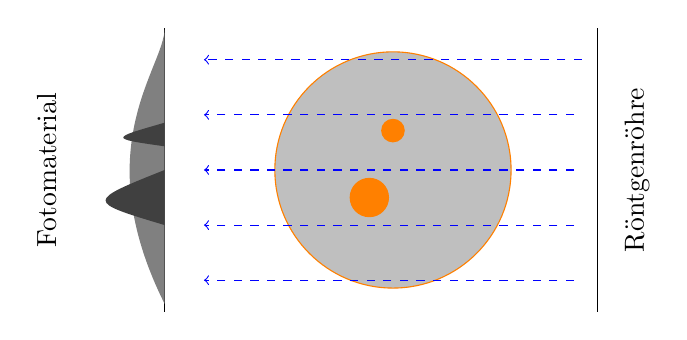
\begin{tikzpicture}[domain=3:3]  
	
	\fill[lightgray] (0.9,0.7) circle (1.5cm);
	
	\draw [rotate=90, yshift=2cm, -](-1.1,0) -- (2.5,0); % s-Achse
	
	\draw  (-0.5, 0.7) node [rotate=90, yshift=3cm] {Fotomaterial};
	
	\fill[gray] [rotate=90, yshift=2cm] (-1,0) .. controls (1,1) and (2,0) .. (2.5,0);
	\fill[darkgray] [rotate=90, yshift=2cm] (0,0) .. controls (0.3,1)  .. (0.7,0);
	\fill[darkgray] [rotate=90, yshift=2cm] (1,0) .. controls (1.1,0.7)  .. (1.3,0);
	
	\draw[orange] (0.9,0.7) circle (1.5cm);
	\fill[orange] (0.9,  1.2) circle (.15cm);
	\fill[orange] (0.6, 0.35) circle (.25cm);
	
	\draw [rotate=90, dashed, ->] [blue] (0,-3.2) -- (0,1.5); % strahl
	\draw [rotate=90, xshift=-0.7cm, dashed, ->] [blue] (0,-3.2) -- (0,1.5); % strahl
	\draw [rotate=90, xshift=0.7cm, dashed, ->] [blue] (0,-3.2) -- (0,1.5); % strahl
	\draw [rotate=90, xshift=1.4cm, dashed, ->] [blue] (0,-3.2) -- (0,1.5); % strahl
	\draw [rotate=90, xshift=2.1cm, dashed, ->] [blue] (0,-3.3) -- (0,1.5); % strahl
	
	\draw [rotate=90, yshift=-3.5cm, -](-1.1,0) -- (2.5,0); % Sensor-Achse
	\draw  (3, 0.7) node [rotate=90, yshift=-1cm, -] {Röntgenröhre};
	
	\begin{scope}[xshift=1cm]
	\end{scope}
	
	\end{tikzpicture}
	\caption{Schematischer Aufbau einer Röntgenaufnahme im Draufsicht. Links ist das Schwächungsprofil nach Durchgang der Röntgenstrahlen durch ein Medium mit verschiedenen Dichten zu sehen (mit der Annahme, dass orangene Kreise höhere Dichte haben, als die graue Fläche).}
	\label{fig:1.100}
\end{figure}
%----------------------------------------------------------------------------------------
%	Ende der Grafik
%----------------------------------------------------------------------------------------

Sicherlich wäre die Computertomographie ohne die Röntgenstrahlung nicht denkbar. Diese verdankt ihren Namen dem deutschen Physiker Wilhelm Conrad Röntgen (1845-1923). Im Jahre 1895 gelang es ihm zum ersten Mal eine elektromagnetische Strahlung zu erzeugen, deren Wellenlänge zwischen 10$nm$ und 1$pm$ lag. Solche kurze Wellenlängen haben nur energiereiche Strahlen. Das erlaubt ihnen die Durchdringung der Materie. Anzumerken ist, dass die Intensität hochenergetischer Strahlen beim Durchgehen der Materie mit der Eindringtiefe abfällt. Dies bedeutet, dass die Röntgenstrahlung beim Auftreffen auf ein Probestück eine höhere Intensität besitzt als beim Austreten. Bei den herkömmlichen Röntgenaufnahmen wurde diese Eigenschaft direkt ausgenutzt und man hat überlagerte Schatten von Objekten mit verschiedenen Dichten auf das Aufnahmematerial projiziert bekommen. Damit erschienen die dichteren Stellen des Objekts dunkler, weiche entsprechend heller. Für gewisse Situationen geben solche Projektionen genug Information her, jedoch nicht, wenn die räumliche Anordnung des Inneren eines Objekts diskutiert werden soll (Abb.\ref{fig:1.1}).

Um das Problem der räumlichen Anordnung der Objekte zu lösen, ist folgendes Vorgehen sehr nützlich. Würde man das Schattenbild aus der Abbildung \ref{fig:1.1} zurück in die Schnittebene des Objekts projizieren, so wie es in der Abbildung \ref{fig:1.2} (a) gezeigt ist, erhält man etwas Information über die gegebene Objekte. Projiziert man mehrere Schattenbilder, die aus verschiedenen Winkeln aufgenommen worden sind, so erhält man als Summe der Rückprojektionen, die sogenannte Rückprojektion(Abb. \ref{fig:1.2}(b)). Später werden wir sehen, welcher mathematischer Aufwand sich hinter dieser Idee verbirgt, bevor ein annehmbares Resultat zustande kommt.

%----------------------------------------------------------------------------------------
%	Beginn der Grafik
%----------------------------------------------------------------------------------------
\begin{figure}[!h]
	\centering\small
	\begin{tabular}{cc}
		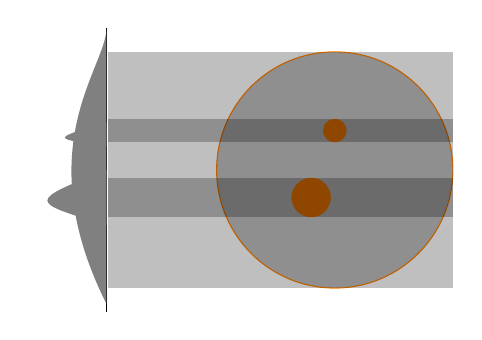
\begin{tikzpicture}[domain=3:3]  
		
		\fill[lightgray] (0.9,0.7) circle (1.5cm);
		
		\draw [rotate=90, yshift=2cm, - ](-1.1,0) -- (2.5,0); % s-Achse
		
		\fill[gray] [rotate=90, yshift=2cm] (-1,0) .. controls (1,1) and (2,0) .. (2.5,0);
		\fill[gray] [rotate=90, yshift=2cm] (0,0) .. controls (0.3,1)  .. (0.7,0);
		\fill[gray] [rotate=90, yshift=2cm] (1,0) .. controls (1.1,0.7)  .. (1.3,0);
		
		\draw[orange] (0.9,0.7) circle (1.5cm);
		\fill[orange] (0.9,  1.2) circle (.15cm);
		\fill[orange] (0.6, 0.35) circle (.25cm);
		
		\fill[nearly transparent] (-1.98,-0.8) rectangle (2.4,2.2);
		
		\fill[nearly transparent] (-1.98,0.1) rectangle (2.4,0.6);
		\fill[nearly transparent] (-1.98,1.05) rectangle (2.4,1.35);
		\begin{scope}[xshift=1cm]
		\end{scope}
		
		\end{tikzpicture} &	
		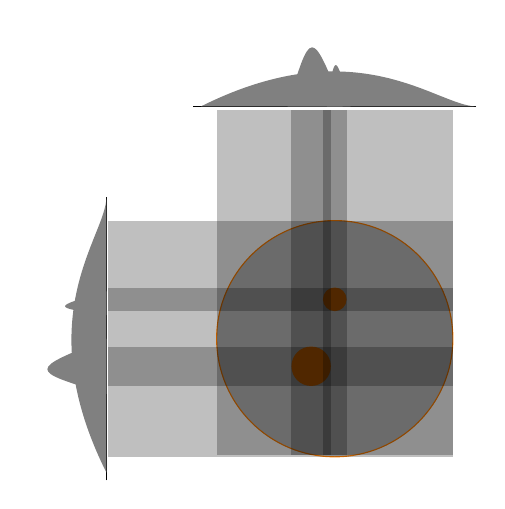
\begin{tikzpicture}[domain=3:3]  
		
		\fill[lightgray] (0.9,0.7) circle (1.5cm);
		
		\draw [rotate=90, yshift=2cm](-1.1,0) -- (2.5,0); % s-Achse
		
		\fill[gray] [rotate=90, yshift=2cm] (-1,0) .. controls (1,1) and (2,0) .. (2.5,0);
		\fill[gray] [rotate=90, yshift=2cm] (0,0) .. controls (0.3,1)  .. (0.7,0);
		\fill[gray] [rotate=90, yshift=2cm] (1,0) .. controls (1.1,0.7)  .. (1.3,0);
		
		\draw[orange] (0.9,0.7) circle (1.5cm);
		\fill[orange] (0.9,  1.2) circle (.15cm);
		\fill[orange] (0.6, 0.35) circle (.25cm);
		
		\fill[nearly transparent] (-1.98,-0.8) rectangle (2.4,2.2);
		
		\fill[nearly transparent] (-1.98,0.1) rectangle (2.4,0.6);
		\fill[nearly transparent] (-1.98,1.05) rectangle (2.4,1.35);
		\begin{scope}[xshift=1cm]
		\end{scope}
		
		\draw [rotate=0, yshift=3.65cm, xshift=0.2cm](-1.1,0) -- (2.5,0); % s-Achse
		
		\fill[gray] [rotate=0, yshift=3.65cm, xshift=0.2cm] (-1,0) .. controls (1,1) and (2,0) .. (2.5,0);
		\fill[gray] [rotate=0, yshift=3.65cm, xshift=0.3cm] (0,0) .. controls (0.3,1)  .. (0.7,0);
		\fill[gray] [rotate=0, yshift=3.65cm, xshift=-0.2cm] (1,0) .. controls (1.1,0.7)  .. (1.3,0);
		
		\fill[ nearly transparent] [rotate=90, xshift=1.1cm, yshift=-1.6cm] (-1.88,-0.8) rectangle (2.5,2.2);
		
		\fill[nearly transparent] [rotate=90, xshift=1.1cm, yshift=-0.95cm] (-1.88,0.1) rectangle (2.5,0.6);
		\fill[nearly transparent] [rotate=90, xshift=1.1cm, yshift=-2.1cm] (-1.88,1.05) rectangle (2.5,1.35);
		
		\end{tikzpicture}\\	
		(a) & (b) 
	\end{tabular}
	\caption{Das Prinzip der Bildrekonstruktion aus CT-Daten mit einer Rückprojektion~(a) und zwei Rückprojektionen~(b).} 
	\label{fig:1.2}
\end{figure}
%----------------------------------------------------------------------------------------
%	Ende der Grafik
%----------------------------------------------------------------------------------------

Ein Pionier der Tomographie, A. M. Cormack\footnote{\label{foot:1} Allan M. Cormack (1924-1998) südafrikanischer Physiker.}, veröffentlichte 1964 eine Arbeit über die mathematische Bestimmung der Dichten eines Objekts. Aus den Projektionsdaten konnte er die innere Dichteverteilung des Objekts bestimmen.

Der erste Prototyp eines CT-Scanners wurde vom G. N. Hounsfield\footnote{\label{foot:2} Godfrey N. Hounsfield (1919 - 2004) englischer Ingenieur.} im Jahr 1968 entwickelt. Seine Arbeit beruhte auf den Erkenntnissen von M. Cormack. Die Idee, der um das Objekt rotierenden Scanneinheit (Abb. \ref{fig:1.3}) findet man hier wieder. Vorerst konnten nur anatomische Präparate vermessen werden. Aber schon im Jahre 1972 entstehen erste klinische Untersuchungen mit einem Schädelscanner durch Hounsfield und Ambrose. 1973 werden Berichte über die Weichteildiagnostik des Gehirns mithilfe eines CT-Scanners veröffentlicht. Hinsichtlich der Nützlichkeit des CT-Verfahrens in der Medizin, wurden A. M. Cormack und G. N. Hounsfield im Jahre 1979 mit dem Nobelpreis für Medizin ausgezeichnet. 

In darauf folgenden Jahren entstand eine ganze Reihe von Generationen des CT-Scanners. Die Hauptunterschiede bestehen in der Komposition der Scanneinheit und dessen Technik, siehe auch \cite[Kap.\ 3]{Buzug04}. Heutzutage hat sich die dritte Genration am meisten durchgesetzt. Der prinzipielle Grundaufbau (Abb. \ref{fig:1.3}) dieses Scanners besteht darin, dass die Röntgenröhre und Detektor fest auf einem Ringkörper, einander gegenüber installiert sind. In der Mitte des Rings ist ein fest installierter Probetisch, sodass die Scanneinheit um diesen rotieren kann. Mittels dieser Konstruktion ist es möglich \textit{tomographische} Bilddaten aus allen Positionen um die Längsachse des Objekts aufzunehmen.
%----------------------------------------------------------------------------------------
%	Beginn der Grafik
%----------------------------------------------------------------------------------------
\begin{figure}[!h]
	
	\centering
	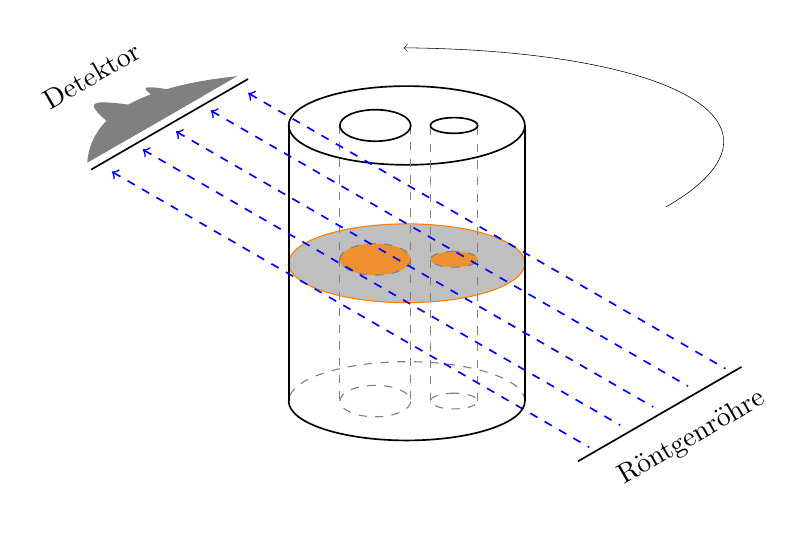
\begin{tikzpicture}
	%\draw[dashed,color=gray] [rotate=90, xshift=0cm, yshift=1.5cm] (-1,0) -- (4.4,0);% right line
	
	\draw[dashed,color=gray][rotate=90] (0,0) arc (-90:90:0.5 and 1.5);% top half of the bottom ellipse
	
	\draw[semithick][rotate=90] (4,1.5) arc (0:360:0.5 and 1.5);
	\draw[very thin, ->][rotate=95] (2.3,-2) arc (240:340:1.6 and 6);
	
	\fill[nearly transparent][rotate=90] (2.25,1.5) arc (0:360:0.5 and 1.5); % middle ellipse
	
	% inner lines
	\draw[dashed,color=gray] [rotate=90] (0,1.2) -- (3.5,1.2);% left line of inner small ellipse 
	\draw[dashed,color=gray] [rotate=90] (0,0.6) -- (3.5,0.6);% right line of the inner small ellipse
	
	\draw[dashed,color=gray] [rotate=90] (3.5, 2.35) -- (0, 2.35);% right line of the inner big ellipse
	\draw[dashed,color=gray] [rotate=90] (3.5, 1.45) -- (0, 1.45);% left line of the inner big ellipse
	
	% inner top ellipses
	\draw[semithick] [rotate=90] (3.5, .9) ellipse (0.1 and .3); % top small inner ellipse
	\draw[semithick] [rotate=90] (3.5, 1.9) ellipse (0.2 and .45); % top big inner ellipse
	
	% inner middle ellipses
	\fill[nearly opaque,color=orange] [rotate=90] (1.8, .9) ellipse (0.1 and .3);% middle small inner ellipse
	\fill[nearly opaque,color=orange] [rotate=90] (1.8, 1.9) ellipse (0.2 and .45); % middel big inner ellipse
	\draw[dashed,color=gray] [rotate=90] (1.8, .9) ellipse (0.1 and .3);% middle small inner ellipse
	\draw[dashed,color=gray] [rotate=90] (1.8, 1.9) ellipse (0.2 and .45); % middel big inner ellipse
	
	
	% inner bottom ellipses
	\draw[dashed,color=gray] [rotate=90] (0, .9) ellipse (0.1 and .3); % bottom small inner ellipse
	\draw[dashed,color=gray] [rotate=90] (0, 1.9) ellipse (0.2 and .45); % bottom big innerellipse
	
	\draw[color=orange][rotate=90] (2.25,1.5) arc (0:360:0.5 and 1.5); % middle ellipse
	
	%sids lines
	\draw[semithick] [rotate=90] (0,0) -- (3.5,0);% right line
	\draw[semithick] [rotate=90] (0,3) -- (3.5,3);% left line
	
	% Röntgenröhre
	\draw [semithick] [rotate=30, xshift=0.cm, yshift=-1.0cm](0.2,0) -- (2.6,0); % Röntgenröhre
	\draw  (1.5,-1.4) node [rotate=30, xshift=1.cm, yshift=0.5cm] { Röntgenröhre};
	
	\draw [semithick] [rotate=30, xshift=-3.5cm, yshift=5.3cm](0.2,0) -- (2.5,0); % Detektorachse
	\draw  (1.5,-1.4) node [rotate=30, xshift=-3.3cm, yshift=8.3cm] {Detektor};
	
	\draw [dashed, semithick, <-, blue] [rotate=150, , xshift=1.cm, yshift=0.1cm](5,0) -- (-2,0);
	\draw [dashed, semithick, <-, blue] [rotate=150, , xshift=0.8cm, yshift=-0.34cm](5,0) -- (-2,0);
	\draw [dashed, semithick, <-, blue] [rotate=150, , xshift=0.55cm, yshift=-0.75cm](5,0) -- (-2,0);
	\draw [dashed, semithick, <-, blue] [rotate=150, , xshift=0.3cm, yshift=-1.2cm](5,0) -- (-2,0);
	\draw [dashed, semithick, <-, blue] [rotate=150, , xshift=3.cm, yshift=-1.63cm](2,0) -- (-5,0);
	
	\fill[gray] [rotate=30, yshift=5.4cm, xshift=-3cm] (-0.3,0) .. controls (0.1,0.6) and (1,0.4) .. (1.9,0);
	\fill[gray] [rotate=30, yshift=5.4cm, xshift=-3cm] (0.3,0) .. controls (0,0.8)  .. (1,0);
	\fill[gray] [rotate=30, yshift=5.4cm, xshift=-3cm] (1,0) .. controls (0.7,0.6)  .. (1.4,0);
	
	\draw[semithick] [rotate=90] (0,0) arc (270:90:0.5 and 1.5);% bottom half of the bottom ellipse
	
	\end{tikzpicture}
	\caption{Prinzipieller Aufbau eines CT-Scanners der dritten Generation.}
	\label{fig:1.3}
\end{figure}
%----------------------------------------------------------------------------------------
%	Ende der Grafik
%----------------------------------------------------------------------------------------
Die oben beschriebene Rückprojektion aller tomographischen Daten (Projektionen) erzeugt ein Schnittbild. Erzeugt man mehrere Schnittbilder entlang der Längsachse des Objekts, so kann man diese der Reihe nach aufstellen und mithilfe programmiertechnischer Werkzeuge ein dreidimensionales Bild dieses Objekts gewinnen (Abb. \ref{fig:1.4}) .
%----------------------------------------------------------------------------------------
%	Beginn der Grafik
%----------------------------------------------------------------------------------------
\begin{figure}[h]
	\centering
	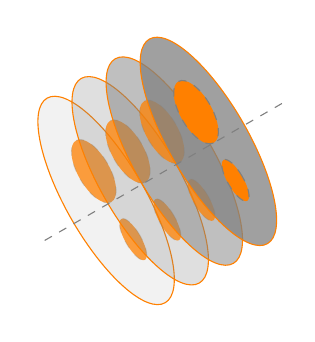
\begin{tikzpicture}
	
	\fill[very nearly transparent, color=gray][rotate=30] (2.25,1.5) arc (0:360:0.5 and 1.5); % middle ellipse
	
	% inner middle ellipses
	\fill[nearly opaque,color=orange] [rotate=30] (1.8, .9) ellipse (0.1 and .3);% middle small inner ellipse
	\fill[nearly opaque,color=orange] [rotate=30] (1.8, 1.9) ellipse (0.2 and .45); % middel big inner ellipse
	\draw[nearly transparent, dashed,color=gray] [rotate=30] (1.8, .9) ellipse (0.1 and .3);% middle small inner ellipse
	\draw[nearly transparent, dashed,color=gray] [rotate=30] (1.8, 1.9) ellipse (0.2 and .45); % middel big inner ellipse
	
	\draw[color=orange][rotate=30] (2.25,1.5) arc (0:360:0.5 and 1.5); % middle ellipse
	
	%--------- second slice
	
	\fill[nearly transparent, color=gray][rotate=30, xshift=0.5cm] (2.25,1.5) arc (0:360:0.5 and 1.5); % middle ellipse
	
	% inner middle ellipses
	\fill[nearly opaque,color=orange] [rotate=30, xshift=0.5cm] (1.8, .9) ellipse (0.1 and .3);% middle small inner ellipse
	\fill[nearly opaque,color=orange] [rotate=30, xshift=0.5cm] (1.8, 1.9) ellipse (0.2 and .45); % middel big inner ellipse
	\draw[nearly transparent, dashed,color=gray] [rotate=30, xshift=0.5cm] (1.8, .9) ellipse (0.1 and .3);% middle small inner ellipse
	\draw[nearly transparent, dashed,color=gray] [rotate=30, xshift=0.5cm] (1.8, 1.9) ellipse (0.2 and .45); % middel big inner ellipse
	
	\draw[color=orange][rotate=30, xshift=0.5cm] (2.25,1.5) arc (0:360:0.5 and 1.5); % middle ellipse
	
	%--------- third slice
	
	\fill[semitransparent, color=gray][rotate=30, xshift=1cm] (2.25,1.5) arc (0:360:0.5 and 1.5); % middle ellipse
	
	% inner middle ellipses
	\fill[nearly opaque, color=orange] [rotate=30, xshift=1cm] (1.8, .9) ellipse (0.1 and .3);% middle small inner ellipse
	\fill[nearly opaque, color=orange] [rotate=30, xshift=1cm] (1.8, 1.9) ellipse (0.2 and .45); % middel big inner ellipse
	\draw[nearly transparent, dashed,color=gray] [rotate=30, xshift=1cm] (1.8, .9) ellipse (0.1 and .3);% middle small inner ellipse
	\draw[nearly transparent, dashed,color=gray] [rotate=30, xshift=1cm] (1.8, 1.9) ellipse (0.2 and .45); % middel big inner ellipse
	
	\draw[color=orange][rotate=30, xshift=1cm] (2.25,1.5) arc (0:360:0.5 and 1.5); % middle ellipse
	
	%--------- fourd slice	
	
	\fill[nearly opaque, color=gray] [rotate=30, xshift=1.5cm] (2.25,1.5) arc (0:360:0.5 and 1.5); % middle ellipse
	
	% inner middle ellipses
	\fill[color=orange] [rotate=30, xshift=1.5cm] (1.8, .9) ellipse (0.1 and .3);% middle small inner ellipse
	\fill[color=orange] [rotate=30, xshift=1.5cm] (1.8, 1.9) ellipse (0.2 and .45); % middel big inner ellipse
	\draw[dashed,color=gray] [rotate=30, xshift=1.5cm] (1.8, .9) ellipse (0.1 and .3);% middle small inner ellipse
	\draw[dashed,color=gray] [rotate=30, xshift=1.5cm] (1.8, 1.9) ellipse (0.2 and .45); % middel big inner ellipse
	
	\draw[color=orange] [rotate=30, xshift=1.5cm] (2.25,1.5) arc (0:360:0.5 and 1.5); % middle ellipse
	
	\draw[dashed,color=gray] [rotate=30, xshift=0.8cm] (3.5, 1.45) -- (0, 1.45); % axisis
	
	\end{tikzpicture}
	\caption{Das Schichtmodell eines Objekts als Grundlage zur dreidimensionalen Rekonstruktion.}
	\label{fig:1.4}
\end{figure} 
%----------------------------------------------------------------------------------------
%	Ende der Grafik
%----------------------------------------------------------------------------------------

Im Folgenden gehen wir mehr auf die mathematisch-physikalischen Gegebenheiten der oben beschriebenen Situation ein. 

\section*{Die Radon Transformation}
\label{cha:1.2}

Das Verständnis des mathematischen Problems der Bildrekonstruktion in der Computertomographie verlangt zunächst das Verständnis der Entstehung der tomographischen Bilddaten. Die Entstehung solcher Daten kann mithilfe eines mathematischen Modells nachvollzogen werden. Bekanntlich baut man das mathematische Modell auf physikalischen Annahmen auf. Die Abbildung \ref{fig:1.5} soll in diesem Fall als physikalisches Ausgangsmodell dienen. Wir nehmen an, dass der graue Kreis eine homogene Dichteverteilung besitzt. Unter weiteren Annahme sollen die Röntgenstrahlen sich geradlinig ohne Streuung in Richtung des Detektors ausbreiten.

Sei nun $f(x,y)$ die gesuchte Dichtefunktion, die auf einem Einheitskreis $\Omega = \{ (x,y) \in \R^2 \ | \ x^2 + y^2 \leq 1 \}$ definiert ist. Dass $f$ auf einem Kreis liegen soll, folgern wir aus der physikalischen Situation. Das Objekt wird aus einem bestimmten Radius um den Mittelpunkt der Scanneinheit gescannt, daher möchten wir, dass ein Objekt in die CT-Scanneinheit passt, gegebenenfalls muss die Scanneinheit skaliert werden.

Die blau gestrichelte Linie in Abbildung \ref{fig:1.5} stelle einen Röntgenstrahl dar. Wir möchten das Verhalten der Intensität entlang der Strahllinie an den Punkten $L_0$ und $L_0 + \Delta L$ beobachten. Wie schon erwähnt wurde, nimmt die Intensität $I$ der Röntgenstrahlen mit der Eindringtiefe in das Objekt ab. Das Verhalten ist in der Physik unter dem Namen \textit{Lambert-Beer’sches Gesetz} bekannt und besagt:
\begin{center}
	\textit{Die Intensitätsabnahme der Strahlung ist proportional zur Intensität. Der Proportionalitätsfaktor hängt von der Art der durchdrungenen Materie ab.}
\end{center}
\begin{equation}
	I(L_0 + \Delta L) - I(L_0) = - \alpha I(L_0).
	\label{equa:1.100}
\end{equation}
Der Proportionalitätsfaktor $\alpha$ ist durch das Produkt der Dichteverteilung entlang des Strahls, also $f(L)$ und seiner zurückgelegten Strecke $\parallel \Delta L\parallel$ gegeben. Hier wird angenommen, dass $f(L)$ die Eigenschaften des Materials in sich trägt. Insgesamt ergibt sich
\begin{equation}
	I(L_0 + \Delta L) - I(L_0) = -f(L) \parallel \Delta L \parallel I(L_0).
	\label{equa:1.2}
\end{equation}
Nimmt man an, dass die Gleichung (\ref{equa:1.2}) asymptotisch im Sinne $\parallel \Delta L \parallel \rightarrow 0$ verstanden werden kann, so kann die linke Seite von (\ref{equa:1.2}) als Ableitung von $I$ nach $L$ interpretiert werden und man schreibt:
\begin{equation}
	\lim_{\Delta L\rightarrow 0}\frac{I(L_0 + \Delta L) - I(L_0)}{\parallel \Delta L \parallel} = \frac{\partial I}{\partial L} = -f(L)I(L_0).
	\label{equa:1.3}
\end{equation}
Mit \ref{equa:1.3} liegt eine lineare Differentialgleichung (DGL) erster Ordnung vor. Diese DGL kann mithilfe einfacher analytischer Werkzeuge, wie Variablenseparation gelöst werden. 
%----------------------------------------------------------------------------------------
%	Beginn der Grafik
%----------------------------------------------------------------------------------------
\begin{figure}[!h]
	\centering
	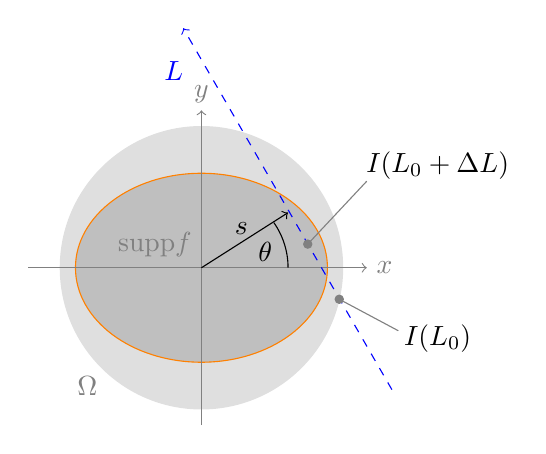
\begin{tikzpicture}

	\fill[nearly transparent, color=gray] (0.9,0) circle (1.8cm);
	
	\fill[lightgray] (0.9,0) ellipse (1.6cm and 1.2cm);	
	
	\draw[orange] (0.9,0) ellipse (1.6cm and 1.2cm);
	
	\draw [gray] [->](-1.3,0) -- (3,0); % x-Achse
	\draw [gray] (3, 0) node [right] {$x$};
	
	\draw [gray] [->](0.9,-2) -- (0.9,2); % y-Achse
	\draw [gray] (0.9, 2.2) node {$y$};
	
	\draw[gray](0.9, 0.3) node [left] {$\mbox{supp}f$};
	
	\draw[->] (0.9,0) -- (2, 0.7);
	\draw(1.2, 0.5)  node [right] {$s$};
	
	\draw [rotate=30, xshift=2.1cm, dashed, ->] [blue] (0,-3) -- (0,2.3); % strahl
	\draw [blue] (0.55, 2.5)  node {$L$};
	
	\draw(2,0) arc [start angle=0, end angle=35, radius=1cm];
	\draw(1.5, 0.2) node [right] {$\theta$};
	
	\draw [gray] (-0.8, -1.5) node [right] {$\Omega$};
	
	\draw(3.9, 1.3) node {$I(L_0 + \Delta L)$};
	\fill[gray](2.25, 0.3) circle [radius=0.06];
	\draw[-,thin,gray](2.25, 0.3) -- (3, 1.1);
	
	\draw(3.9, -0.9) node {$I(L_0)$};
	\fill[gray](2.65, -0.4) circle [radius=0.06];
	\draw[-,thin,gray](2.65, -0.4) -- (3.4, -0.8);
	
	\end{tikzpicture}	
	\caption{Intensitätsänderung der Röntgenstrahlung beim Passieren eines homogenen Objekts.}
	\label{fig:1.5}
\end{figure}
%----------------------------------------------------------------------------------------
%	Ende der Grafik
%----------------------------------------------------------------------------------------
Nach der Separation der Variablen in (\ref{equa:1.3}) und anschließender Integration bekommt man nun folgenden Ausdruck
\begin{equation}
	\ln(\frac{I_1}{I_0}) = -\int_{L_0}^{L_1} f(L) \mbox{d} L.
	\label{equa:1.4}
\end{equation}
Durch das Exponentieren von (\ref{equa:1.4}) gelangt man zu dem \textit{Lambert-Beer’schen Gesetz} $I(L_1) = I_0 e^{-\int_{L_0}^{L_1} f(L) \mbox{d} L}$. Jedoch für die Zwecke der Computertomographie interessiert man sich für etwas von (\ref{equa:1.4}) abgewandelte Darstellung
\begin{equation}
	\ln(\frac{I_0}{I_1}) = \int_{L_0}^{L_1} f(L) \mbox{d} L.
	\label{equa:1.5}
\end{equation} 
Die rechte Seite in (\ref{equa:1.5}) liefert einen Summenwert von $f$ entlang der Geraden $L$ (Abb. \ref{fig:1.6}), die wie folgt parametrisiert werden kann:
\begin{equation}
	\begin{matrix}
		L(s, \theta, t) & = & s\begin{pmatrix} \cos(\theta) \\ \sin(\theta) \end{pmatrix} & + & t\begin{pmatrix} -\sin(\theta) \\ \cos(\theta)  \end{pmatrix} \\ \\
		& = & s\omega(\theta) & + & t\omega^{\perp}(\theta)
	\end{matrix} \ , \ \ s, t \in \R; \ \theta \in [0,\pi].
	\label{equa:1.6}
\end{equation}
Betrachtet man alle Geraden, die den Einheitskreis schneiden, dann ergibt sich folgende Menge
\begin{equation}
	G = \{ L(s, \theta, t) \ | \ |s| \leq 1, \  \theta \in [0,\pi] \ t \in [-\gamma(s), \gamma(s)] \}.
	\label{equa:1.7}
\end{equation}
Wobei $\gamma(s)$ den Parameter $t$ für (\ref{equa:1.6}) festlegt und folgendermaßen definiert werden kann
\begin{equation}
	\gamma(s) = \left\{ \begin{matrix}
	\sqrt{1 - s^2} & : & |s| \leq 1 \\ 
	0 & : & \mbox{sonst}
	\end{matrix}.
	\right.
	\label{equa:1.8}
\end{equation}
Die Gleichung (\ref{equa:1.8}) liefert nun die Integrationsgrenzen für (\ref{equa:1.5}). Da die Werte von $\pm\gamma(s)$ genau die Schnittpunkte von $L$ mit $\Omega$ liefern und  $\mbox{supp} f$\footnote{\label{foot:3} Mit $\mbox{supp} f$ (Support) ist der Träger einer Funktion $f$ gemeint. Def.: $\mbox{supp} f := \overline{ \{ x \in \Omega | f(x) \neq 0 \} } $} $\subseteq \Omega$, heißt es insgesamt, dass nur die Werte von $L \subset \mbox{supp} f$ bei der Integration von (\ref{equa:1.5}) berücksichtigt werden.

Kehren wir zur Gleichung (\ref{equa:1.5}) zurück und betrachten die Abbildung \ref{fig:1.6}, werden wir feststellen, dass die Funktion $f$ über den Parameter $t$ integriert werden muss. Hierzu bedarf es einer Variablentransformation:
\begin{equation}
	\begin{matrix}
		|(J(L))| = \left|\begin{pmatrix} \cos(\theta) & \sin(\theta)\\ -\sin(\theta) & \cos(\theta) \end{pmatrix}\right| = 1 \\ \\
		\mbox{und} \\ \\
		\mbox{d}L = \mbox{det}(J(L)) \mbox{d}t .
	\end{matrix}
	\label{equa:1.9}
\end{equation}
%----------------------------------------------------------------------------------------
%	Beginn der Grafik
%----------------------------------------------------------------------------------------
\begin{figure}[!h]
	\centering
	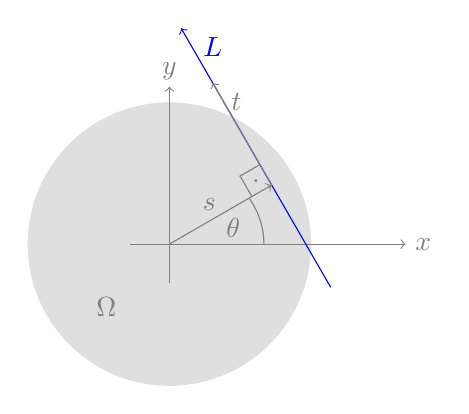
\begin{tikzpicture}
	
	\fill[nearly transparent, color=gray] (0,0) circle (1.8cm);
	
	\draw [gray] [->](-0.5,0) -- (3,0); % x-Achse
	\draw [gray] (3, 0) node [right] {$x$};
	
	\draw [gray] [->](0,-0.5) -- (0,2); % y-Achse
	\draw [gray] (0, 2.2) node {$y$};
	
	\draw [rotate=30, xshift=1.5cm, ->] [blue] (0,-1.5) -- (0,2.3); % strahl	
	\draw [blue] (0.55, 2.5)  node {$L$};%{$\omega^{\perp}$};
	
	\draw [rotate=30, xshift=1.5cm, ->] [gray ] (0,0) -- (0,1.5);
	\draw [gray] (0.85,1.8) node {$t$}; 
	
	\draw [xshift=1.05cm, yshift=0.6cm, rotate=120, - ] [gray] (0,0) -- (0.3,0);
	\draw [xshift=0.89cm, yshift=0.86cm, rotate=30, - ] [gray] (0,0) -- (0.3,0);
	\draw [gray] (1.1, 0.8)  node {$.$};
	
	\draw [rotate=30] [gray] [->] (0,0) -- (1.5, 0);
	\draw [gray] (0.3, 0.5)  node [right] {$s$};
	
	\draw [gray] (1.2,0) arc [start angle=0, end angle=35, radius=1cm];
	\draw [gray] (0.6, 0.2) node [right] {$\theta$};
	
	\draw [gray] (-0.8, -0.8) node {$\Omega$};
	
	\end{tikzpicture}
	\caption{Parametrisierung des Strahls $L$ auf dem Gebiet $\Omega$. }
	\label{fig:1.6}
\end{figure}
%----------------------------------------------------------------------------------------
%	Ende der Grafik
%----------------------------------------------------------------------------------------

Mit den obigen Abmachungen haben wir nun alles Nötige in der Hand, um die Radon\footnote{\label{foot:4} Johann Karl August Radon (1887-1956) österreichischer Mathematiker.} Transformation angeben zu können. 
\begin{Definition}
	Sei nun $f:\Omega \subseteq \R^2 \rightarrow \R$ eine integrierbare Funktion, dann ist ihre Radon Transformation durch
	\begin{equation}
		\mathcal{R}f(s,\theta) := \int\limits_{-\gamma(s)}^{\gamma(s)} f(s\omega(\theta) + t\omega^{\perp}(\theta)) \mbox{d}t
		\label{equa:1.10}
	\end{equation}
	definiert. Hier ist $\Omega = \{ (x,y) \in \R^2 \ | \ x^2 + y^2 \leq 1 \}$.
	\label{def.1}
\end{Definition}

\begin{Bemerkung}
	$\mathcal{R}$ wird als Integraloperator oder einfach als Operator bezeichnet.
	\label{bem:1} 
\end{Bemerkung}

Die Gleichung (\ref{equa:1.10}) trägt das Wesen der Computertomographie in sich und gehört in den Bereich der Integraltransformationen. In der Tat ist man aber an der Inversion von $\mathcal{R}$ interessiert. Das wird klarer, wenn man (\ref{equa:1.10}) etwas anders auffasst:
\begin{equation}
	p(s,\theta) = \mathcal{R}f(s,\theta).
	\label{equa:1.11}
\end{equation}
Somit stellt $p(s,\theta)$ in (\ref{equa:1.11}) genau die Projektion einer unbekannten Dichteverteilung entlang eines Röntgenstrahls $L(s,\theta)$ dar. Da die Projektionen als Messwerte beim CT-Verfahren entstehen, möchte man $f$ folgendermaßen wiedergewinnen 
\begin{equation}
	f(x) = \mathcal{R}^{-1}p(x).
	\label{equa:1.12}
\end{equation}
Jedoch offenbaren sich einige mathematische Hürden bei der Inversion von (\ref{equa:1.10}), was die Rekonstruktion von $f$ aus den Projektionsdaten schwierig macht. Um die dahinterstehende Problematik besser verstehen zu können, untersuchen wir zunächst die Eigenschaften von (\ref{equa:1.10}).

\subsection*{Kleiner Einschub über $L^2$-Raum}
\label{cha:1.2.1}

Um den Operator $\mathcal{R}$ untersuchen zu können, sollte man wissen auf welchen Räumen er operiert. Dieses Wissen erlaubt uns Aussagen über die Stetigkeit, Kompaktheit und auch über die Singulärwertzerlegung (SWZ) von $\mathcal{R}$ zu treffen. Besonders wichtig ist die SWZ, denn anhand dieser ergibt sich eine Möglichkeit den Operator $\mathcal{R}$ zu invertieren. Zudem wollen wir im nächsten Kapitel die Schlechtgestelltheit des computertomographischen Problems diskutieren, welche die Eigenschaften der SWZ benutzt.

In Bezug auf das hier vorgestellte Rekonstruktionsproblem der Computertomographie betrachten wir Funktionen auf dem Gebiet $\Omega \subset \R^2$. Wir setzen voraus, dass die Funktionen auf $\Omega$ integrierbar sind. Wie dieser Sachverhalt zu verstehen ist, wollen wir kurz und grob andeuten.

Zunächst klären wir den Begriff der Integrierbarkeit einer Funktion im Sinne von Lebesgue\footnote{Henri Léon Lebesgue (1875-1941) französischer Mathematiker.}. Das Lebesgue-Integral wird für Funktionen auf einem geeigneten Maßraum definiert. Ein Maßraum ist durch ein Tripel $( \Omega, \mathcal{A}, \lambda)$ gegeben.

Eine sogenannte $\sigma$-\textit{Algebra} $\mathcal{A} \subset \mathcal{P}(\Omega)$ auf $\Omega$ ist ein Mengensystem bestehend aus Teilmengen von $\Omega$. $\mathcal{A}$ besitzt folgende Eigenschaften: (\lowroman{1}). Jede endliche oder abzählbar unendliche Vereinigung oder jeder Durchschnitt der Elemente aus $\mathcal{A}$ liegen wieder in $\mathcal{A}$, sowie $\Omega$ und $\emptyset$. (\lowroman{2}). Die Komplemente der Elemente aus $\mathcal{A}$, also $\forall A \in \mathcal{A} : \Omega \setminus A = A^\mathrm{C} \in \mathcal{A}$ , liegen auch in $\mathcal{A}$.

Nun suchen wir eine Funktion, die allen Elementen $A$ aus $\mathcal{A}$ eine positive Zahl zuordnet, also $\lambda(A) \in [0, \infty]$. Somit beschreibt $\lambda$ das Maß einer Menge in $\mathcal{A}$. Im Falle $\Omega \subset \R^2$ ordnet $\lambda$ den Flächeninhalt einer Teilmenge von $\Omega$ zu. Des Weiteren hat $\lambda$ folgende Eigenschaften: (\lowroman{1}): $\lambda(\emptyset) = 0$ und (\lowroman{2}): die $\sigma$-\textit{Additivität}, das heißt für paarweise disjunkte Mengen $(A_n)_{n \in \N}$ aus $\mathcal{A}$ gilt
 
\[ \lambda \left(  \bigcup\limits_{n=1}^{\infty} A_n \right) = \sum\limits_{n = 1}^{\infty} \lambda(A_n).\]  

Nun gilt per Definition \textit{messbarer Abbildungen} zwischen zwei Maßräumen, dass die Urbilder messbarer Mengen messbar sind. Das heißt $f:(X_1, \mathcal{A}_1) \rightarrow (X_2, \mathcal{A}_2)$ ist messbar, wenn für alle $A_{2_j} \in \mathcal{A}_2$ gilt $f^{-1}(A_{2_j}) \in \mathcal{A}_1$. 

Um den Begriff der Integrierbarkeit im Sinne von Lebesgue einführen zu können, fehlt uns noch der Begriff der Borel\footnote{Émile Borel (1871-1956)  französischer Mathematiker.}-$\sigma$-Algebra. Dazu benutzen wir für uns relevante mengen $\R$ und $\R^2$. Das ist insofern klar, weil die gesuchten Dichtefunktionen in einem Punkt $x \in \Omega \subset \R^2$ einen skalaren Wert $f(x) \in \R$ liefern. Noch legen wir fest, dass die Werte der Funktionen auf $\Omega$ immer positiv sind, also $f(x) \in \R^+$, denn es gibt keine negativen Dichten. Betrachten wir den topologischen Raum $(\R,\mathcal{T})$, hier stellt $\mathcal{T}$ \footnote{
Sei $X$ eine Menge, dann ist $\mathcal{T} \subset 2^{X}$ eine Topologie auf X, falls folgendes gilt:
\begin{itemize}
	\item[(i)] $\emptyset , X \subset \mathcal{T}$. 
	\item[(ii)] $ A,B \subset X \in \mathcal{T} \Rightarrow A \cap B \in \mathcal{T}$.
	\item[(iii)] $\{ A_{_i}\}_{_{i \in I}} \in \mathcal{T} \Rightarrow \bigcup\limits_{i \in I} A_{_i} \in \mathcal{T}$ 
\end{itemize}
So nennt man das Paar $(X, \mathcal{T})$ ein topologischer Raum. Alle Elemente von $\mathcal{T}$ sind offene Mengen.}
ein System von offenen Mengen von $\R$ dar, dann heißt $\mathcal{B}(\R)$ die von $\mathcal{T}$ erzeugte $\sigma$-Algebra auf $\R$, die Borel-$\sigma$-Algebra. $\mathcal{B}(\R)$ ist die kleinste Algebra, die $\mathcal{T}$ enthält. Das bringt uns ein Vorteil bezüglich der Messbarkeit, denn somit erhalten wir die größtmögliche Menge messbarer Mengen von $\R$. Für $\R^2$ gilt das Obere auch.

Im letzten Schritt definieren wir die sogenannten positiven Treppenfunktionen $h^+:(\Omega, \mathcal{B}(\Omega)) \rightarrow (\R, \mathcal{B}(\R))$, die endlich viele Werte $c_j \in \R_{0}^{+}, \ j \in [1,n], \ n \in \N$ auf $\Omega$ annehmen. Auf diese Weise ist es möglich das Integral über $h^+$ folgendermaßen anzugeben:

\[ \mathcal{I}(h^+) = \sum\limits_{j = 1}^{n} c_j \lambda({A_j}), \ \ \mbox{für } A_j \in \mathcal{B}(\Omega).\]

Jetzt können wir das Lebesgue-Integral einer messbaren Funktion $f: \Omega \rightarrow \R^+$ definieren, indem wir die Funktion $f$ `von unten' mit Treppenfunktionen approximieren:
\begin{Definition}
	Sei  $f: \Omega \rightarrow \R^+$ messbar, dann ist sie integrierbar im Sinne von Lebesgue, wenn gilt
	\[ \int\limits_{\Omega} f(x) = \sup\{ \mathcal{I}(h^+) | \forall x \in \Omega : h^+(x) \leq f(x) \} < \infty.\]
	\label{def.2}
\end{Definition}
\begin{Bemerkung}
	Im Falle einer Lebesgue-Integrierbarkeit spricht man meistens davon, dass eine Funktion Integrierbar ist. Streng genommen müsste man das Lebesgue-Integral für beliebige Funktionen $f:\Omega \rightarrow \R$ mit einer geeigneten Fortsetzung einführen, um dem Begriff der Integrierbarkeit gerecht zu werden. Aber die Definition \ref{def.2} reicht uns, um das Prinzip der Integration verstanden zu haben. 
	\label{bem:2}
\end{Bemerkung}
Nun sind wir im Stande den \textit{Raum der quadratintegrierbarer Funktionen} folgendermaßen zu definieren:
\begin{equation}
	\mathcal{L}^{2}(\Omega, \mathcal{A}, \lambda) = \{ f : \Omega \rightarrow \R \ | \ f \mbox{ ist integrierbar und } \int \limits_{\Omega} |f(x)|^2 \mbox{d}x \leq \infty \}.
	\label{equa:1.13}
\end{equation}
Versehen wir den Raum $\mathcal{L}^{2}(\Omega, \mathcal{A}, \lambda)$ mit einer Norm
\begin{equation}
	\Vert f \Vert_2 := \ < f, f >^{\frac{1}{2}} \ = \left( \int |f(x)|^2 \mbox{d}x \right)^{\frac{1}{2}}, \ \ x \in \Omega,
	\label{equa:1.14}
\end{equation}
so erhalten wir den Raum $L^2(\Omega, \mathcal{A}, \lambda)$ (einfach $L^2(\Omega)$), also den \textit{Hilbertraum der quadratintegrierbaren Funktionen}. 

Im Allgemeinen ist $L^2(\Omega)$ ein unendlichdimensionaler Vektorraum über dem Körper der komplexen Zahlen, der bezüglich der durch das Skalarprodukt induzierten Norm vollständig ist.

Kehren wir zurück, zu den gesuchten Funktionen auf einer Kreisscheibe $\Omega$, dann sei das Urbild des Operators $\mathcal{R}$ genau die Menge $L^2(\Omega)$. Das Bild von $\mathcal{R}$ liegt jedoch auf einem halben Zylinder $Z := [0, \pi] \times [-1,1]$. Der Grund hierfür ist ein technischer, denn bei Projektionen über den ganzen Durchmesser einer Kreisfläche auf einem Intervall von $0$ bis $2\pi$, entstehen redundante Daten, also reichen die Projektionen von $0$ bis $\pi$. 

Des Weiteren  wissen wir an dieser Stelle noch nicht wohin $\mathcal{R}$ den Raum $L^2(\Omega)$ abbildet. Aber wie oben schon erwähnt wurde, wollen wir später die SWZ von $\mathcal{R}$ angeben, dafür muss ein \textit{adjungierter} Operator $\mathcal{R^*}$ zu $\mathcal{R}$ existieren\footnote{\label{foot:5} Der Grund weshalb $\mathcal{R^*}$ existieren muss ist folgender: Es kann nicht vorausgesetzt werden, dass $\mathcal{R}$ selbstadjungiert ist, wonach der \textit{Spektralsatz für selbstadjungierte Operatoren} für $\mathcal{R}$ nicht gelten würde. Aber für $\mathcal{R}\mathcal{R^*}$ funktioniert der Satz schon, da $\mathcal{R}\mathcal{R^*} = (\mathcal{R}\mathcal{R^*})^* = \mathcal{R^*}\mathcal{R}$ gelte.}. Um das zu bewerkstelligen, muss man fordern, dass der Bildraum sowie der Kern von $\mathcal{R}$ Orthogonalbasen besitzen sollen, was auch einen Skalarprodukt impliziert. Hieraus kann eine Vermutung aufgestellt werden, dass $\mathcal{R}$ $L^2(\Omega)$ nach $L^2(Z)$ abbilden soll, weil eben $L^2$ Räume der Forderung gerecht sind. Somit erhalten wir insgesamt
\begin{equation}
	\mathcal{R} : L^2(\Omega) \rightarrow L^2(Z).
	\label{equa:1.15}
\end{equation}
Mit (\ref{equa:1.15}) kann man die Eigenschaften des Operators $\mathcal{R}$ gut untersuchen.

\subsection*{Eigenschaften der Radon Transformation}
\label{cha:1.2.2}

In diesem Kapitel sollen einige Eigenschaften des Operators $\mathcal{R}$ erarbeitet werden. Anhand der Eigenschaften von $\mathcal{R}$ kann die Problematik der Gleichung (\ref{equa:1.12}) besser verstanden werden. Zunächst zeigen wir die Linearität von $\mathcal{R}$. 
\subsubsection{Linearität von $\mathcal{R}$}
$\mathcal{R}$ ist linear, denn für $f, g \in L^2(\Omega)$ beliebig,  ergibt sich 
\begin{equation}
	\begin{split}
		\mathcal{R}( \alpha f + \beta g) & \stackrel{\mbox{\scriptsize Def.}\ref{def.1}}{=}  \int\limits_{-\gamma(s)}^{\gamma(s)} \left( \alpha f + \beta g\right ) \mbox{d}t\\
		& \stackrel{\mbox{\scriptsize Lin.}}{=} \alpha \int\limits_{-\gamma(s)}^{\gamma(s)} f\mbox{d}t  +  \beta \int\limits_{-\gamma(s)}^{\gamma(s)} g \mbox{d}t\\
		& = \alpha \mathcal{R} f +  \beta \mathcal{R} g .
	\end{split}
	\label{equa:1.16}
\end{equation}
Der Übersichtlichkeit halber wurden in (\ref{equa:1.16}) die Argumente weggelassen, also für alle $f \in \Omega$ gilt $f = f(s\omega(\theta) + t\omega^{\perp}(\theta))$.

\subsubsection{Stetigkeit von $\mathcal{R}$}

Mit dem obigen Ergebnis kann man die Theorie der linearen Operatoren in normierten Räumen auf $\mathcal{R}$ anwenden. Nun wollen wir die Stetigkeit von $\mathcal{R}$ überprüfen.
\begin{lemma}
	Der Operator $R : L^2(\Omega) \rightarrow L^2(Z)$ ist stetig.
	\label{lemma:1}
\end{lemma}
\begin{proof}
	Das Ziel ist zu zeigen, dass das Bild von $\mathcal{R}$ beschränkt ist. Demnach ist jeder linearer beschränkter Operator stetig (s.a. \cite[S.82]{Burg91}). Wir führen den Beweis in zwei Schritten durch. Zuerst geben wir eine Abschätzung für $|\mathcal{R} f(s,\theta)|^2$ und dann für $\Vert \mathcal{R} \Vert_2$.
	\begin{enumerate}
		\item[\lowroman{1}.] Sei nun $f \in L^2(\Omega)$ beliebig, dann gilt mit Benutzung der Cauchy-Schwarzschen Ungleichung für Integrale
		\begin{equation}
			\begin{split}
				|\mathcal{R} f(s,\theta)|^2 & = \left| \ \int\limits_{-\gamma(s)}^{\gamma(s)} f(s\omega(\theta) + t\omega^{\perp}(\theta)) \mbox{d}t \ \right|^2 \\
				& \leq \int\limits_{-\gamma(s)}^{\gamma(s)} 1 \mbox{d}t \int\limits_{-\gamma(s)}^{\gamma(s)} |f(s\omega(\theta) + t\omega^{\perp}(\theta))|^2 \mbox{d}t\\
				& = 2 \gamma(s) \int\limits_{-\gamma(s)}^{\gamma(s)} |f(s\omega(\theta) + t\omega^{\perp}(\theta))|^2 \mbox{d}t.
			\end{split}
			\label{equa:1.17}
		\end{equation}
		Aus der Gleichung (\ref{equa:1.8}) wissen wir, dass $\gamma(s) \leq 1$ ist, damit können wir (\ref{equa:1.18}) weiter abschätzen
		\begin{equation}
			\begin{split}
				|\mathcal{R} f(s,\theta)|^2 & \leq \ 2 \gamma(s) \int\limits_{-\gamma(s)}^{\gamma(s)} |f(s\omega(\theta) + t\omega^{\perp}(\theta))|^2 \mbox{d}t \\
				& \stackrel{ ( \ref{equa:1.8} ) }{\leq} 2 \int\limits_{-\gamma(s)}^{\gamma(s)} |f(s\omega(\theta) + t\omega^{\perp}(\theta))|^2 \mbox{d}t.
			\end{split}
			\label{equa:1.18}
		\end{equation}
		\item[\lowroman{2}.] Mit (\ref{equa:1.18}) lässt sich das Skalarprodukt $\Vert \mathcal{R} f(s,\theta) \Vert_{L^2(Z)}^2$ abschätzen:
		\begin{equation}
			\begin{split}
				\Vert \mathcal{R} f(s,\theta) \Vert_{L^2(Z)}^2 & = \int\limits_{0}^{\pi} \int\limits_{-1}^{1} \ |\mathcal{R} f(s,\theta)|^2 \ \mbox{d}s \mbox{d}\theta \\
				& \stackrel{(\ref{equa:1.18})}{\leq} 2 \int\limits_{0}^{\pi} \int\limits_{-1}^{1} \left( \int\limits_{-\gamma(s)}^{\gamma(s)} |f(s\omega(\theta) + t\omega^{\perp}(\theta))|^2 \mbox{d}t \right) \mbox{d}s \ \mbox{d}\theta\\
				& = 2 \int\limits_{0}^{\pi} \left( \int\limits_{-1}^{1} \ \int\limits_{-\gamma(s)}^{\gamma(s)} |f(s\omega(\theta) + t\omega^{\perp}(\theta))|^2 \mbox{d}t \ \mbox{d}s \right) \mbox{d}\theta\\
				& = 2 \int\limits_{0}^{\pi} \left( \int\limits_{\Omega} \ |f(x)|^2 \mbox{d}x \right) \mbox{d}\theta\\
				& = 2\pi \Vert f \Vert_{L^2(\Omega)}^2.
			\end{split}
			\label{equa:1.19}
		\end{equation}
	\end{enumerate}	
	In der vorletzten Zeile von (\ref{equa:1.19}) wurde $s\omega(\theta) + t\omega^{\perp}(\theta) = x$ für ein festes $\theta$ gesetzt. Damit wurde der Integrationsbereich über $t$ und $s$ zu einem über $x$ gefasst, um insgesamt über ganz $\Omega$ integrieren zu können.  
	
	Nach dem Wurzelziehen aus (\ref{equa:1.19}), kommt man zur Erkenntnis, dass $\mathcal{R}$ beschränkt ist, nämlich $\Vert \mathcal{R} \Vert_2 \leq \sqrt{2\pi}$. Da $\mathcal{R}$ linear und beschränkt ist, dürfen wir auf seine Stetigkeit schließen.	
\end{proof}
Ist $\mathcal{R}$ linear und stetig so schreiben wir $\mathcal{R} \in  \mathscr{L}(L^2(\Omega), L^2(Z))$\footnote{\label{foot:6}$\mathscr{L}(X,Y)$ : Raum der stetigen linearen Abbildungen zwischen normierten Räumen $X$ und $Y$.}.

\subsubsection{Adjungierter Operator $\mathcal{R}$}

Da $\mathcal{R}$ stetig von $L^2(\Omega)$ nach $L^2(Z)$	abbildet, existiert zu $\mathcal{R}$ ein stetiger adjungierter Operator $\mathcal{R^*}$, d.h.
\begin{equation}
	\forall f \in L^2(\Omega) \wedge g \in L^2(Z) : \langle \mathcal{R}f, g \rangle_{L^2(\Z)} = \langle f, \mathcal{R^*}g \rangle_{L^2(\Omega)}.
	\label{equa:1.20}
\end{equation}
\begin{lemma}
	Der adjungierte Operator $\mathcal{R^*}$ zu $\mathcal{R}$ ist gegeben durch
	\begin{equation}
		\begin{split}
			& \mathcal{R^*} : L^2(Z) \rightarrow L^2(\Omega)\\
			& \mathcal{R^*} g(x) = \int\limits_{0}^{\pi} \ g(x^{T}\omega(\theta),\theta) \mbox{d}\theta.
		\end{split}
		\label{equa:1.21}
	\end{equation}
	\label{lemma:2}
\end{lemma}
\begin{Bemerkung}
	Bevor wir (\ref{equa:1.20}) für (\ref{equa:1.21}) zeigen, wollen wir die letztere Gleichung etwas besser in unsere Vorstellung einprägen. Sei dazu die Abb.\ref{fig:1.7} betrachtet. Wir wählen einen beliebigen Punkt $x = (\tilde{x}_1, \tilde{x}_2)^{T} \in \Omega$ und einen Wert $s \in [-1,1]$. So existiert folgende Beziehung zwischen $x$ und $s$
	\begin{equation}
		x^{T}\omega(\theta) = (s\cos(\theta), s\sin(\theta))\left( \begin{matrix} \cos(\theta) \\ \sin(\theta) \end{matrix}\right) = s(\cos^2(\theta) + \sin^2(\theta)) = s.
		\label{equa:1.22}
	\end{equation}
	Wobei wir gemäß der Abb.\ref{fig:1.7} für $x = (s\cos(\theta), s\sin(\theta))^T$ schreiben dürfen.
	
	(\ref{equa:1.21}) stellt eine Ungefilterte Rückprojektion dar. Man kann sich das folgendermaßen vorstellen. Für ein festes $x$ in der Ebene werden entsprechende Projektionen an der Stelle $s$ und Winkel $\theta$ zurück auf den Punkt $x$ projiziert. Nach der Addition der Projektionen auf $x$ über alle Winkel, bekommt man den Wert der ungefilterten Rückprojektion an dem Prunkt $x$.
	\label{bem:3}
\end{Bemerkung}
\begin{figure}[!h]
	\centering
	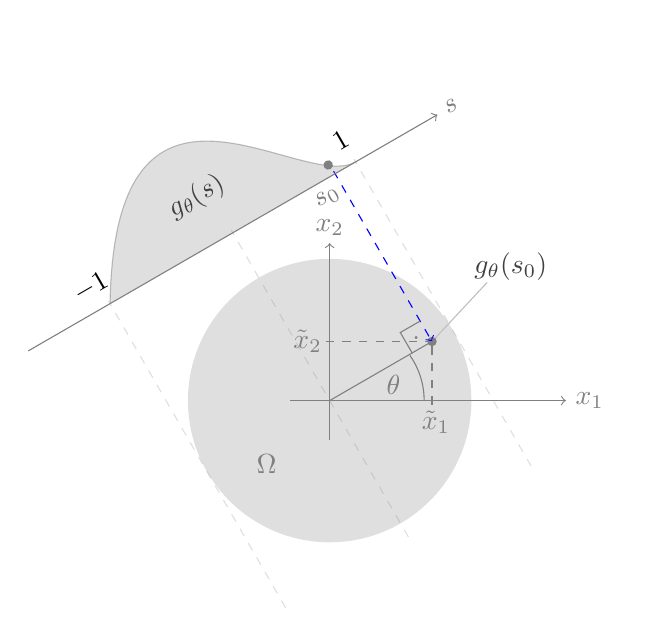
\begin{tikzpicture}	
	\fill[nearly transparent, color=gray] (0,0) circle (1.8cm);
	
	\draw [gray] [->](-0.5,0) -- (3,0); % x-Achse
	\draw [gray] (3, 0) node [right] {$x_1$};
	
	\draw [gray] [->](0,-0.5) -- (0,2); % y-Achse
	\draw [gray] (0, 2.2) node {$x_2$};
	
	\draw[lightgray](1.3,0.75) -- (2, 1.5);
	\fill[gray](1.3,0.75) circle [radius=0.06]; % ein Punkt		
	\draw [darkgray] (2.3, 1.7) node {$g_{\theta}(s_0)$};
	
	\draw [rotate=30, xshift=1.5cm, ->, dashed] [blue] (0,2.5) -- (0,0); % strahl
			
	
	\draw [xshift=1.05cm, yshift=0.6cm, rotate=120, - ] [gray] (0,0) -- (0.3,0);
	\draw [xshift=0.89cm, yshift=0.86cm, rotate=30, - ] [gray] (0,0) -- (0.3,0);
	\draw [gray] (1.1, 0.8)  node {$.$};
	
	\draw [rotate=30] [gray] [-] (0,0) -- (1.5, 0);
	
	\draw [dashed] [gray] (1.3,-0.05) -- (1.3,0.75); % x-Projektion
	\draw [gray] (1.35,-0.28)  node {$\tilde{x}_1$};
	
	\draw [dashed] [gray] (-0.05,0.75) -- (1.3,0.75); % y-Projektion		
	\draw [gray] (-0.28,0.75)  node {$\tilde{x}_2$};
	
	\draw [lightgray] [rotate=30, yshift=70] (-1.8,0) .. controls (0,3) and (1,0) .. (1.8,0);
	\fill [nearly transparent, color=gray] [rotate=30, yshift=70] (-1.8,0) .. controls (0,3) and (1,0) .. (1.8,0);

	\fill[ rotate=30, xshift=0.18cm, yshift=1.85cm, gray](1.3,0.75) circle [radius=0.06]; % ein Punkt
	
	\draw [rotate=30, xshift=0, yshift=70] [gray] [->] (-3,0) -- (3, 0);
	\draw [gray] (3.7, 0)  node [rotate=30, xshift=0, yshift=123] {$s$};
	
	\draw [gray] (0, 0)  node [rotate=30, xshift=1.55cm, yshift=2.25cm, left] {$s_0$};
	
	\draw [darkgray] (-0.2, 0)  node [rotate=30, yshift=85] {$g_{\theta}(s)$};		
	
	\draw [rotate=30, xshift=0cm, dashed] [nearly transparent, color=gray] (0,-2) -- (0,2.5); % punktiert Mitte
	\draw [rotate=30, xshift=1.8cm, dashed] [nearly transparent, color=gray] (0,-2) -- (0,2.5); % rechts punktiert
	\draw [rotate=30, xshift=-1.8cm, dashed] [nearly transparent, color=gray] (0,-2) -- (0,2.5); % links punktiert 
	
	\draw  (-1.8, 0) node [left, rotate=30, yshift=53]  {$-1$};
	\draw  (1.8, 0) node [right, rotate=30, yshift=105]  {$1$};
	
	\draw [gray] (1.2,0) arc [start angle=0, end angle=35, radius=1cm];
	\draw [gray] (0.6, 0.2) node [right] {$\theta$};
	
	\draw [gray] (-0.8, -0.8) node {$\Omega$};
	
	\end{tikzpicture}
	\caption{Ein Beispiel der Rückprojektion eines Projektionswerts $g_{\theta}(s_0)$ auf einen Punkt $x \in \Omega$. Mit $g_{\theta}(s)$ ist hier eine Projektion bei einem festen Winkel $\theta$ bezeichnet, also $g_{\theta}(s) = g(s,\theta)$.}
	\label{fig:1.7}
\end{figure}	  
\begin{proof}[Beweis von Lemma \ref{lemma:2}.]
Seien $f \in L^2(\Omega)$ und $g \in L^2(Z)$ beliebig, dann gilt
\begin{equation}
	\begin{split}
		\langle \mathcal{R} f, g \rangle_{L^2(Z)} & = \int\limits_{Z}^{} \left( \mathcal{R} f(s,\theta) \right) g(x^{T}\omega(\theta),\theta) \ \mbox{d}s \mbox{d}\theta \\
		& \stackrel{(\ref{equa:1.10})}{=} \int\limits_{0}^{\pi} \int\limits_{-1}^{1} \left( \int\limits_{-\gamma(s)}^{\gamma(s)}f(s\omega(\theta) + t\omega^{\perp}(\theta)) \mbox{d}t  \right) g(x^{T}\omega(\theta),\theta) \ \mbox{d}s \ \mbox{d}\theta.
		\end{split}
	\label{equa:1.23}
\end{equation}
An dieser Stelle machen wir eine Substitution in der rechten Seite von (\ref{equa:1.23}). Hier nutzen wir (\ref{equa:1.22}) aus und schreiben $x^T \omega(\theta) = \omega^T(\theta)x = s$. Dann bekommt man $g(x^{T}\omega(\theta),\theta) = g(\omega^T(\theta)x,\theta)$ und wir wollen die Funktion $f$ im Punkt $x$ betrachten, also $f(s\omega(\theta) + t\omega^{\perp}(\theta)) = f(x)$. Somit erhalten wir einen Integrationsbereich über $\Omega$. Nun führen wir (\ref{equa:1.24}) weiter:
\begin{equation}
	\begin{split}
		\langle \mathcal{R} f, g \rangle_{L^2(Z)} & = \int\limits_{0}^{\pi} \int\limits_{-1}^{1} \left( \int\limits_{-\gamma(s)}^{\gamma(s)}f(s\omega(\theta) + t\omega^{\perp}(\theta)) \mbox{d}t  \right) g(x^{T}\omega(\theta),\theta) \ \mbox{d}s \ \mbox{d}\theta \\
		& \stackrel{\mbox{\scriptsize Subst.}}{=}  \int\limits_{0}^{\pi} \left( \int\limits_{-1}^{1} \int\limits_{-\gamma(s)}^{\gamma(s)}f(x) g(\omega^T(\theta)x,\theta) \ \mbox{d}t \ \mbox{d}s \right) \mbox{d}\theta \\	
		& = \int\limits_{0}^{\pi} \int\limits_{\Omega} f(x) g(\omega^T(\theta)x,\theta) \ \mbox{d}x \ \mbox{d}\theta \\
		& = \int\limits_{\Omega} f(x) \left( \int\limits_{0}^{\pi} g(\omega^T(\theta)x,\theta) \ \mbox{d}\theta \right) \mbox{d}x  \\  
		& =\langle f, \mathcal{R^*} g \rangle_{L^2(\Omega)}.
	\end{split}
	\label{equa:1.24}
\end{equation}	 
Somit ist $\mathcal{R^*}$ adjungierter Operator der Radon Transformation und ist nach Satz von Schauder auch kompakt, wenn $\mathcal{R}$ kompakt ist. (\cite[S. 185]{Heuser75}).	 
\end{proof}

\subsubsection{Kompaktheit von $\mathcal{R}$}

Um die Kompaktheit von $\mathcal{R}$ zeigen zu können, werden wir an dieser Stelle einen Umweg einschlagen. Dafür ziehen wir ein Ergebnis aus \cite[S. 45]{Rieder03} heran. Es handelt sich um einen zu $\mathcal{R}$ adjungierten Operator $\tilde{\mathcal{R}}^*$ folgender Gestalt:
\begin{equation}
	\tilde{\mathcal{R}}^* : L^2(Z, \frac{1}{\gamma(s)}) \rightarrow L^2(\Omega).
	\label{equa:1.25}
\end{equation}
Hier wurde $\gamma(s)$ im Sinne der Gleichung (\ref{equa:1.8}) benutzt. Und der Raum $L^2(Z,\frac{1}{\gamma(s)})$ ist mit dem folgenden Skalarprodukt versehen
\begin{equation}
	\langle g,f \rangle = \int\limits_{Z} g \overline{f}\frac{1}{\gamma(s)}\mbox{d}s \mbox{d}\theta.
	\label{equa:1.26}
\end{equation}

Wir können festhalten dass der Operator $\mathcal{R'}:L^2(\Omega) \rightarrow  L^2(Z, \frac{1}{\gamma(s)})$ kompakt ist\footnote{Prinzipiell sind $\mathcal{R}$ und $\mathcal{R'}$ gleich, es ist derselbe Operator, der aber $L^2(\Omega)$ in einen anderen Raum abbildet. Die Bezeichnung $\mathcal{R}'$ führen wir ein, um uns Verwechslungen zu ersparen.}. Die Kompaktheit folgt eben aus der SWZ von $\mathcal{R}'$. Denn die Singulärwerte von $\mathcal{R}'$
\[
\sigma_j = 2\sqrt{\frac{\pi}{j + 1}}, \ \ j \in \N
\]
bilden eine Nullfolge, was nach einer längeren Rechnung aus \cite[S. 43]{Rieder03} folgt. Also schreiben wir $\mathcal{R}' \in \mathscr{K}(L^2(\Omega), L^2(Z,\frac{1}{\gamma(s)}))$\footnote{\label{foot:7}$\mathscr{K}(X,Y) = \{ A \in \mathscr{L}(X,Y) \ | \ A \mbox{ ist kompakt } \}$ }. 

Wir veranschaulichen die entstandene Situation in einem kommutativen Diagramm  
\begin{equation}
	\begin{xy}
	\xymatrix{
		L^2(\Omega) \ar[rr]^{\mathcal{R}} \ar@<2pt>[rd]^{\mathcal{R}'} &  & L^2(Z)\\
		&  L^2(Z, \frac{1}{\gamma(s)}) \ar@<2pt>[lu]^{\tilde{\mathcal{R}}^*} \ar[ru]_{\mbox{Id}}&
		}
	\end{xy}
	\label{equa:1.27}
\end{equation}
und stellen fest, dass $\mathcal{R}$ als eine Komposition zweier Abbildungen darstellbar ist. Hier bedeutet $\mbox{Id}$ die Identität auf $L^2(Z)$ dar. Der Unterschied zwischen $L^2(Z)$ und $L^2(Z,\frac{1}{\gamma(s)})$ besteht nur in der Definition des Skalarprodukts auf diesen beiden Räumen.

Insgesamt würde es heißen, dass wir die Komposition $\mbox{Id}\circ\mathcal{R}' = \mathcal{R}$ bezüglich der Kompaktheit beurteilen müssen. Dafür wird uns ein nützlicher Satz aus \cite[S. 27]{Rieder03} gute Dienste leisten (ohne Beweis) :
\begin{theorem}
	Seien $X, Y$ und $Z$ normierte Räume. Falls $A \in \mathscr{L}(X,Y)$ und $B \in \mathscr{K}(Y,Z)$ oder $A \in \mathscr{K}(X,Y)$ und $B \in \mathscr{L}(Y,Z)$, dann gilt $BA \in \mathscr{K}(X,Z)$.
	\label{satz:1}
\end{theorem}
Somit wollen wir zeigen, dass der Operator $\mbox{Id}:L^2(Z, \frac{1}{\gamma(s)}) \rightarrow L^2(Z)$ beschränkt ist, und somit auch stetig ist. Danach könnten wir den Satz \ref{satz:1} benutzen, um die Kompaktheit von $\mathcal{R}$ zu zeigen.

Sei nun $g(s,\theta) \in L^2(Z)$ beliebig, dann können wir folgende Abschätzung durchführen:
\begin{equation}
	\begin{split}
		\parallel \mbox{Id} \ g(s, \theta) \parallel_{L^2(Z)}^{2} & = \ \int \limits_{Z} |\mathcal{R}f(s, \theta)|^2 \mbox{d}s \mbox{d}\theta \\
		& \stackrel{(\ref{equa:1.26})}{\leq} \int \limits_{Z}  |\mathcal{R}f(s, \theta)|^2 \frac{1}{\gamma(s)} \ \mbox{d}s \ \mbox{d}\theta\\
		& = \ \parallel g(s, \theta) \parallel_{L^2(Z, \frac{1}{\gamma(s)})}^{2}.
	\end{split}
	\label{equa:1.28}
\end{equation}
Die letzte Abschätzung beruht auf der Kenntnis, dass  $\gamma(s) \leq 1$ für alle $s \in (-1,1)$, somit aber $\frac{1}{\gamma(s)} \geq 1$ gilt. Nun haben wir gezeigt, dass $\parallel \mbox{Id} \parallel_2 \leq 1$ beschränkt und demnach stetig ist. Also gilt $\mbox{Id} \in \mathscr{L}(L^2(Z, \frac{1}{\gamma(s)}), L^2(Z))$. Dieses Ergebnis ist für uns ausreichend um den Satz \ref{satz:1} benutzen zu können, d.h 
\begin{equation}
	\mathcal{R} \stackrel{(\ref{equa:1.27})}{=} \mbox{Id} \circ \mathcal{R}' \xLongrightarrow{\text{Satz \ref{satz:1}}} \mathcal{R} \in \mathscr{K}(L^2(\Omega), L^2(Z)).
	\label{equa:1.29}
\end{equation}

Nun sind wir am Ende dieses Kapitels angelangt und nach einigen Untersuchungen können wir festhalten, dass der lineare stetige Operator $\mathcal{R} : L^2(\Omega) \rightarrow L^2(Z)$ kompakt ist und einen kompakten adjungierten Operator $\mathcal{R^*}$ hat. Diese Ergebnisse spielen eine zentrale Rolle bei der Singulärwertzerlegung (SWZ) eines kompakten Operators und beleuchten das Problem der Invertierung solcher Operatoren sehr gut.

\subsubsection{Die Singulärwertzerlegung (SWZ) von $\mathcal{R}$}

Im Folgenden wird die allgemeine Form der SWZ des Operators $\mathcal{R}$ angegeben, eine konkrete wird in \cite[Kap. 2.5]{Rieder03} hergeleitet, jedoch aber nur für $\mathcal{R}'$. Um zu SWZ von $\mathcal{R}$ zu gelangen, ermittelt man zuerst die Eigenwerte und Eigenvektoren von $\mathcal{R}\mathcal{R^*} : L^2(Z) \rightarrow L^2(Z)$, die als Komposition kompakter Operatoren kompakt ist. Demnach gilt der \textit{Spektralsatz für selbstadjungierte kompakte Operatoren} \cite[S. 30]{Rieder03} und man bekommt 
\begin{equation}
	\mathcal{R}\mathcal{R^*}g = \sum\limits_{j=1}^{\infty} \lambda_j \langle g, v_j \rangle_{L^2(Z)} v_j, \ \ \mbox{für alle} \ \ g \in L^2(Z).
	\label{equa:1.30}
\end{equation}
Hier bildet $\{ \lambda_j \}_{j \in \N} \in \R$ eine Folge mit der absteigenden Anordnung der Eigenwerte $|\lambda_1| \geq |\lambda_2| \geq ... > 0$ und $\{ v_j\}_{j \in \N} \in L^2(Z)$ ein Orthonormalsystem in $\mbox{Kern}(\mathcal{R})^{\perp}$. Eine wichtige Tatsache ist, dass die Folge $\{\lambda_j\}_{j \in \N}$ entweder abbricht oder gegen Null konvergiert.

Die Singulärwerte und das Orthonormalsystem $\{u_j\}_{j \in \N}$ des Bildes von $\mathcal{R}$ bekommen wir aus
\begin{equation}
	\begin{split}
		(i). \ \sigma_j &:= \sqrt{\lambda_j}\\ 
		(ii). \ u_j	&:= \sigma_j^{-1}\mathcal{R}v_j
	\end{split}
	 , \ \  j \in \N.
	 \label{equa:1.31}
\end{equation}
Mit den Ergebnissen aus (\ref{equa:1.30}) und (\ref{equa:1.31}) kann nun die SWZ der Radon Transformation angegeben werden
\begin{equation}
	\mathcal{R}f = \sum\limits_{j = 1}^{\infty} \sigma_j \langle f, v_j\rangle_{L^2(\Omega)} u_j.
	\label{equa:1.32}
\end{equation}
Das Tripel $\{(\sigma_j, v_j, u_j)\}$ nennt man \textit{Singulärsystem} eines kompakten Operators und die Folgen $\{u_j\}_{j \in \N}$ und $\{ v_j\}_{j \in \N}$ bilden folgende Orthonormalsysteme
\begin{equation}
	\overline{\mbox{Span}\{u_j | j \in \N \} } = \overline{\mbox{Bild}(\mathcal{R})} \ \ \mbox{und} \ \ \overline{\mbox{Span}\{v_j | j \in \N \} } = \mbox{Kern}(\mathcal{R})^{\perp}.
	\label{equa:1.33}
\end{equation}

Die Gleichung (\ref{equa:1.32}) wird im nächsten Kapitel bei der Klärung des Begriffs \textit{schlecht gestellter Probleme} sehr hilfreich sein. 







		\include{captures/Inverse_Probleme}
		\chapter*{Rekonstruktionsverfahren und ihre Implementierung}
\label{cha:3}

In diesem Kapitel werden wir die praktische Vorgehensweise einiger Bildrekonstruktionstechniken in der Computertomographie diskutieren. Den Stützpunkt folgender Diskussion werden wir zuerst hier festigen. Dazu schauen wir uns nochmal das diskrete Modell (\ref{equa:2.2}) an:

\[\mathcal{R}f = \sum\limits_{j = 1}^{n} \sigma_j \langle f, v_j\rangle_{L^2(\Omega)} u_j, \ \ n \in \N.\] 

Die obige Gleichung stellt genau $n$ Projektionen $p \in \R^n$ einer unbekannten Dichtefunktion $f \in \R^m$ dar. Die Anzahl der Projektionen $n$ setzt sich aus der Anzahl der Detektorzellen $k \in  \N$ im Detektorband und der Anzahl der Winkel $q \in \N$ zu denen die Projektionen erzeugt worden sind zusammen. Insgesamt ergibt sich
\begin{equation}
	n = kq \ \ \mbox{für} \ n,k,q \in \N.
	\label{equa:3.1}
\end{equation}
\begin{figure}[H]
	\centering
	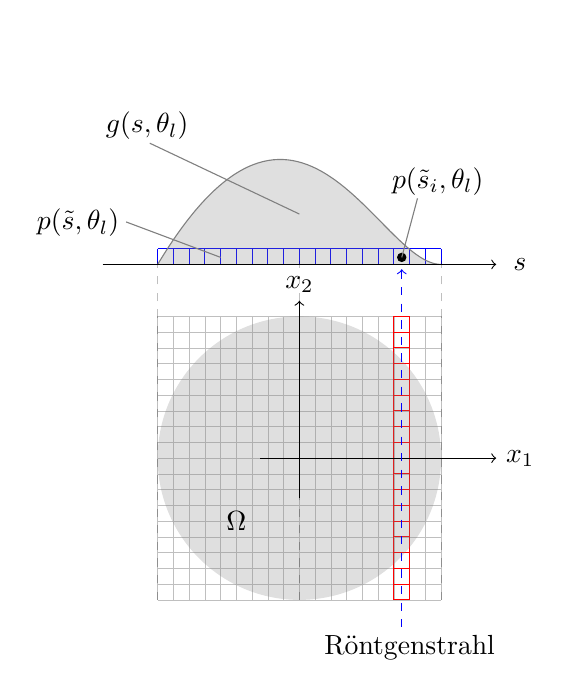
\begin{tikzpicture}
	
	\draw [step=0.2,blue, thin, rotate=0, xshift=0, yshift=70] (-1.8,0) grid (1.8,0.2); % detector grid
	
	\draw [step=0.2, lightgray, very thin] (-1.8,-1.8) grid (1.8,1.8); % picture grid
	
	\draw [step=0.2, red, thin, rotate=0, xshift=1.2cm, yshift=0] (0,-1.8) grid (0.2,1.8);
	
	\fill[nearly transparent, color=gray] (0,0) circle (1.8cm);
	
	\draw [black] [->](-0.5,0) -- (2.5,0); % x-Achse
	\draw [black] (2.5, 0) node [right] {$x_1$};
	
	\draw [black] [->](0,-0.5) -- (0,2); % y-Achse
	\draw [black] (0, 2.2) node {$x_2$};
	
	\draw [rotate=0, xshift=1.3cm, <-, dashed] [blue] (0,2.4) -- (0,-2.2); % strahl
	\draw [black] (1.4, -2.4) node {Röntgenstrahl};
	
	\draw [gray] [rotate=0, yshift=70] (-1.8,0) .. controls (0,3) and (1,0) .. (1.8,0);
	\fill [nearly transparent, color=gray] [rotate=0, yshift=70] (-1.8,0) .. controls (0,3) and (1,0) .. (1.8,0);
	
	\fill[ rotate=0, xshift=0cm, yshift=1.8cm, black](1.3,0.75) circle [radius=0.06]; % ein Punkt
	
	\draw [rotate=0, xshift=0, yshift=70] [black] [->] (-2.5,0) -- (2.5, 0);
	\draw [black] (2.8, 0)  node [rotate=0, xshift=0, yshift=70] {$s$};
	
	\draw [black] (0, 0)  node [rotate=0, xshift=-80, yshift=85] {$p(\tilde{s}, \theta_l)$};
	\draw[gray,  yshift=1.8cm](-1,0.75) -- (-2.2, 1.2);	
	
	\draw [black] (0, 0)  node [rotate=0, xshift=50, yshift=100] {$p(\tilde{s}_i, \theta_l)$};
	\draw[gray,  yshift=1.8cm](1.3,0.75) -- (1.5, 1.5);		
	
	\draw [black] (0, 0)  node [rotate=0, xshift=-55, yshift=120] {$g(s, \theta_l)$};
	\draw[gray,  yshift=1.8cm](0,1.3) -- (-1.9, 2.2);		
	
	\draw [rotate=0, xshift=0cm, dashed] [nearly transparent, color=black] (0,-1.8) -- (0,2.5); % punktiert Mitte
	\draw [rotate=0, xshift=1.8cm, dashed] [nearly transparent, color=black] (0,-1.8) -- (0,2.5); % rechts punktiert
	\draw [rotate=0, xshift=-1.8cm, dashed] [nearly transparent, color=black] (0,-1.8) -- (0,2.5); % links punktiert 
	
	\draw [black] (-0.8, -0.8) node {$\Omega$};
	
	\end{tikzpicture}
	\caption{Anschauliche Darstellung der Diskretisierung der Dichtefunktion $f$. Entlang des Röntgenstrahls (alle rot umrandeten Pixel) an der Stelle $s_i$ und zu einem festen Winkel $\theta_l = 0$, werden die Werte von $f$ zu dem Wert $p(\tilde{s}_i, \theta_l)$ aufsummiert. $p(\tilde{s}, \theta_l)$ ist der Vektor zu allen Strahlen an den Stellen $\tilde{s}_i$ und somit die Diskretisierung von $g(s,\theta_l)$.}
	\label{fig:3.1}
\end{figure}
Die Diskretisierung von $f$ hängt hingegen nur von der Anzahl der Detektorzellen $k \in \N$ im Detektorband ab. Betrachtet man die Abbildung \ref{fig:3.1}, dann wird man erkennen, dass die $k$ Detektorzellen die Breite und die Höhe des zu rekonstruierenden Bildes $f$ festlegen, demnach ergibt sich
\begin{equation}
	m = k^2 \ \ \mbox{für} \ k, m \in \N.
	\label{equa:3.2}
\end{equation}
\begin{Bemerkung}
	Praktisch gesehen, stellt $k$ die Anzahl der digitalen Pixel in der Breite und Tiefe eines digitalen Bildes $f$ dar.
	\label{bem:6}
\end{Bemerkung}
Bevor wir im nächsten Schritt zur Bildrekonstruktion übergehen, schauen wir uns zuerst die Entstehung der Projektionsdaten aus der Radon Transformation etwas genauer an. Betrachten wir dazu die Gleichung (\ref{equa:1.10}) und die Abbildung \ref{fig:1.6}.
\[ \mathcal{R}f(s,\theta) = \int\limits_{-\gamma(s)}^{\gamma(s)} f(s\omega(\theta) + t\omega^{\perp}(\theta))\mbox{d}t. \]
Im diskreten Fall $\tilde{f} \in \R^{k \times k}$ wird man feststellen, dass (\ref{equa:1.10}) die Summe aller Werte von $\tilde{f}$ entlang einer Geraden $G$, den Projektionswert $p(\tilde{s}_i, \theta_l)$ an der Stelle $\tilde{s}_i, i \in [1,k]$, entsprechend dem Winkel $\theta_l, \ l \in [1,q] $, liefert. Damit kann (\ref{equa:1.10}) für die Transformation eines digitalen Bildes folgendermaßen interpretiert werden
\begin{equation}
	\begin{split}
		p(\tilde{s}_i, \theta_l) & = \sum \limits_{j = 1}^{m} \mu_j \Delta\tilde{t}, \ \mbox{mit} \ m = k^2, \\
		\mbox{für} \ \mu_j & = \left\{ \begin{matrix}
							\tilde{f}_j & : & \mbox{falls } \tilde{f}_j\cap G \neq \emptyset \\ 
							0 & : & \mbox{sonst}
						\end{matrix}.\right.
	\end{split}
	\label{equa:3.3}
\end{equation}

Fasst man auf diese Weise zu jedem $\tilde{s}_i$ (wobei $\Delta\tilde{t} = 1$) die entsprechende Werte von $\tilde{f}$ zusammen, so entsteht der Projektionsvektor $p(\tilde{s},\theta_l)$ (Abb. \ref{fig:3.1}). Stellt man alle Projektionen $p(\tilde{s}, \theta_l)$ entsprechend der Winkelreihenfolge $\theta_l, \ l \in [1,q]$ auf, so entsteht ein digitales Bild der Projektionsdaten der diskreten Radon Transformation.
\begin{Bemerkung}
	Die Gleichung (\ref{equa:3.3}) entspricht der Parallelstrahlengeometrie. Das bedeutet, dass alle Geraden $G$, die das Objekt durchdringen, parallel zueinander sind. Um (\ref{equa:3.3}) in die Fächerstrahlengeometrie zu überführen, müssen entsprechende geometrische Transformationen durchgeführt werden.
	\label{bem:7}
\end{Bemerkung}

Schauen wir uns ein konkretes Beispiel einer Radon Transformation an. Sei dazu die Abbildung \ref{fig:3.2} betrachtet. In Abb. \ref{fig:3.2.b} ist die Radontransformierte oder \textit{das Sinogramm} von Abb. \ref{fig:3.2.a} gemäß (\ref{equa:3.3}) zu sehen. Der Aufbau des Sinogramms entspricht dem oben beschriebenen Prinzip. Fasst man also das Sinogramm in Abb. \ref{fig:3.2.b} als eine Matrix auf, so ist jede Spalte der Matrix gleich einer Projektion $g(\tilde{s}, \theta_l)$ zu einem festem Winkel $\theta_l$. Die Implementierung der (diskreten) Radon Transformation ist im Abschnitt \ref{cha:A.1} kurz erläutert.
\begin{figure}[H]
	\begin{center}
		\subfloat[\label{fig:3.2.a}Phantombild]{{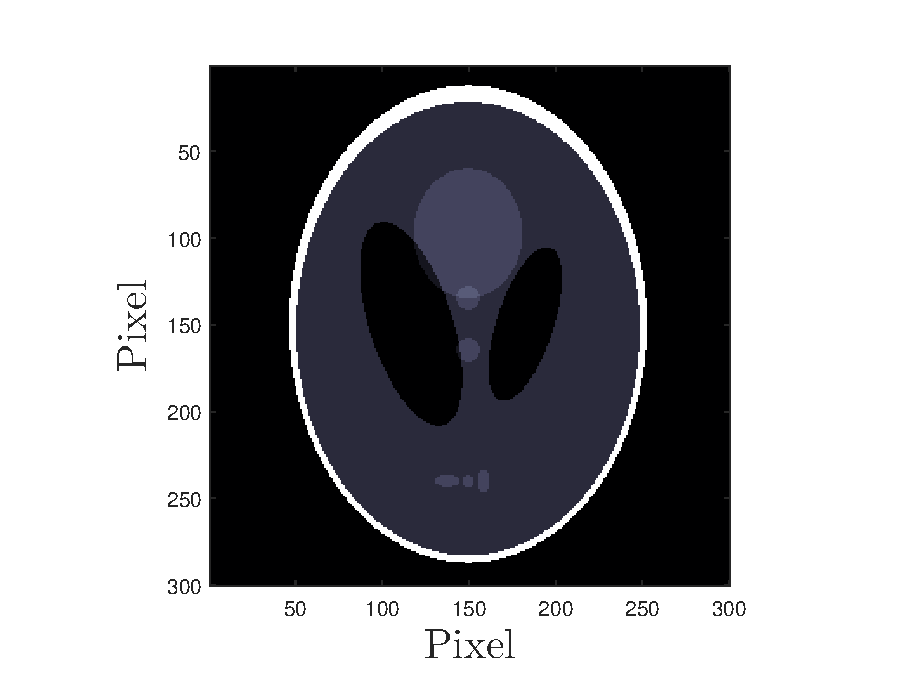
\includegraphics[width=0.5\textwidth]{phantom.eps} }}
		\subfloat[\label{fig:3.2.b}Die Radon Transformation des Phantombildes]{{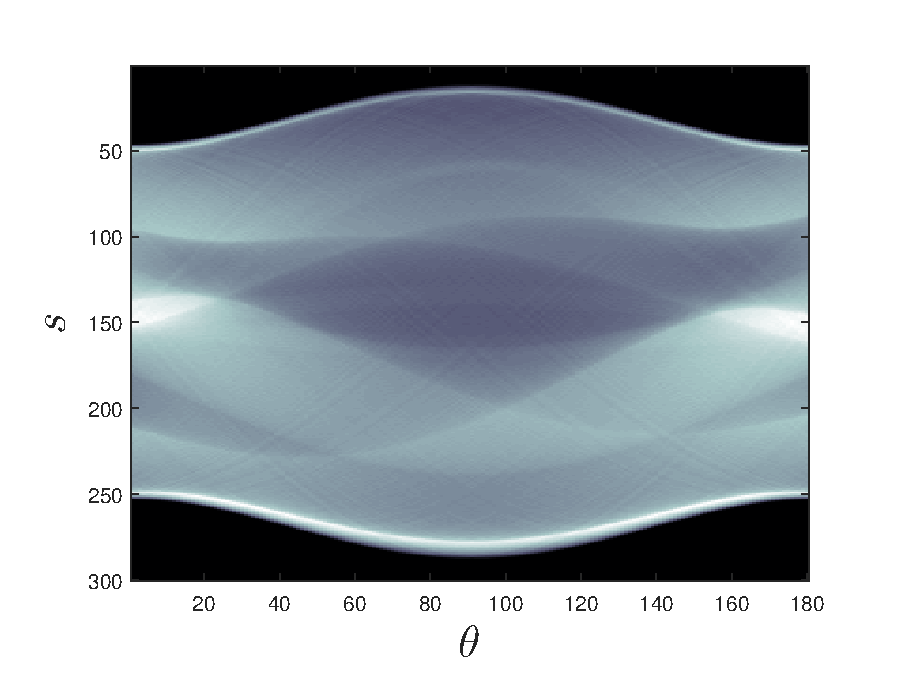
\includegraphics[width=0.5\textwidth]{rt_phantom.eps} }}
	\end{center}
	\caption{ Links (a) ist ein Phantombild (Quelle: \MATLAB, \texttt{\captionstring phantom(300)}) zu sehen, welches wir für alle Testzwecke in diesem Kapitel benutzen werden. Rechts (b) ist die Radontransformierte von (a) abgebildet. Die Transformation wurde über $\theta \in [0^{\circ}, 180^{\circ}]$ mit einer Schrittweite von $1^{\circ}$ durchgeführt. Das Detektorband hat eine Länge von $k = 300$, wobei $k$ gleich der Anzahl der Tiefenpixel von (a) ist. Somit bestimmt $k$ auch die Anzahl der Strahlen, die durch das Phantombild geschickt worden sind.}
	\label{fig:3.2}
\end{figure}

Sinogramme sind in der Praxis der computertomographischen Bildrekonstruktion genau die gemessenen Daten. Somit ist die Aufgabe das Bild des Ursprungsobjekts aus einem Sinogramm zu rekonstruieren. In folgenden Abschnitten werden wir uns vier solcher Rekonstruktionsverfahren anschauen. Dabei unterscheiden wir zwischen \textit{analytischen} und \textit{algebraischen} Verfahren. Als Nächstes wollen wir den Begriff der analytischen Rekonstruktion klären.

\section*{Analytische Rekonstruktionsverfahren}
\label{cha:3.1}

Der Begriff der \textit{analytischen Rekonstruktion} bedeutet in diesem Fall, dass die Algorithmen der CT-Bildrekonstruktion direkt aus den analytischen Formeln hergeleitet werden. Solche Verfahren nutzen die Projektionsdaten zur Rekonstruktion des Bildes direkt aus. Zuerst schauen wir uns das einfachste davon an.

\subsection*{Ungefilterte Rückprojektion}
\label{cha:3.1.1}

Den Ausgangspunkt dieses Abschnitts liefert uns der Adjungierte Operator (\ref{equa:1.21}). Schauen wir uns die Gleichung des Operators $\mathcal{R}^*$ noch einmal an: 

\[ \mathcal{R^*} g(x) = \int\limits_{0}^{\pi} \ g(x^{T}\omega(\theta),\theta) \mbox{d}\theta. \]  

Aus der Bemerkung \ref{bem:3} wissen wir bereits, dass (\ref{equa:1.21}) die ungefilterte Rückprojektion darstellt. Das Argument des Integranden in der obigen Gleichung ist ein fester Punkt $x$ der Kreisscheibe $\Omega$. Auf diesen Punkt $x$ wird aus allen Winkeln zurück projiziert. Führt man das für alle $x \in \Omega$ durch, so entsteht ein verschwommenes Bild des Originals, wie es die Abbildung \ref{fig:3.3.b} zeigt.
\begin{figure}[!h]
	\begin{center}
		\subfloat[\label{fig:3.3.a}Die Radon Transformation des Phantombildes aus Abb. \ref{fig:3.2.a}.]{{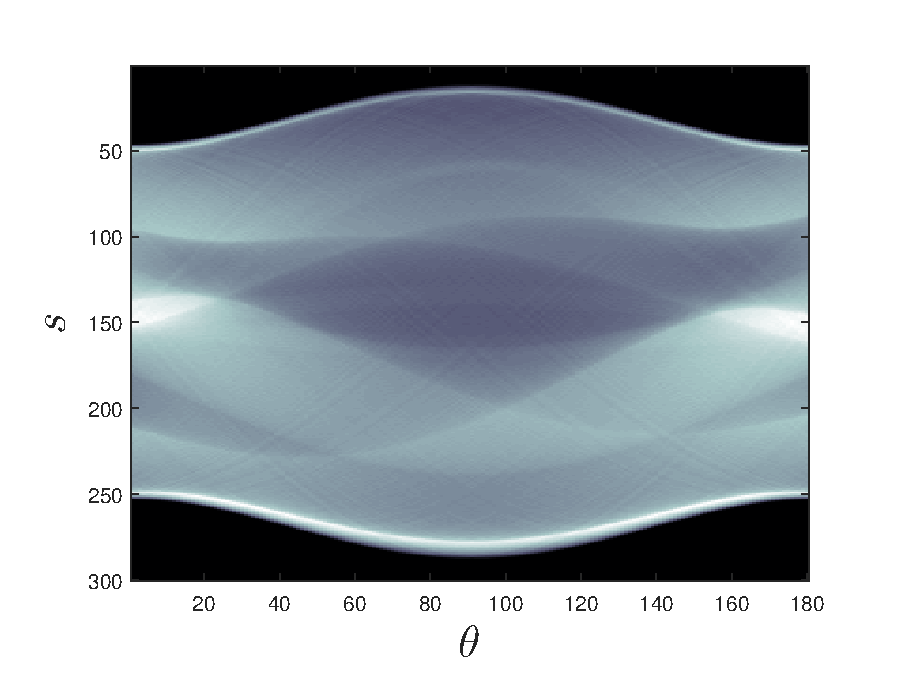
\includegraphics[width=0.5\textwidth]{rt_phantom.eps} }}
 		\subfloat[\label{fig:3.3.b}Ungefilterte Rückprojektion]{{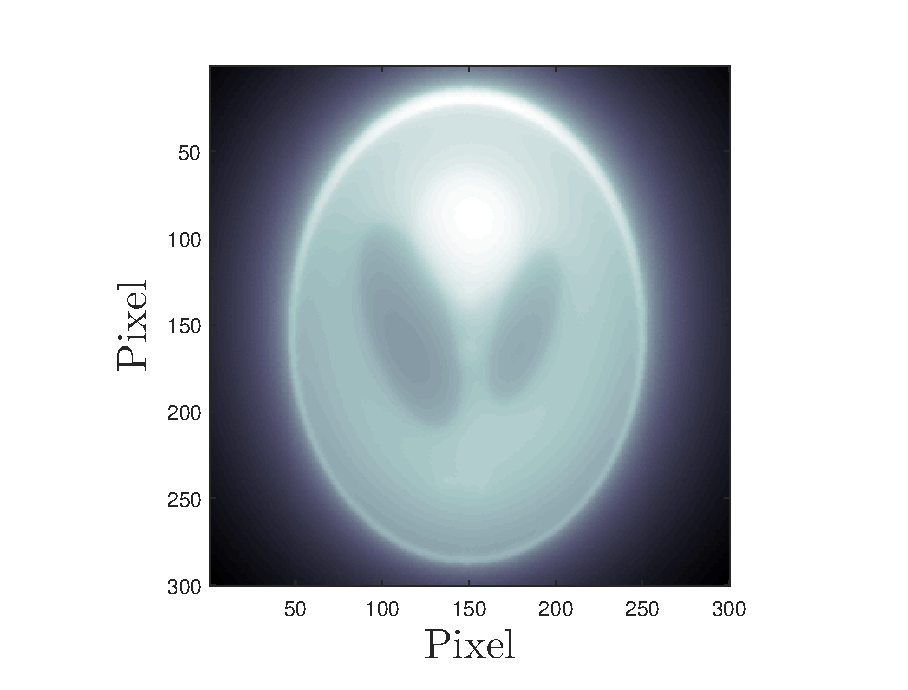
\includegraphics[width=0.5\textwidth]{backProjection.eps} }}
	\end{center}
	\caption{ Links (a) ist die Radontransformierte wie in der Abb. \ref{fig:3.2.b}. Rechts (b) ist die ungefilterte Rückprojektion von (b).}
	\label{fig:3.3}
\end{figure}

Jetzt wollen wir nachvollziehen, warum der Effekt der Verschwommenheit bei der ungefilterten Rückprojektion auftritt. Dazu sei zunächst die Abbildung \ref{fig:3.4} betrachtet, denn mit ihrer Hilfe können wir den Zusammenhang zweier Punkte in der Ebene $\Omega$ nachvollziehen.
\begin{figure}[H]
	\begin{minipage}[t]{0.4\textwidth}
		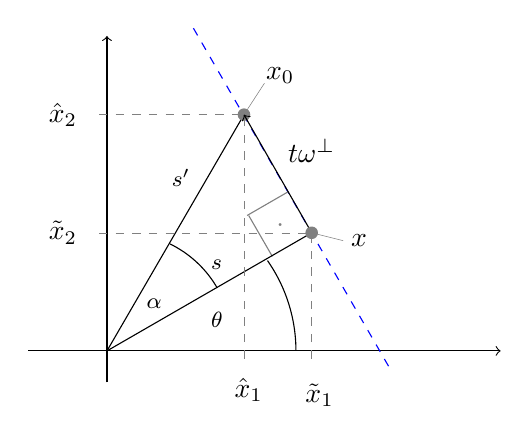
\begin{tikzpicture}[scale=2]		
			\draw [black] [->](-0.5,0) -- (2.5,0); % x-Achse
			\draw [black] [->](0,-0.2) -- (0,2); % y-Achse
			
			\draw [rotate=30, xshift=1.5cm, dashed] [blue] (0,1.5) -- (0,-1); % strahl
			
			\draw [xshift=1.05cm, yshift=0.6cm, rotate=120, - ] [gray] (0,0) -- (0.3,0);
			\draw [xshift=0.89cm, yshift=0.86cm, rotate=30, - ] [gray] (0,0) -- (0.3,0);
			\draw [gray] (1.1, 0.8)  node {$.$};
			
			\draw [black] [-] (0,0) -- (1.3,0.75); % s line
			\draw [black] (0.35, 1.1) node [right] {\footnotesize$s'$}; % s'
			\draw [dashed, very thin] [gray] (0.87,-0.05) -- (0.87,1.5); % \hat{x1} Projektion
			\draw [black] (0.9,-0.25)  node {$\hat{x}_1$};
			
			\draw [black] [-] (0,0) -- (0.87,1.5); % s' line
			\draw [black] (0.6, 0.55) node [right] {\footnotesize$s$}; % s
			\draw [dashed, very thin] [gray] (-0.05,1.5) -- (0.87,1.5); % \hat{x2} Projektion
			\draw [black] (-0.28,1.5)  node {$\hat{x}_2$};
			
			\fill[gray](0.87,1.5) circle [radius=0.04]; %x point 
			\draw[gray, very thin](0.87,1.5) -- (1, 1.7);
			\draw [black] (1.1, 1.75) node {$x_0$};
			
			\draw [black] [->] (1.3,0.75) -- (0.87,1.5); % t line
			\draw [black] (1.3,1.27) node {$t\omega^{\perp}$};	
			
			\fill[gray](1.3,0.75) circle [radius=0.04];
			\draw[gray, very thin](1.3,0.75) -- (1.5, 0.7);
			\draw [black] (1.6, 0.7) node {$x$};
			
			\draw [dashed, very thin] [gray] (1.3,-0.05) -- (1.3,0.75); % x-Projektion
			\draw [black] (1.35,-0.28)  node {$\tilde{x}_1$}; %\tilde{x1}
			
			\draw [dashed, very thin] [gray] (-0.05,0.75) -- (1.3,0.75); % y-Projektion		
			\draw [black] (-0.28,0.75)  node {$\tilde{x}_2$}; % \tilde{x2}
			
			\draw [black] (1.2,0) arc [start angle=0, end angle=35, radius=1cm]; % angle \theta
			\draw [black] (0.6, 0.2) node [right] {\footnotesize$\theta$};
			
			\draw [black] (0.7,0.4) arc [start angle=30, end angle=64, radius=0.7cm];
			\draw [black] (0.3, 0.3) node {\footnotesize$\alpha$};
		
		\end{tikzpicture}		
	\end{minipage}
	\begin{minipage}[b][5cm][t]{0.6\textwidth}
		\begin{align}
			& \beta = \alpha + \theta \label{equa:3.4}\\
			& x = \left(\begin{array}{c} \tilde{x_1} \\ \tilde{x_2} \end{array}\right) = s \left(\begin{array}{c} \cos(\theta) \\ \sin(\theta) \end{array}\right) = s\omega(\theta) \label{equa:3.5}\\
			& x_0 = \left(\begin{array}{c} \hat{x_1} \\ \hat{x_2} \end{array}\right) = s' \left(\begin{array}{c} \cos(\beta) \\ \sin(\beta) \end{array}\right) = s'\omega(\beta) \label{equa:3.6}\\
			& s'\omega(\beta) = s\omega(\theta) + t\omega^{\perp}(\theta)
			\label{equa:3.7}
		\end{align}
	\end{minipage}
	\caption{Eine Skizze (links) zur Verdeutlichung der Beziehung zweier Punkte $x_, x_0 \in \Omega$ bezüglich ihrer kartesischen- und Polar-Koordinaten. Die dazugehörige Nebenrechnung (rechts) zeigt deren formelmäßigen Zusammenhang auf.}
	\label{fig:3.4}
\end{figure}

Hier ist das Ziel zu zeigen dass, dass die ungefilterte Rückprojektion eine Faltung von $f(x) , \ x \in \Omega$ mit einer noch näher zu bestimmenden Funktion $h(x), \ x \in \Omega$ darstellt. Dazu formulieren wir folgendes Lemma:
\begin{lemma}
	Sei $f(x) \in L^2(\Omega)$ beliebig und $h(x) \in L^2(\Omega)$ speziell, dann kann die ungefilterte Rückprojektion als Faltung zweier Funktionen als
	\[ \mathcal{R^*} g(x_0) = \int \limits_{\R^2} f(x)h(x-x_0) \mbox{d}x = f(x)*h(x).\]	
	geschrieben werden. Da $\mbox{supp}f \subset \Omega$ betrachten wir das obige Integral nur auf $\Omega$.
	\label{lemma:3}
\end{lemma}
\begin{Bemerkung}
	Bevor wir zum Beweis übergehen, führen wir die dafür benötigte $\delta$-Distribution und einige für uns nützliche Eigenschaften ein. Seien $x, x_0 \in \R^2$, dann gilt:
	\begin{align}
	   	&  \ \  \delta(x-x_0) = \left\{ \begin{matrix} 0 & : &  x \neq x_0 \\ \infty & : & x = x_0 \end{matrix}\right. \label{equa:3.8}
   	\end{align}
	Eigenschaften :
	\begin{align}
		(\lowroman{1}).  &  \ \ \langle \delta(x-x_0), f(x)\rangle = \int \limits_{-\infty}^{\infty} f(x)\delta(x-x_0)\mbox{d}x = f(x_0) \label{equa:3.9}\\
		(\lowroman{2}). &  \ \  \delta(ax) = \frac{1}{|a|}\delta(x) \label{equa:3.10} \\
		(\lowroman{3}). &  \ \  \int \limits_{-\infty}^{-\infty}\delta(x-x_0) \mbox{d}x = 1 \label{equa:3.11}
	\end{align}
	\label{bem:8}
\end{Bemerkung}
\begin{proof}
	Wir Beginen mit der Definition der ungefilterten Rückprojektion (\ref{equa:1.21}) und benutzen dabei die Nebenrechnung zu Abb. \ref{fig:3.4} sowie die eingeführten Eigenschaften der $\delta$-Distribution aus der Bemerkung \ref{bem:8}.
	\begin{equation}
	\begin{split}
		\mathcal{R^*} g(x_0) & = \int\limits_{0}^{\pi} \ g(x_{0}^{T}\omega(\theta),\theta) \ \mbox{d}\theta  \ \  \stackrel{(\ref{equa:1.10}, \ \ref{equa:3.7})}{=} \ \ \int\limits_{0}^{\pi} \left( \int\limits_{-\gamma(s)}^{\gamma(s)} f(s'\omega(\beta)) \ \mbox{d}t \right) \mbox{d}\theta \\
		& \stackrel{(\ref{equa:3.9})}{=} \int\limits_{0}^{\pi} \left( \int\limits_{-\gamma(s)}^{\gamma(s)} \int\limits_{-1}^{1} f(s\omega(\theta)) \delta(s\omega(\theta) - s'\omega(\beta)) \ \mbox{d}s \ \mbox{d}t \right) \mbox{d}\theta \\
		& \stackrel{(\ref{equa:3.7})}{=} \int\limits_{0}^{\pi} \left( \int\limits_{\Omega} f(x) \delta(t\omega^{\perp}(\theta)) \ \mbox{d}x \right) \mbox{d}\theta \stackrel{(\ref{equa:3.10})}{=} \int\limits_{\Omega} f(x) \frac{\int\limits_{0}^{\pi}\delta(\beta - \alpha)\mbox{d}\beta}{|t\frac{\partial \omega^{\perp}(\theta)}{\partial \theta}|} \mbox{d}x \\
		& \stackrel{(\ref{equa:3.11})}{=} \int\limits_{\Omega} f(x) \frac{1}{|x - x_0|} \mbox{d}x = f(x)*h(x).
	\end{split}
	\label{equa:3.12}
	\end{equation}
	In der letzten Zeile wurde $|t\frac{\partial \omega^{\perp}(\theta)}{\partial \theta}| = |t||\left(\begin{array}{c} -\cos(\theta) \\ -\sin(\theta) \end{array}\right)| = |t| = |x -x_0|$ benutzt.
\end{proof}
Somit haben wir auch die spezielle Funktion $h(x) = \frac{1}{|x|}$ gefunden. Die Funktion $h$ heißt \textit{Point-Spread-Function}. Anschaulich kann $f$ in jedem Punkt als $\delta$-Distribution verstanden werden. Das heißt, setzt man $f$ auf ganz $\Omega$ Null, außer im Punkt $x_0 \in \Omega$ und faltet mit $h(x)$, so wird das Ergebnis $\tilde{f}$ um den Punkt $x_0$ nach außen radial abfallen. Führt man die Faltung von $f$ für jeden Punkt in $\Omega$ und setzt auf diese Weise entstandene Faltungsbilder zusammen führt das zu dem Effekt der Verschwommenheit. 

\subsection*{Gefilterte Rückprojektion}
\label{cha:3.1.2}

Das in dem letzten Abschnitt erreichte Ergebnis ist für die Praxis unbrauchbar. Man kann an einem verschwommenen Bild keine qualitative Analyse durchführen. Deshalb werden wir in diesem Abschnitt eine Verbesserung des ersten Verfahrens suchen. Wie der Name schon verrät, bekommt man ein ungefiltertes Bild zurück. Wir wollen nun verstehen, wie man die Projektionsdaten filtert, bevor man sie zurück projiziert.

Um den Ausdruck der \textit{gefilterten Rückprojektion} zu bekommen, werden wir uns des sogenannten \textit{Fourier\footnote{Jean Baptiste Joseph Fourier (1768 - 1830) ein französischer Mathematiker und Physiker.}-Slice-Theorem} (FST) bedienen (siehe z.B. \cite[S. 120]{Buzug04}). Das Schema des Theorems kann nun folgendermaßen wiedergegeben werden:
\begin{enumerate}
	\item Berechne für einen festen Winkel $\theta$ die Fouriertransformierte\footnote{
		\label{foot:14}\textbf{Definition }\textit{Fourier-Transformation}. Sei $f(x) \in L^2(\Omega)$, dann ist ihre Fourier-Transformation durch
			\begin{equation}
				(\mathcal{F}f)(x) = \int \limits_{\Omega} f(x) e^{-2\pi i \langle x^T, u \rangle} \mbox{d}x = F(u), \ \ u \in \mathbb{C}^2
				\label{equa:3.13}
			\end{equation}
		gegeben.} (FT) einer Projektion $\mathcal{R}f(s,\theta) = g(s,\theta)$
	\[(\mathcal{F}g)(s,\theta) = G(q, \theta). \]
	\item Konstruiere die Fouriertransformierte $F(u,v)$ von $f(x)$ aus $G(q,\theta)$
	\[G(q,\theta) \leadsto F(u).\]
	\item Berechne die inverse Fouriertransformierte von $F$
	\[(\mathcal{F}^{-1}F)(u) = \tilde{f}(x). \]
\end{enumerate}

Wir werden den Punkt 2 des FST vom Punkt 1 und dann vom Punkt 3 aus schrittweise annähern. Bevor wir die Herleitung der gefilterten Rückprojektion angehen, machen wir uns die vorliegende Situation an einer Skizze (Abb. \ref{fig:3.5}) klar. 

In der Abbildung \ref{fig:3.5} ist schematisch wiedergegeben, dass die Fourier-Transformation an der Natur der Koordinatensysteme nichts ändert. Diese Tatsache wird in dem \textit{Plancherel-Theorem} bewiesen, welches unter anderem besagt, dass die die FT ein \text{unitärer} Operator für Funktionen aus $L^2$ ist. Das heißt, die FT ist linear, isometrisch und bijektiv. Das weiteren beweist der Satz die Invertierbarkeit von $\mathcal{F}$ für $L^2$ Funktionen. 
\begin{figure}[!h]
	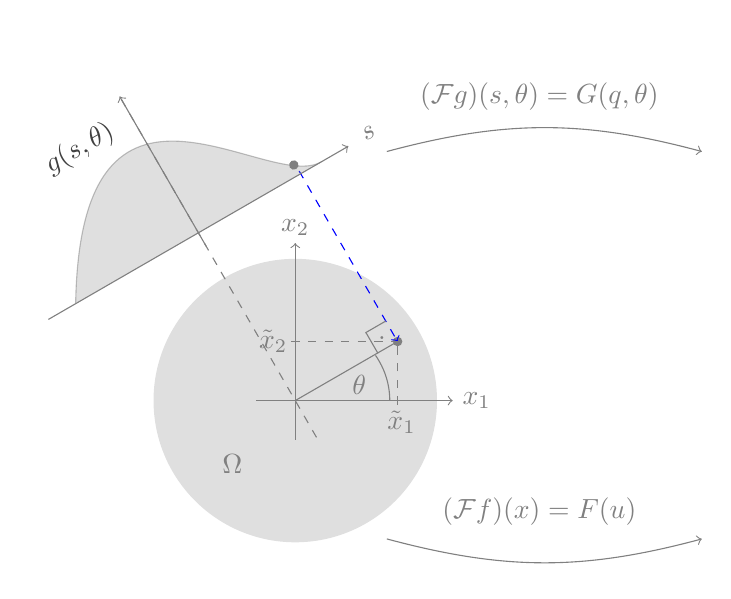
\begin{tikzpicture}[xshift=-100]%, scale=0.75]
		\fill[nearly transparent, color=gray] (0,0) circle (1.8cm);
		\draw [gray] [->](-0.5,0) -- (2,0); % x-Achse
		\draw [gray] (2, 0) node [right] {$x_1$};
		
		\draw [gray] [->](0,-0.5) -- (0,2); % y-Achse
		\draw [gray] (0, 2.2) node {$x_2$};
	
		\fill[gray](1.3,0.75) circle [radius=0.06]; % ein Punkt		
	
		\draw [rotate=30, xshift=1.5cm, ->, dashed] [blue] (0,2.5) -- (0,0); % strahl		
		
		\draw [xshift=1.05cm, yshift=0.6cm, rotate=120, - ] [gray] (0,0) -- (0.3,0);
		\draw [xshift=0.89cm, yshift=0.86cm, rotate=30, - ] [gray] (0,0) -- (0.3,0);
		\draw [gray] (1.1, 0.8)  node {$.$};
		
		\draw [rotate=30] [gray] [-] (0,0) -- (1.5, 0);
		
		\draw [dashed] [gray] (1.3,-0.05) -- (1.3,0.75); % x-Projektion
		\draw [gray] (1.35,-0.28)  node {$\tilde{x}_1$};
		
		\draw [dashed] [gray] (-0.05,0.75) -- (1.3,0.75); % y-Projektion		
		\draw [gray] (-0.28,0.75)  node {$\tilde{x}_2$};
		
		\draw [lightgray] [rotate=30, yshift=70] (-1.8,0) .. controls (0,3) and (1,0) .. (1.8,0);
		\fill [nearly transparent, color=gray] [rotate=30, yshift=70] (-1.8,0) .. controls (0,3) and (1,0) .. (1.8,0);
		
		\fill[ rotate=30, xshift=0.18cm, yshift=1.85cm, gray](1.3,0.75) circle [radius=0.06]; % ein Punkt
		
		\draw [rotate=30, xshift=0, yshift=70] [gray] [->] (-2.2,0) -- (2.2, 0); % s line
		\draw [gray] (3.7, 0)  node [rotate=30, xshift=-20, yshift=123] {$s$};
		
		\draw [rotate=120, xshift=70 ] [gray] [->] (-0.2,0) -- (2, 0);	% g(s, \theta) line	
		\draw [rotate=120, xshift=70 ] [gray, dashed] [-] (-3,0) -- (2, 0);		
		\draw [darkgray] (-0.2, 0)  node [left, rotate=30, yshift=115] {$g(s, \theta)$};		
		
		\draw [gray] (1.2,0) arc [start angle=0, end angle=35, radius=1cm];
		\draw [gray] (0.6, 0.2) node [right] {$\theta$};
		
		\draw [gray] (-0.8, -0.8) node {$\Omega$};
		
		\draw [gray] (3.1, 0) [rotate=0, xshift=0, yshift=110] node {$(\mathcal{F}g)(s,\theta) = G(q, \theta)$};
		\draw[->, gray] [rotate=0, xshift=90, yshift=90] (-2,0) to[out=15, in=165] (2,0);
		
		\draw [gray] (3.1, 0) [rotate=0, xshift=0, yshift=-40] node {$(\mathcal{F}f)(x) = F(u)$};
		\draw[->, gray] [rotate=0, xshift=90, yshift=-50] (-2,0) to[out=-15, in=195] (2,0);	
	\end{tikzpicture}
	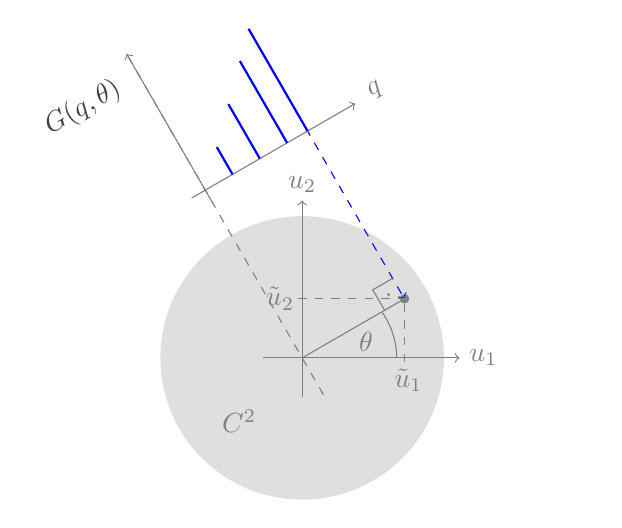
\begin{tikzpicture}[xshift=50]	
		\fill[nearly transparent, color=gray] (0,0) circle (1.8cm);
		\draw [gray] [->](-0.5,0) -- (2,0); % x-Achse
		\draw [gray] (2, 0) node [right] {$u_1$};
		
		\draw [gray] [->](0,-0.5) -- (0,2); % y-Achse
		\draw [gray] (0, 2.2) node {$u_2$};
		
		\fill[gray](1.3,0.75) circle [radius=0.06]; % ein Punkt		
		
		\draw [rotate=30, xshift=1.5cm, ->, dashed] [blue] (0,2.5) -- (0,0); % strahl		
		
		\draw [xshift=1.05cm, yshift=0.6cm, rotate=120, - ] [gray] (0,0) -- (0.3,0);
		\draw [xshift=0.89cm, yshift=0.86cm, rotate=30, - ] [gray] (0,0) -- (0.3,0);
		\draw [gray] (1.1, 0.8)  node {$.$};
		
		\draw [rotate=30] [gray] [-] (0,0) -- (1.5, 0);
		
		\draw [dashed] [gray] (1.3,-0.05) -- (1.3,0.75); % x-Projektion
		\draw [gray] (1.35,-0.28)  node {$\tilde{u}_1$};
		
		\draw [dashed] [gray] (-0.05,0.75) -- (1.3,0.75); % y-Projektion		
		\draw [gray] (-0.28,0.75)  node {$\tilde{u}_2$};
	
		\draw [rotate=30, xshift=0, yshift=70] [gray] [->] (-0.2,0) -- (2.2, 0);
		\draw [gray] (3.7, 0)  node [rotate=30, xshift=-20, yshift=123] {$q$};
		
		\draw [rotate=120, xshift=70 ] [gray] [->] (-0.2,0) -- (2, 0);	% g(s, \theta) line	
		\draw [rotate=120, xshift=70 ] [gray, dashed] [-] (-3,0) -- (2, 0);		
		\draw [darkgray] (-0.2, 0)  node [left, rotate=30, yshift=115] {$G(q, \theta)$};			
		
		\draw [gray] (1.2,0) arc [start angle=0, end angle=35, radius=1cm];
		\draw [gray] (0.6, 0.2) node [right] {$\theta$};
		
		\draw [gray] (-0.8, -0.8) node {$\mathbb{C}^2$};
		
		\foreach \x in {0, 0.4, 0.8, 1.2, 1.5}
		{
			\draw[rotate=30, xshift=0, yshift=70][blue, thick] (\x,\x) -- (\x,0); 
		}
	\end{tikzpicture}
	\caption{Eine Veranschaulichung des Fourier-Slice-Theorems. Links ist der Vorgang der Radon Transformation abgebildet, rechts seine Fouriertransformierte.}
	\label{fig:3.5}
\end{figure}

Jetzt haben wir genug Argumente gesammelt, um die gefilterte Rückprojektion herzuleiten. Dafür beginnen wir mit dem Punkt 1 des FST: wir bilden die Fouriertransformierte (Fußnote \ref{foot:14}) einer Projektion $p(s, \theta)$:
\begin{equation}
	\begin{split}
		P(q, \theta) & = \int \limits_{-1}^{1} p(s, \theta) e^{-2\pi i qs} \mbox{d}s \\
		&  \stackrel{(\ref{equa:1.10})}{=} \int \limits_{-1}^{1} \left( \int\limits_{-\gamma(s)}^{\gamma(s)} f(s\omega(\theta) + t\omega^{\perp}(\theta)) \mbox{d}t \right) e^{-2\pi i qs} \mbox{d}s \\
		& \stackrel{(\ref{equa:1.22})}{=} \int \limits_{\Omega} f(x) e^{-2\pi i q x^T\omega(\theta)}\mbox{d}x.	
	\end{split}
	\label{equa:3.14}
\end{equation}	
An dem Punkt 3 des FST ist nicht viel zu tun, deshalb geben wir hier direkt die Fouriertransformierte von $f$ an. Bei der Wahl der Koordinaten für $\mathcal{F}f$ und ihre Umrechnung stützen wir uns auf die rechte Seite der Abbildung \ref{fig:3.5}. Dann gilt 
\begin{equation}
	 F(q\cos(\theta), q\sin(\theta)) = \int \limits_{\Omega}^{} f(x)e^{-2\pi i qx^T\omega(\theta)} \mbox{d}x.
	\label{equa:3.15}
\end{equation}
Aus den Gleichungen (\ref{equa:3.14}) und (\ref{equa:3.15}) können wir festhalten, dass die Fouriertransformierten von $f$ und $p$ im folgenden Bezug zueinander stehen
\begin{equation}
	F(q\cos(\theta), q\sin(\theta)) =  P(q, \theta).
	\label{equa:3.16}
\end{equation}   
Das heißt (\ref{equa:3.16}) soll eine Koordinatentransformation zwischen $\mathcal{F}f$ und $\mathcal{F}p$ darstellen. Somit ist der Punkt 2 des FST auch erledigt.

Im zweiten Schritt invertieren wir die Gleichung (\ref{equa:3.15}) und führen eine Variablensubstitution\footnote{Für die Substitution von $\mbox{d}u_1\mbox{d}u_2$ berechnen wir die Jacobi-Determinante von $ |J(\left(\begin{array}{c} u_1 \\ u_2 \end{array}\right)) = \left| \left(\begin{pmatrix}{c} \cos(\theta) & \sin(\theta) \\ -q\sin(\theta) & q\cos(\theta) \end{pmatrix}\right)\right| = q$, somit erhalten wir $\mbox{d}u_1\mbox{d}u_2 = q\mbox{d}q\mbox{d}\theta$.} durch, sodass man zu der Gleichung  
\begin{equation}
	f(x) = \int \limits_{0}^{\pi} \int \limits_{-1}^{1}F(q\cos(\theta), q\sin(\theta))e^{2\pi i qx^T\omega(\theta)} q \ \mbox{d}q \ \mbox{d}\theta
	\label{equa:3.17}
\end{equation}
gelangt. Die Symmetriebetrachtungen, wie in \cite[S. 135]{Buzug04} und die Tatsache, dass man nur reelle Funktionen auf $\Omega$ betrachtet, führen zu folgendem Ausdruck
\begin{equation}
	\begin{split}
		f(x) & = \int \limits_{0}^{\pi} \int \limits_{-1}^{1}F(q\cos(\theta), q\sin(\theta))e^{2\pi i qx^T\omega(\theta)} |q| \ \mbox{d}q \ \mbox{d}\theta \\
		& \stackrel{(\ref{equa:3.16})}{=} \int \limits_{0}^{\pi} \left( \int \limits_{-1}^{1} \left( \ P(q, \theta)|q| \ \right) e^{2\pi i qx^T\omega(\theta)} \ \mbox{d}q \right) \mbox{d}\theta.
	\end{split}
	\label{equa:3.18}
\end{equation}

Mit der Gleichung (\ref{equa:3.18}) haben wir die gefilterte Rückprojektion erhalten. Es bleibt noch das Gefilterte darin zu entdecken. Beginnen wir mit der inneren Klammerung von (\ref{equa:3.18}). $P(q, \theta)$ ist die Fouriertransformierte $\mathcal{F}p$ von $p(s,\theta)$, die punktweise mit einer Betragsfunktion $b(q) = |q|$ multipliziert wird. Da wir jetzt $p(s, \theta)$ im Frequenzraum betrachten und die Funktion $b(q)$ über das gleiche Frequenzband, wie $P(q,\theta)$ läuft, werden durch punktweise Multiplikation kleinfrequente Anteile von $P(q,\theta)$ von $b(q)$ unterdrückt und die hochfrequente im Gegensatz sehr verstärkt. Dieses Vorgehen wird im Allgemeinen \textit{Hochpassfilterung} genannt. Die Funktion $b(q) = |q|$ bezeichnet man als Rampenfilter. Im Folgenden bezeichnen wir einen Filter mit $h_{\xi}(q)$ und wir schreiben $h_{b}(q) = b(q) = |q|$. Für die Filterung der Projektionen führen wir die Bezeichnung $P_{h_{\xi}}(q, \theta) = P(q, \theta)h_{\xi}(q)$ ein.

Nach dem die Filterung der Projektion durchgeführt wurde, wird diese mittels der inversen FT zurück in den Ortsrum der Projektionen überführt. Was durch das innere Integral von (\ref{equa:3.18}) dargestellt wird. Anschließend projiziert man die gefilterte Projektion in den Ortsraum von $f$ zurück, dies ist das äußere Integral von (\ref{equa:3.18}). 

Wir fassen die nötigen Schritte der gefilterten Rückprojektion zu einem Algorithmus zusammen
\begin{algorithm}
	\caption{Gefilterte Rückprojektion (Filtered Back Projection, FBP)}
	\begin{algorithmic}[1]	
		\State Berechne die FT von $(\mathcal{F}p)(s, \theta) = P(s, \theta)$.
		\State Führe die Fiterung $P_{h_{\xi}}(q, \theta) = P(q, \theta)h_{\xi}(q)$ durch.
		\State Berechne die inverse FT $(\mathcal{F}^{-1}P_{h_{\xi}})(q, \theta) = \tilde{p}(s,\theta)$.
		\State Projiziere $\tilde{p}(s,\theta)$ auf $\Omega$ zurück. 
	\end{algorithmic}
	\label{alg:3.1}
\end{algorithm}

In der Abbildung \ref{fig:3.6.b} ist das erste Ergebnis der gefilterten Rückprojektion, gefiltert mit einem Rampenfilter zu sehen. 

Wenn man das Sinogramm (Abb. \ref{fig:3.2.b}) betrachtet, so stellt man fest, dass das Sinogramm keine Störungen aufweist. Das würde eine perfekte Messung bedeuten. Dies ist aber bei den realen Messungen nie der Fall. Deshalb wollen wir uns die Rekonstruktion von gestörten Daten anschauen. Dafür soll das Phantom Bild (Abb. \ref{fig:3.2.a}) mit einem Salzstreuer-Effekt (Quelle: \MATLAB) beaufschlagt werden. Das soll die Homogenität einiger Pixelbereiche von der Abbildung \ref{fig:3.2.a} aufheben, was eine kleine Annäherung zur Realität widerspiegelt (Abb. \ref{fig:3.7.a}).  
\begin{figure}[!h]
	\begin{center}
		\subfloat[\label{fig:3.6.a}Das Rampenfilter.]{{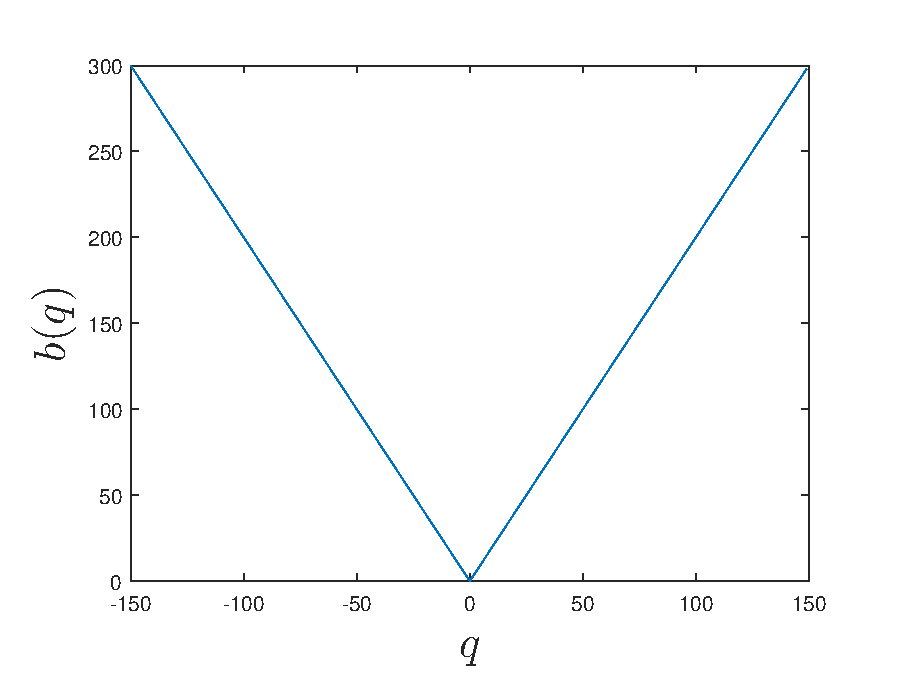
\includegraphics[width=0.5\textwidth]{rampFilter.eps} }}
		\subfloat[\label{fig:3.6.b}Eine mit Rampenfilter gefilterte Rückprojektion.]{{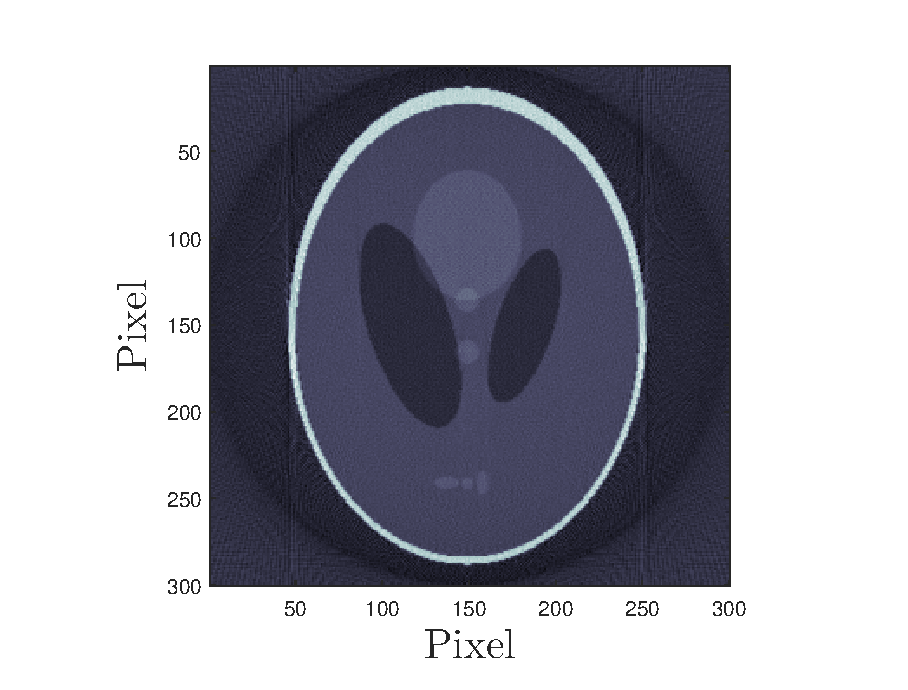
\includegraphics[width=0.5\textwidth]{rampFiltered.eps} }}
	\end{center}
	\caption{ Links (a) das Rampenfilter, konstruiert passend zu dem Sinogramm aus \ref{fig:3.2.b}. Das Frequenzband des Filters ist durch die isometrische Eigenschaften der FT gleich der Detektorbreite, also ist auch gleich der Tiefe des Sinogramms. Rechts (b) ist die gefilterte Rückprojektion von \ref{fig:3.2.b}, durchgeführt unter der Einwirkung des Rampenfilters aus (a).}
	\label{fig:3.6}
\end{figure} 

Die Radon Transformation von der Abbildung \ref{fig:3.7.a} ohne zusätzliche Störung würde nicht die Messfehler repräsentieren, höchstens Rundungsfehler, die bei der Integration entstehen, hier aber nicht wesentlich sind. Deshalb stören wir die Projektionsdaten zusätzlich mit dem Salzstreuer-Effekt (Abb. \ref{fig:3.7.b}).
\begin{figure}[!h]
	\begin{center}
		\subfloat[\label{fig:3.7.a}Ein verrauschtes Phantombild.]{{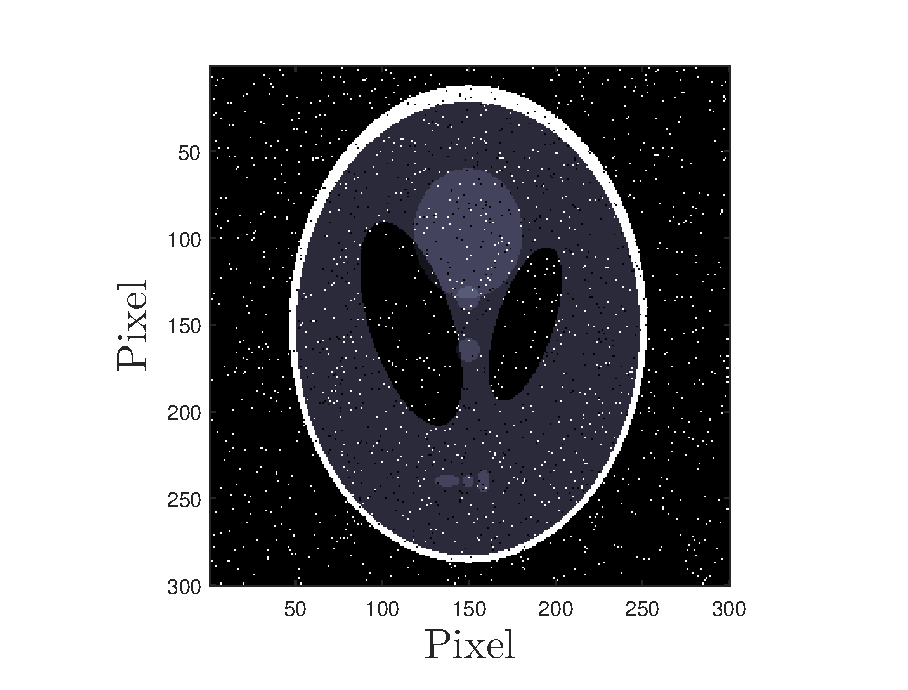
\includegraphics[width=0.5\textwidth]{noisedPhantom.eps} }}
		\subfloat[\label{fig:3.7.b}Die Radontransformierte von (a) und einem zusätzlichem Rauschen.]{{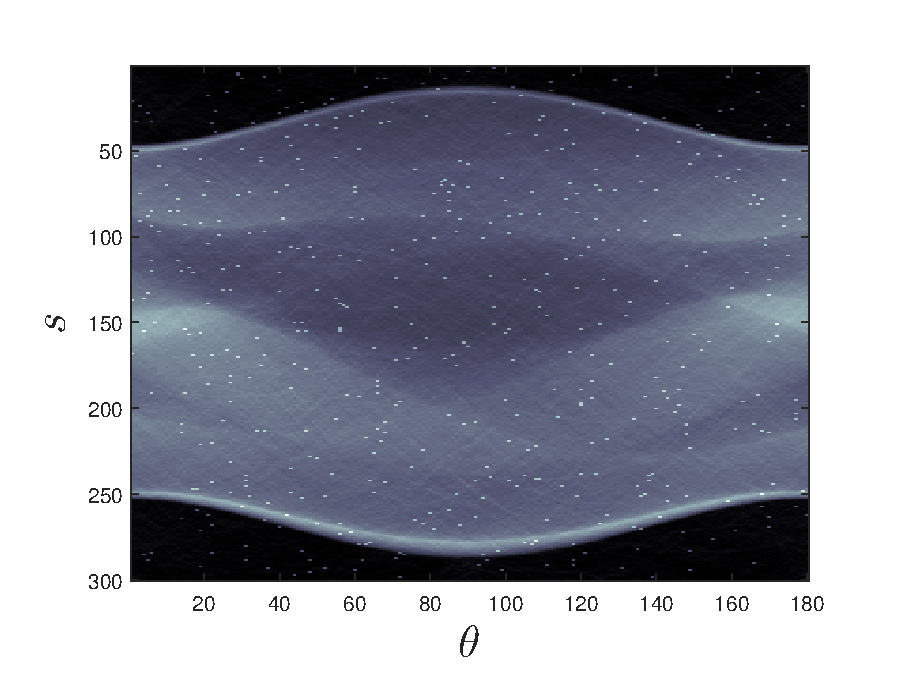
\includegraphics[width=0.5\textwidth]{rt_noised.eps} }}
	\end{center}
	\caption{ Links (a) ist ein Phantombild verrauscht mit einem Salzstreuer-Effekt (Quelle: \MATLAB) dargestellt. Rechts (b) ist Die Radontransformierte von (a) und zusätzlich mit einem Salzstreuer-Effekt verrauscht.}
	\label{fig:3.7}
\end{figure} 

Wir erinnern uns an die Ergebnisse des zweiten Kapitels. Insbesondere daran, dass der Operator $\mathcal{R}$ schlecht gestellt ist. Dazu sei die Gleichung (\ref{equa:2.3}) nochmal betrachtet
\[\mathcal{R}^{+} g  = \sum\limits_{j = 1}^{n} \sigma_j^{-1} \langle g, u_j \rangle_{L^2(Z)} v_j.\]
Wir wissen, dass $g$ die Projektionen in (\ref{equa:2.3}) darstellt. Sei nun $p_{\epsilon}$ unsere gestörte Projektion. Des Weiteren betrachten wir den Schritt 2,3 des Algorithmus \ref{alg:3.1} und schreiben ihn, wie folgt auf
\begin{eqnarray}
	\tilde{p}_{\epsilon} = \int \limits_{-1}^{1} P(q, \theta)h_{\xi}(q) e^{2\pi i qx^T\omega(\theta)} \ \mbox{d}q.
	\label{equa:3.19}
\end{eqnarray}
Wir wollen nun $\tilde{p}_{\epsilon}$ als eine Linearkombination oder auch als verallgemeinerte Fourierreihe angeben. Das tun wir direkt für den diskreten Fall unter Beachtung der Bemerkung \ref{bem:5}. Somit bekommen wir
\begin{equation}
	\tilde{p}_{\epsilon} \approx \sum \limits_{i = 1}^{n} c_ih_{\xi}(q_i)u_i, \ \ \mbox{mit} \  c_i = \langle \tilde{P}, u_i \rangle.
	\label{equa:3.20}
\end{equation} 
Diese Gleichung werden wir nicht beweisen, aber praktisch bedeutet das, wenn man $h_{\xi}(q) = 1$ setzt und es dem FBP Algorithmus übergibt, kommt genau die ungefilterte Projektion dabei raus.
\begin{figure}[!h]
	\centering
	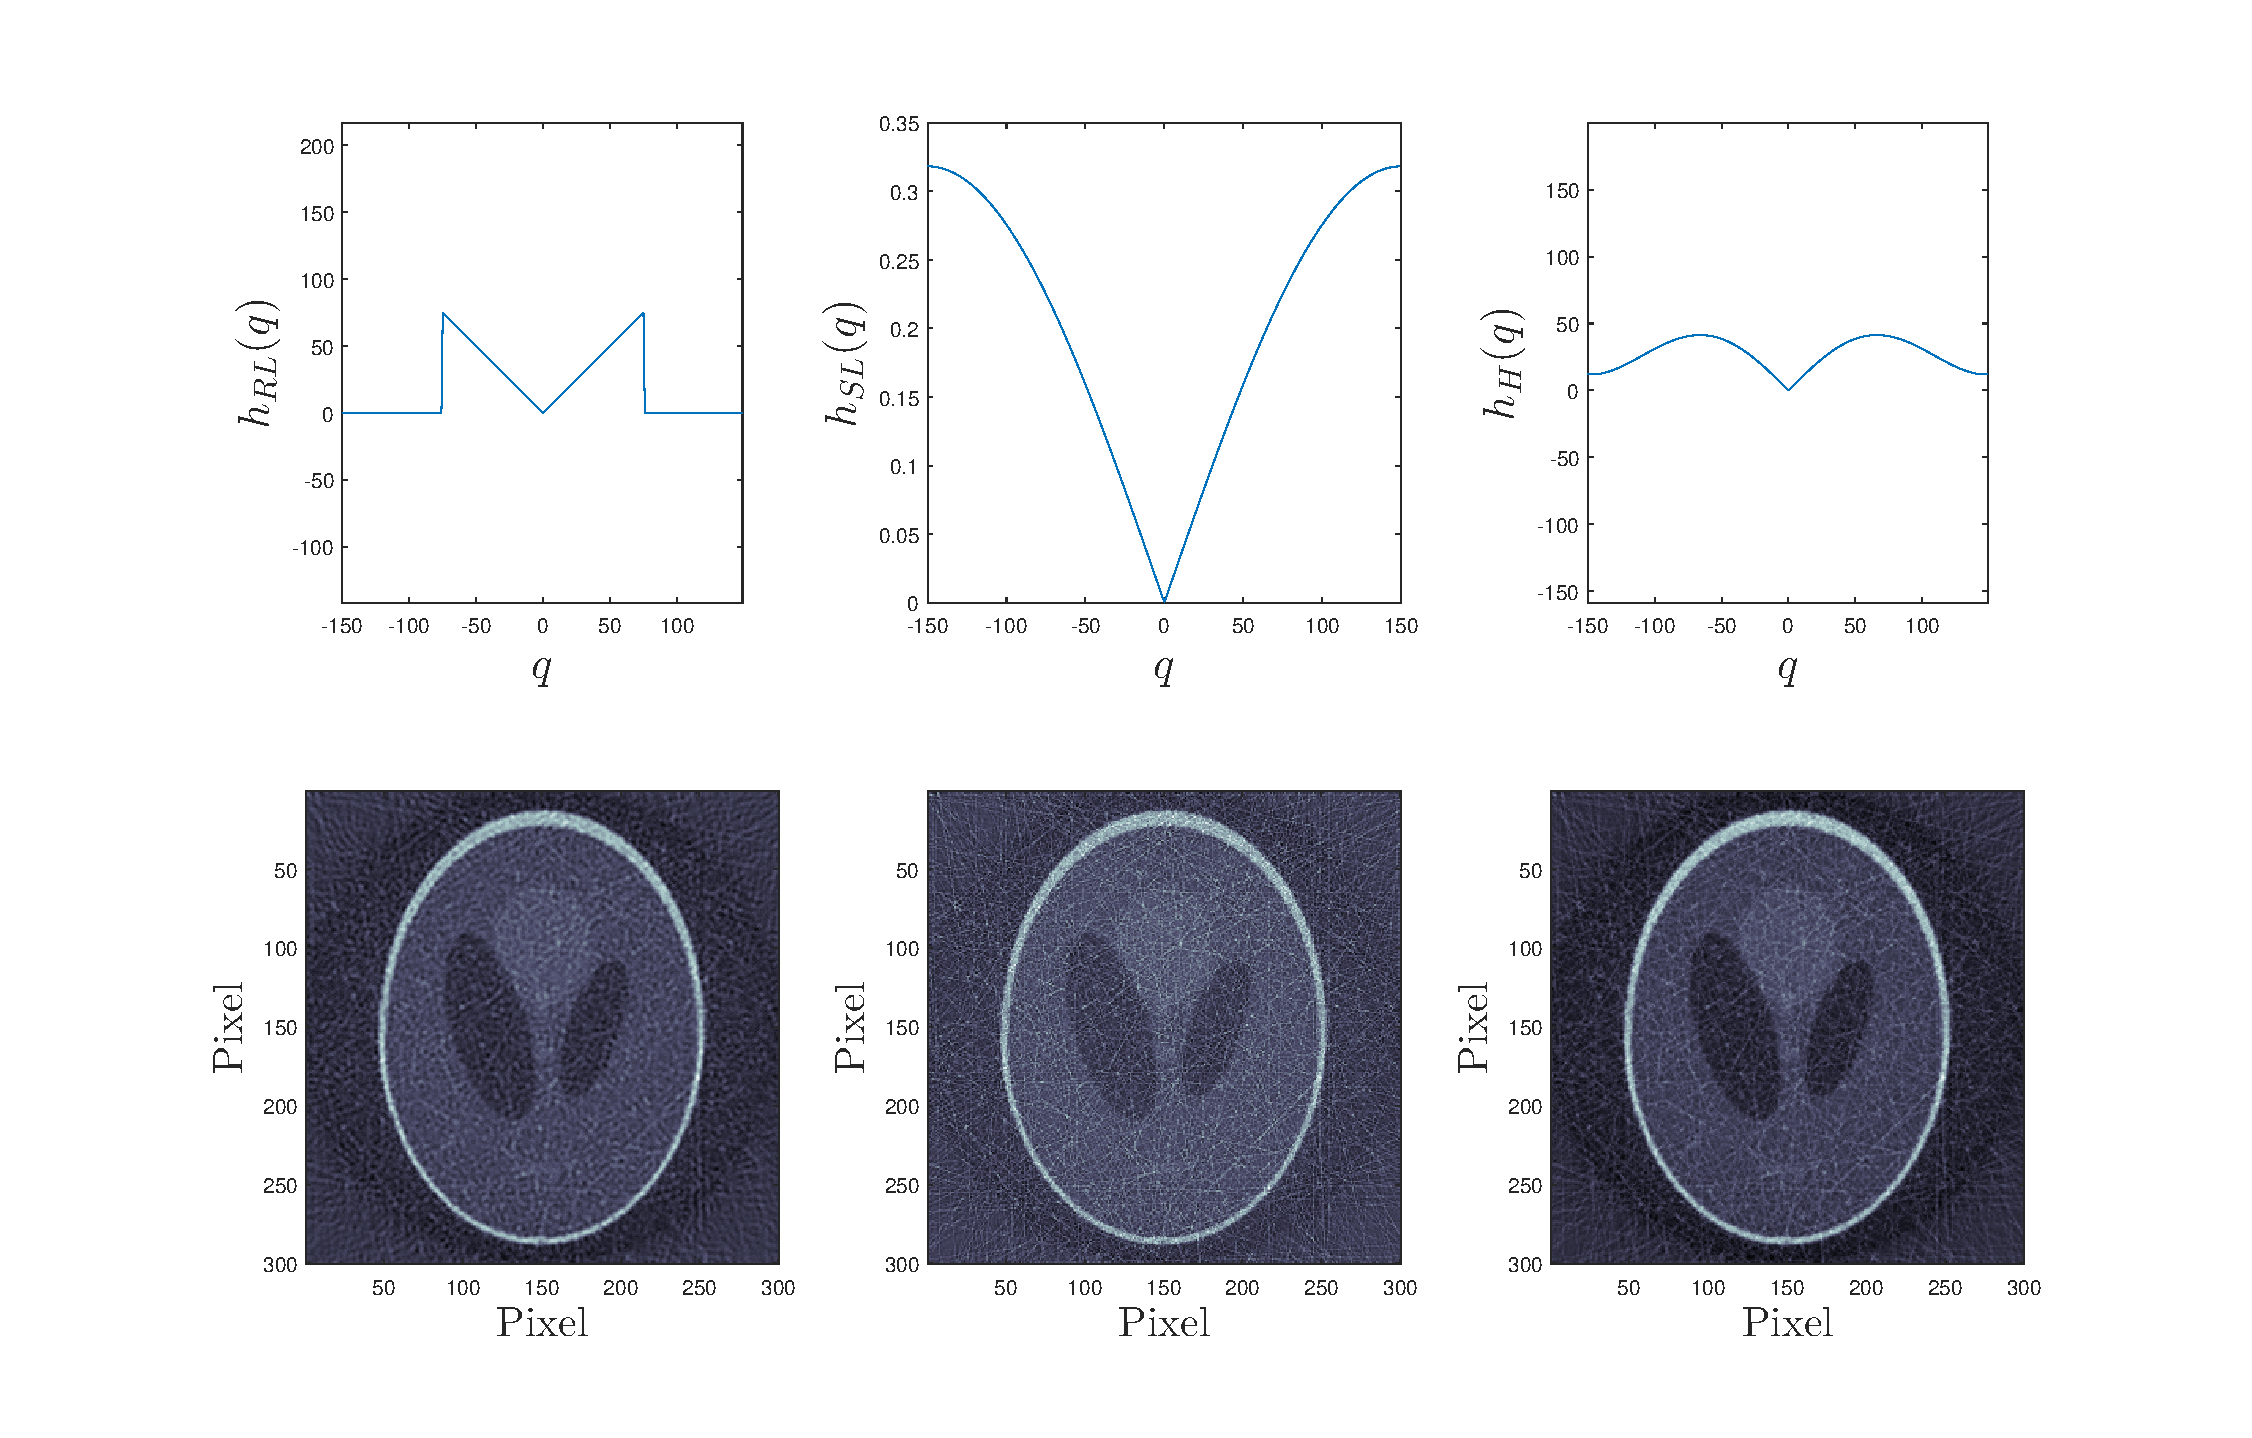
\includegraphics[width=1\textwidth]{diffFilter.eps}
	\caption{Eine Rekonstruktion aus den Daten \ref{fig:3.7.b} unter der Einwirkung von drei verschiedenen Filtern. Unten links ist die Filterung mit dem \textit{Ramachandran-Lakshminarayanan-Filter}, mittig mit dem \textit{Shepp-Logan-Filter} und rechts mit dem \textit{Hamming-Fiter} dargestellt.}  
	\label{fig:3.8}
\end{figure}

Nun setzen wir unsere gestört-gefilterte Projektion (\ref{equa:3.20}) in (\ref{equa:2.3}) ein und bekommen einen Ausdruck
\begin{equation}
	\begin{split}
		\mathcal{R}^{+} g & = \sum\limits_{j = 1}^{n} \sigma_j^{-1} \langle \left( \sum \limits_{i = 1}^{n} c_i h_{\xi}(q_i) u_i \right), u_j \rangle_{L^2(Z)} v_j \\
		& = \sum\limits_{j,i = 1}^{n} ( \sigma_j^{-1} h_{\xi}(q_j) ) c_i \delta_{ij} v_j = \sum\limits_{j = 1}^{n} ( \sigma_j^{-1} h_{\xi}(q_j) ) c_i v_j,
	\end{split}
	\label{equa:3.21}
\end{equation}
der uns prinzipiell keine neue Erkenntnis liefert, aber offensichtlich macht, wie die hochfrequenten Anteile bei der Rekonstruktion von dem Filter beeinflusst werden können. Das heißt, das Design des Filters kann die Rückprojektion in verschiedenen Frequenzbereichen dämpfen und somit ihre Oszillation bis zu einem gewissen Grade beschränken. Anders gesagt, wir beschleunigen somit die Konvergenz der Reihe (\ref{equa:3.21}) zu unseren Gunsten. 

In der Abbildung \ref{fig:3.8} sind drei Ergebnisse mit drei verschiedenen Filtern dargestellt. Zum Aufbau verschiedener Filterkerne sei man hier auf \cite[S. 191]{Buzug04} verwiesen. In der Abbildung \ref{fig:3.8} links unten, ist zu erkennen, dass ein \textit{Ramachandran-Lakshminarayanan-Filter} die hohen Frequenzen abschneidet, wodurch das Bild insgesamt an Kontrast verliert. Das untere Ergebnis in der Mitte zeigt, dass das \textit{Shepp-Logan-Filter} die mittleren Frequenzen anhebt, was die Helligkeit des Ergebnisses etwas erhöht. Das untere rechte Bild hat durch das \textit{Hamming-Fiter} volles Frequenzband erhalten, allerdings sind die hohen Frequenzen stark gedämpft worden.

Insgesamt existiert ein Dutzend Filter, die bei der CT-Bildrekonstruktion eingesetzt werden können. Dieses Vorgehen nennt man \textit{Regularisierung} des Rückprojektionsproblems mit Filtern.  

\section*{Algebraische Rekonstruktionsverfahren}
\label{cha:3.2}

Algebraische Verfahren basieren auf der Auffassung des Operators $\mathcal{R}$ als eine Matrix. Das hat zu Folge, dass man die Wirkung von $\mathcal{R}$ auf $f$ in Form eines linearen Gleichungssystems auffassen kann. Somit bekommen wir
\begin{equation}
	\mathcal{R}f = Af = p.
	\label{equa:3.22}
\end{equation}
\begin{Bemerkung}
	Für den Rest dieses Kapitels vereinbaren wir nur diskretisierte Systeme zu betrachten. 
	\label{bem:9}
\end{Bemerkung}
Mit der Bemerkung \ref{bem:9} und den vereinbarten Größen $f \in \R^m$ (\ref{equa:3.2}) und $p \in \R^n$ (\ref{equa:3.1}) ist $A$ eine endliche Matrix. $A$ wird \textit{Systemmatrix} des Abbildungssystems von $\mathcal{R}$ genannt. Wir werden zunächst die Entstehung und den Aufbau von $A$ etwas genauer anschauen. 

\subsubsection{Aufbau der Systemmatrix $A$ von $\mathcal{R}$}

Da $f \in \R^m$ und $p \in \R^n$ sind bedeutet es, dass $A \in \R^{n\times m}$ ist. Das heißt, die Zeilen von $A$ laufen über die Indizierung der Projektionen $p$, also die Zeile $j$ ist die $j$-te Projektion. Die Spalten von $A$ laufen über die Indizierung von $f$.

$f$ wird durch die Anzahl der Detektoren $k$ im Detektorband diskretisiert (Abb. \ref{fig:3.9}). Man kann also hypothetisch $f \in \R^{k\times k}$ annehmen. Lassen wir die Indizierung von $f$ Zeilenweise durchlaufen, so kommen wir genau auf $f \in \R^{k^2}$. Wobei nach (\ref{equa:3.2}) $k^2= m$ gilt.

Aus der Gleichung (\ref{equa:3.22}) können wir folgern, dass für $j$-te Projektion
\begin{equation}
	\sum \limits_{i = 1}^{m} a_{ji}f_i = p_j
	\label{equa:3:23}
\end{equation}
gelten muss. Beachtet man, dass nur die $f_j$ die vom Strahl getroffen worden sind zur Summe (\ref{equa:3:23}) beitragen, ergibt sich die Gleichung (\ref{equa:3.3}).
\begin{figure}[!h]
	\centering
	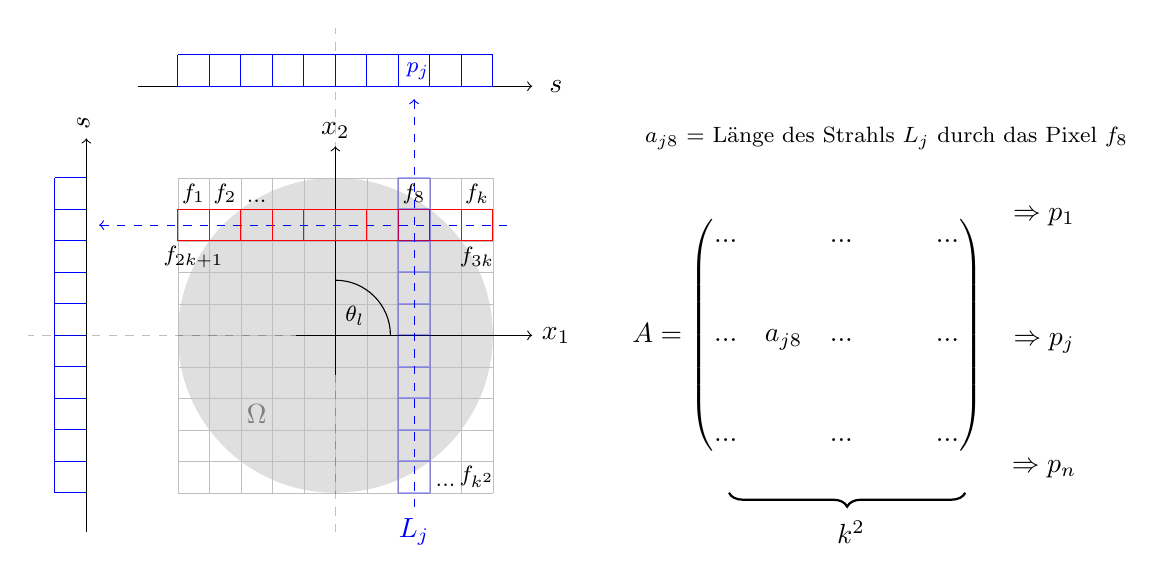
\begin{tikzpicture}
	\fill[nearly transparent, color=gray] (0,0) circle (2cm);
	\draw [gray] (-1, -1) node {$\Omega$};
	\draw [step=0.4,blue, thin, rotate=90, xshift=0, yshift=90] (-2,0) grid (2,0.4); % detector grid
	
	\draw [step=0.4, lightgray, very thin] (-2,-2) grid (2,2); % picture grid
	
	\draw [black] [->](-0.5,0) -- (2.5,0); % x-Achse
	\draw [black] (2.5, 0) node [right] {$x_1$};
	
	\draw [black] [->](0,-0.5) -- (0,2.4); % y-Achse
	\draw [black] (0, 2.6) node {$x_2$};
	
	\draw [rotate=90, xshift=0cm, <-, dashed] [blue] (1.4,3) -- (1.4,-2.2); % strahl
	%\draw [rotate=30, xshift=1.3cm ] [black] (0,-2.2) node {Röntgenstrahl};
	
	\draw [rotate=90, xshift=0, yshift=90] [black] [->] (-2.5,0) -- (2.5, 0);
	\draw [black] (2.8, 0)  node [rotate=90, xshift=2.7cm, yshift=6cm] {$s$};
	
	
	\draw [rotate=90, xshift=0cm, dashed] [nearly transparent, color=black] (0,-2.5) -- (0,3.9); % punktiert Mitte
	\draw [rotate=0, xshift=0cm, dashed] [nearly transparent, color=black] (0,-2.5) -- (0,3.9); % punktiert Mitte
	
	\draw [black] (0.7,0) arc [start angle=0, end angle=90, radius=0.7cm]; % angle \theta
	\draw [black] (0.25, 0.25) node {\footnotesize$\theta_l$};
	
	\draw [step=0.4, red, thin, rotate=90, xshift=1.2cm, yshift=0] (0,-2) grid (0.4,2);

	
	\draw [black] (0, 0)  node [rotate=0, xshift=1.4cm, yshift=-1.9cm] {\footnotesize$...$};
	\draw [black] (0, 0)  node [rotate=0, xshift=1.8cm, yshift=-1.8cm] {\footnotesize$f_{k^2}$};
		
	\draw [rotate=0, xshift=0, yshift=90] [black] [->] (-2.5,0) -- (2.5, 0);
	\draw [black] (2.8, 0)  node [rotate=0, xshift=0, yshift=90] {$s$};
	\draw [step=0.4,blue, thin, rotate=0, xshift=0, yshift=90] (-2,0) grid (2,0.4); % detector grid
	\draw [rotate=0, xshift=0cm, <-, dashed] [blue] (1,3) -- (1,-2.2); % strahl
	\draw [blue] (1,-2.5)  node {$L_j$};
	\draw [blue] (1.05,3.35)  node {\footnotesize$p_j$};
	\draw [step=0.4, blue, thick, opacity=0.3, rotate=0, xshift=0.8cm, yshift=0cm] (0,-2) grid (0.4,2);	
	
	\draw [black] (0, 0)  node [rotate=0, xshift=6cm, yshift=0cm] {$A = \begin{pmatrix}
		... & \ \ \ & ...& \ \ \ &  ... \\
		\ \ \\
		\ \ \\
		... & a_{j8} & ... & \ \ \ &  ... \\
		\ \ \\
		\ \ \\
		... & \ \ \ & ...& \ \ \ &  ... 
		\end{pmatrix}$};
	
	\draw [black] (0, 0)  node [rotate=0, xshift=9cm, yshift=1.5cm] {$\Rightarrow p_1$};
	\draw [black] (0, 0)  node [rotate=0, xshift=9cm, yshift=-0.1cm] {$\Rightarrow p_j$};
	\draw [black] (0, 0)  node [rotate=0, xshift=9cm, yshift=-1.7cm] {$\Rightarrow p_n$};	
	 
	\draw [thick,black,decorate,decoration={brace,amplitude=5pt}, rotate = 180, xshift=-6.5cm, yshift=2cm] (-1.5,0) -- (1.5,0);
	
	\draw [black] (0, 0)  node [rotate=0, xshift=-1.8cm, yshift=1.8cm] {\footnotesize$f_1$};
	\draw [black] (0, 0)  node [rotate=0, xshift=-1.4cm, yshift=1.8cm] {\footnotesize$f_2$};
	\draw [black] (0, 0)  node [rotate=0, xshift=-1cm, yshift=1.7cm] {\footnotesize$...$};
	\draw [black] (0, 0)  node [rotate=0, xshift=1cm, yshift=1.8cm] {\footnotesize$f_8$};
	\draw [black] (0, 0)  node [rotate=0, xshift=1.8cm, yshift=1.8cm] {\footnotesize$f_k$};
	\draw [black] (0, 0)  node [rotate=0, xshift=-1.8cm, yshift=1cm] {\footnotesize$f_{2k+1}$};
	\draw [black] (0, 0)  node [rotate=0, xshift=1.8cm, yshift=1cm] {\footnotesize$f_{3k}$};
	\draw [black, xshift=6.55cm, yshift=-2.5cm] (0, 0)  node {$k^2$};
	
	\draw [black, xshift=7cm, yshift=2.5cm] (0, 0)  node {\footnotesize$a_{j8}$ = Länge des Strahls $L_j$ durch das Pixel $f_8$};
	
	\end{tikzpicture}
	\caption{Eine Skizze zur Veranschaulichung des Aufbauprinzips der Abbildungsmatrix $A$ von $\mathcal{R}$.}
	\label{fig:3.9}
\end{figure}

Jetzt bleibt noch zu klären, wie das Systemmatrix $A$ initialisiert wird. In der Abbildung \ref{fig:3.9} sehen wir den Strahl $L_j$, der zu den Projektionen unter dem Winkel $\theta_1 = 0^{\circ}$ gehört. Der Strahl trifft unter anderen auch das Bildpixel $f_8$. Berechnet man die Länge des Strahls durch dieses Pixel, so kann man die errechnete Größe an der Stelle des Gewichts $a_{j8}$ in $A$ eintragen. Dementsprechend gilt es für alle betroffenen Pixel pro Strahl. 

Für jeden Winkel werden immer $k \in \N$ Projektionen erzeugt, so ergibt sich aus der Anzahl der Winkel $q \in \N$ die Anzahl der Projektionen $n = kq$, was dem Ausdruck (\ref{equa:3.1}) entspricht.   

Zu bemerken ist noch, dass die Matrix $A$ eine \textit{dünnbesetzte} Matrix ist. Mann kann leicht einsehen, dass auf der Diagonalen von $f$ maximal $\lfloor\sqrt{2}\rfloor k$ Pixel liegen. Wenn der Strahl etwas neben der Diagonalen parallel verläuft, trifft er höchstens $2\lfloor\sqrt{2}\rfloor k - 1$ Pixel von $f$; dies ist auch die maximale Anzahl der Einträge von $A$ in einer Zeile.

\begin{Bemerkung}
	Die Längen des Strahls pro Pixel zu berechnen, ist nicht die einzige Möglichkeit $A$ zu modellieren. Die Gewichte $a_{ji}$ können auch als Verhältnis der Fläche des Strahls zu der Pixelfläche aufgestellt werden. Das modelliert zwar das Abbildungssystem von $\mathcal{R}$ besser, ist aber viel rechenaufwendiger, als die hier betrachtete Vorgehensweise \cite[S. 141]{Zeng09}.
\end{Bemerkung}
Die Implementierung der Funktion zur Erstellung der Systemmatrix ist in \ref{cha:A.4} kommentiert und ist auf der beigelegten CD-ROM einzusehen.\\\\

Nachdem die Konstruktion der Systemmatrix etwas erhellt wurde, wollen wir zu der Diskussion der darauf aufbauenden Rekonstruktionsverfahren übergehen. Die sogenannten \textit{algebraische Rekonstruktionstechniken} (eng. \textit{algebraic reconstruction technique, ART}) beruhen auf der Kenntnis von $A$. Als erstes würde man wahrscheinlich auf die Idee kommen, die Gleichung $Af = p$ zu invertieren. Nun in der Regel ist $A$ sehr groß und hat keine einfache Struktur, sodass keine schnelle Inversion gefunden werden kann und wenn, dann ist es sehr zeit- und speicherintensiv (vergl. \cite[S. 157]{Burg91}). Zudem kann es vorkommen, dass $m > n$ ist, was heißen würde, dass das System unterbesetzt ist und dadurch keine eindeutige oder gar keine Lösung haben kann. Deshalb sucht man nach anderen Techniken $f$ zu rekonstruieren.

\subsection*{Iterative Rekonstruktion nach Kaczmarz}
\label{cha:3.2.1}

In diesem Abschnitt wollen wir ein iteratives Verfahren zur Lösung des Gleichungssystems (\ref{equa:3.22}) nach Kaczmarz\footnote{Stefan Kaczmarz (1895-1939) polnischer Mathematiker.} anschauen. Das Verfahren kann folgendermaßen hergeleitet werden. Dafür betrachten wir (\ref{equa:3.22}) in expandierter Form
\begin{equation}
	\begin{split}
		a_{11}f_1 + \ \ \dots \ \ + a_{1m}f_m & = p_1 \\
		& \ \ \vdots\\
		a_{j1}f_1 + \ \ \dots \ \ + a_{jm}f_m & = p_j \\
	    & \ \ \vdots\\
		a_{n1}f_1 + \ \ \dots \ \ + a_{nm}f_m & = p_n.
	\end{split}
	\label{equa:3.24}
\end{equation}
So stellt jede der obigen Gleichungen eine Hyperebene $H_j = \{ f \in \R^m | \langle a_j , f \rangle = p_j, \ j \in [1,n], n \in \N  \}$ dar. Hier ist $a_j$ die $j$-te Zeile von $A$. Damit liegt die Lösung von (\ref{equa:3.24}) genau in dem Schnittpunkt aller Ebenen, was in diesem Falle $f \in \R^m$ bedeuten würde. 

Zum Suchen von $f$ bietet sich die Methode der Lotprojektion an. Dafür wählt man einen beliebigen Punkt $f_0$ und projiziert einen Lot von $f$ aus auf eine beliebige Hyperebene $H_j$. Der Schnittpunkt des Lots mit $H_j$ ist dann $f_1$. Von $f_1$ aus projiziert man auf die nächste Hyperebene, so initialisiert man $f_2$ und so weiter, bis man an dem Schnittpunkt $f$ angekommen ist (Abb. \ref{fig:3.10}). 

Dieses Vorgehen beschreibt genau die Arbeitsweise des Algorithmus, also das Kaczmarz-Verfahren. Man unterscheidet zwischen dem vorwärts projektiven Verfahren und dem randomisierten. Der Unterschied besteht nur darin, dass bei dem ersten Verfahren die Projektionen auf die Ebenen der Reihe nach berechnet werden und in dem zweiten Verfahren werden die Ebenen zufällig ausgewählt.
\begin{figure}[H]
	\centering
	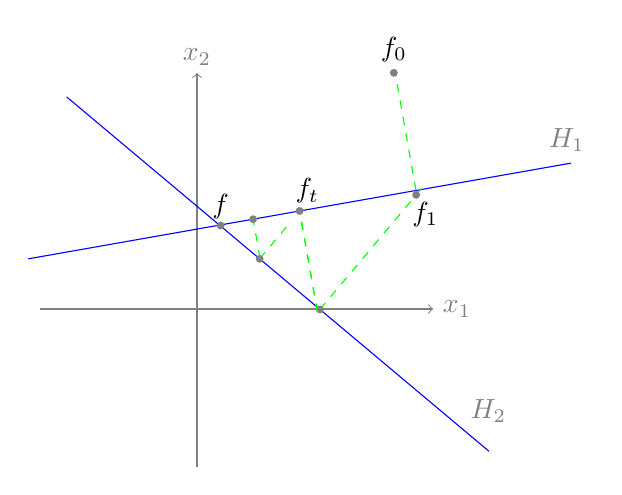
\begin{tikzpicture}
	
	\draw [gray] [->](-2,0) -- (3,0); % x-Achse
	\draw [gray] (3, 0) node [right] {$x_1$};
	
	\draw [gray] [->](0,-2) -- (0,3); % y-Achse
	\draw [gray] (0, 3.2) node {$x_2$};
	
	\draw [rotate=-40, xshift=1cm, yshift=1cm] [blue] (3,0) -- (-4,0); % blue ray	
	\draw [gray, xshift=3.7cm, yshift=-1.3cm] (0,0) node {$H_2$};
	
	\draw [rotate=10, xshift=1cm, yshift=1cm] [blue] (4,0) -- (-3,0); % blue ray
	\draw [gray, rotate=10, xshift=5cm, yshift=1.3cm] (0,0) node {$H_1$};
	
	\draw [rotate=100, xshift=1cm, yshift=-3cm, dashed] [green] (0,0) -- (1.5,0); % green from strat
	\fill[color=gray, xshift=1cm, yshift=3cm] (1.5,0) circle (0.05cm); % f point
	\draw [color=black, xshift=1cm, yshift=3cm] (1.5,0.3) node {$f_0$};
	
	\draw [rotate=50, xshift=1cm, yshift=-1.2cm, dashed] [green] (0,0) -- (2,0); % green from strat
	\fill[color=gray,rotate=50, xshift=1.4cm, yshift=-1.2cm] (1.5,0) circle (0.05cm); % f 1 point
	\draw [color=black,xshift=1.4cm, yshift=1.2cm] (1.5,0) node {$f_1$};
		
	\draw [rotate=100, xshift=-0.3cm, yshift=-1.5cm, dashed] [green] (0,0) -- (1.3,0); % green from strat	
	\fill[color=gray,rotate=50, xshift=1cm, yshift=-1.2cm] (0,0) circle (0.05cm); % f 2 point
	%\draw [color=black, xshift=1.45cm, yshift=-0.2cm] (0,0) node {$f_2$};
		
	\draw [rotate=100, xshift=-0.3cm, yshift=-1.5cm, dashed] [green] (0,0) -- (1.3,0); % green from strat	
	\fill[color=gray,rotate=100, xshift=-0.3cm, yshift=-1.5cm] (1.3,0) circle (0.05cm); % f 3 point
	\draw [color=black, xshift=0.1cm, yshift=1.5cm] (1.3,0) node {$f_t$};
	
	\draw [rotate=50, xshift=0.3cm, yshift=-0.2cm, dashed] [green] (0.7,0) -- (1.3,0); % green from strat		
	\fill[color=gray, rotate=50, xshift=0.3cm, yshift=-0.2cm] (0.7,0) circle (0.05cm); % f 4 point
	%\draw [color=black, xshift=0.1cm, yshift=0.3cm] (0.7,0) node {$f_4$};
	
	\draw [rotate=100, xshift=-0.2cm, yshift=-0.9cm, dashed] [green] (0.7,0) -- (1.3,0); % green from strat	
	\fill[color=gray, rotate=100, xshift=-0.2cm, yshift=-0.9cm] (1.2,0) circle (0.05cm); % f point
	
	\fill[color=gray, xshift=0.3cm, yshift=1.06cm] (0,0) circle (0.05cm); % f point
	\draw [color=black, xshift=0.3cm, yshift=1.3cm] (0,0) node {$f$};	
	
	\end{tikzpicture}
	\caption{Eine Veranschaulichung der Arbeitweise des Kaczmarz-Verfahrens in $\R^2$.}
	\label{fig:3.10}
\end{figure}

\begin{Bemerkung}
	Die Abbildung \ref{fig:3.10} zeigt ein Fall, wo die Lösung immer gefunden werden kann, denn der Schnittpunkt zweier Geraden ist immer exakt bestimmbar. Schon ab $\R^n$ für $n \geq 2$ ändert sich die Situation in den realen Fällen drastisch. Der Grund dafür ist, dass man ein mit Rauschen behaftetes System $Af \approx p + \epsilon$ hat. Somit ist jede Hyperebene $H_j$ um ein $\epsilon_j, \ j \in [1, n], \ n \in \N$ von dem Schnittpunkt verschoben. Das heißt, dass die Lösung $\tilde{f} \approx f$ in einem kleinem Toleranzvolumen $\prod \limits_{j=1}^{n}\epsilon_j$ liegt und daher nur annähernd angebbar ist.
	\label{be.:11}
\end{Bemerkung}

In \cite{Neufeld15} wird gezeigt, dass das randomisierte Verfahren eine schnellere Konvergenz nachweist. Aus diesem Grund werden wir dieses Vorgehen in Betracht ziehen. 
\begin{Definition}[Randomisierter Kaczmarz-Algorithmus]
	Sei $Af = p$ ein konsistentes, lineares Gleichungssystem. Sei $f_0 \in \R^m$ ein beliebiger Startwert. Für $t = 0, 1, 2, ...$ ist der Randomisierte Kaczmarz-Algorithmus definiert als
	\begin{equation}
			f_{t+1} = f_t + \frac{p_j - \langle a_j, f_t \rangle}{\parallel a_j \parallel_{2}^{2}}a_j,
			\label{equa:3.25}
	\end{equation}
	wobei $a_j$ die $j$-te Zeile von $A$ ist und $p_j$ die dazugehörige Projektion. $j$ wird zufällig ausgewählt.
	\label{def:5}	
\end{Definition} 
Wir wollen nun (\ref{equa:3.25}) etwas besser verstehen. Dafür formen wir diese Gleichung etwas um und bekommen

\[f_{t+1} = f_t + \left( \frac{p_j}{\parallel a_j \parallel_{2}} - \langle \frac{a_j}{\parallel a_j \parallel_{2}}, f_t \rangle \right) \frac{a_j}{\parallel a_j \parallel_{2}}.\]

Der eingeklammerte Teil der Gleichung stellt den Abstand von $f_t$ zu der $j$-ten Hyperebene $H_j$ in der Hesseschen Normalform Darstellung dar. Die Multiplikation mit $\frac{a_j}{\parallel a_j \parallel_{2}}$ liefert die Orthogonalität zu der $H_j$. Somit haben wir die oben beschriebene Lotprojektion, oder auch orthogonale Projektion auf $H_j$ genannt. 

Nun wollen wir uns von der Qualität des Verfahrens überzeugen, dessen genaue Implementierung in \ref{cha:A.5} (insbesondere die Abbruchbedingung (\ref{equa:A.1}) des Verfahrens) erläutert ist. Dazu sei die Abbildung \ref{fig:3.11} betrachtet. Die Ergebnisse in der Abbildung \ref{fig:3.11} wurden unter den gleichen Bedingungen, wie für die gefilterte Rückprojektion in den Abbildungen \ref{fig:3.6} für ungestörte und \ref{fig:3.8} (mittig) für gestörte Daten erzeugt. 

Man erkennt, dass die Ergebnisse der iterativen Rekonstruktion optisch gleichviel (oder sogar mehr) Informationsgehalt bieten, wie die der gefilterten Rückprojektion.
\begin{figure}[!h]
	\begin{center}
		\subfloat[\label{fig:3.11.a}Iterative Rekonstruktion aus nicht verrauschten Daten von \ref{fig:3.2.b}.]{{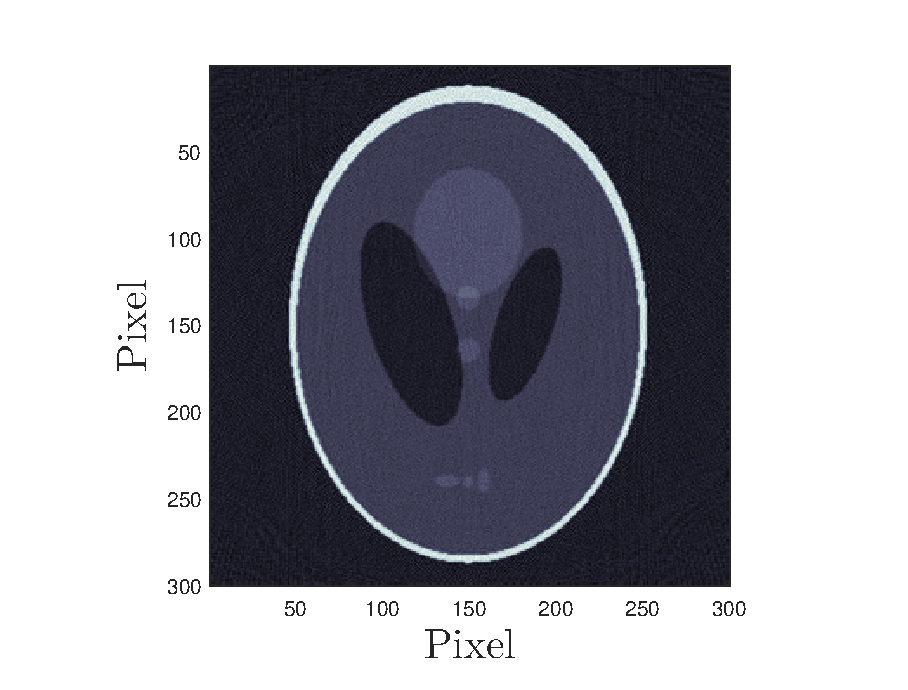
\includegraphics[width=0.5\textwidth]{iter.eps} }}
		\subfloat[\label{fig:3.11.b}Iterative Rekonstruktion aus verrauschten Daten von \ref{fig:3.7.b}]{{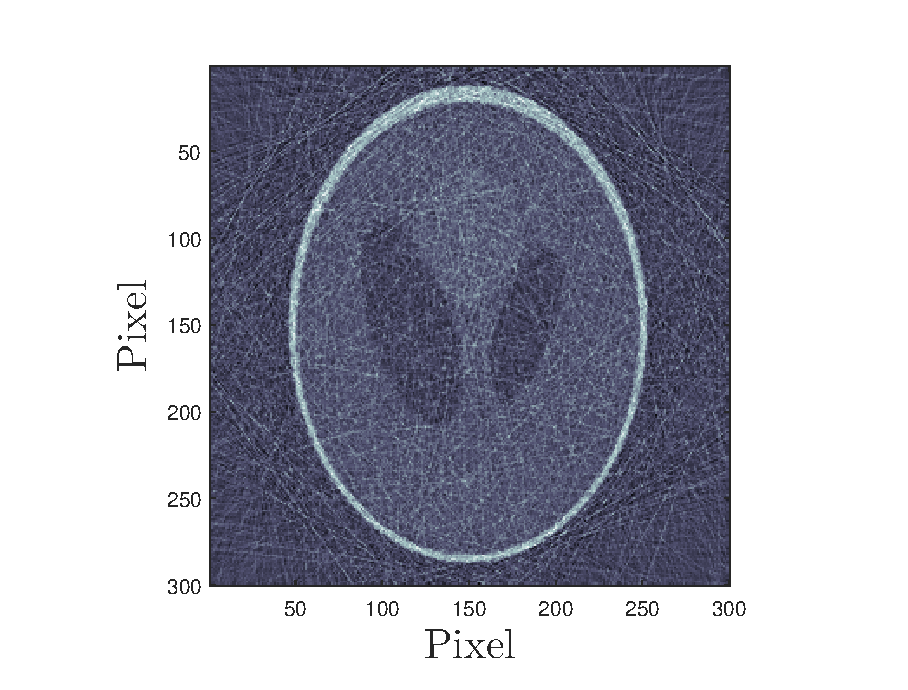
\includegraphics[width=0.5\textwidth]{iterNoised.eps} }}
	\end{center}
	\caption{Randomisierte iterative Rekonstruktionen (a) nicht verrauscht, (b) verrauscht. Die Projektionen in Beiden Fällen wurden für alle Winkel $\theta$ von $1^{\circ}$ bis $180^{\circ}$ mit der Schrittweite von $1^{\circ}$ berechnet. Detektorbreite ist $k=300$.}
	\label{fig:3.11}
\end{figure}

Jetzt wollen wir experimentell an einem Beispiel nachweisen, dass das randomisierte Verfahren in der Tat schneller konvergiert als das vorwärts projektive. Für unsere Testzwecke wählen wir ein Phantombild mit der Größe $50\times50$ Pixel (\MATLAB, \verb|phantom(50)|). Die kleine Größe des Phantombildes soll die Größe der Systemmatrix in annehmbaren Rahmen halten, da sonst zu große Matrizen entstehen, die sehr lange Rechenzeiten brauchen werden. Schließlich wollen wir nur die Konvergenz des Verfahrens untersuchen.
\begin{figure}[!h]
	\begin{center}
		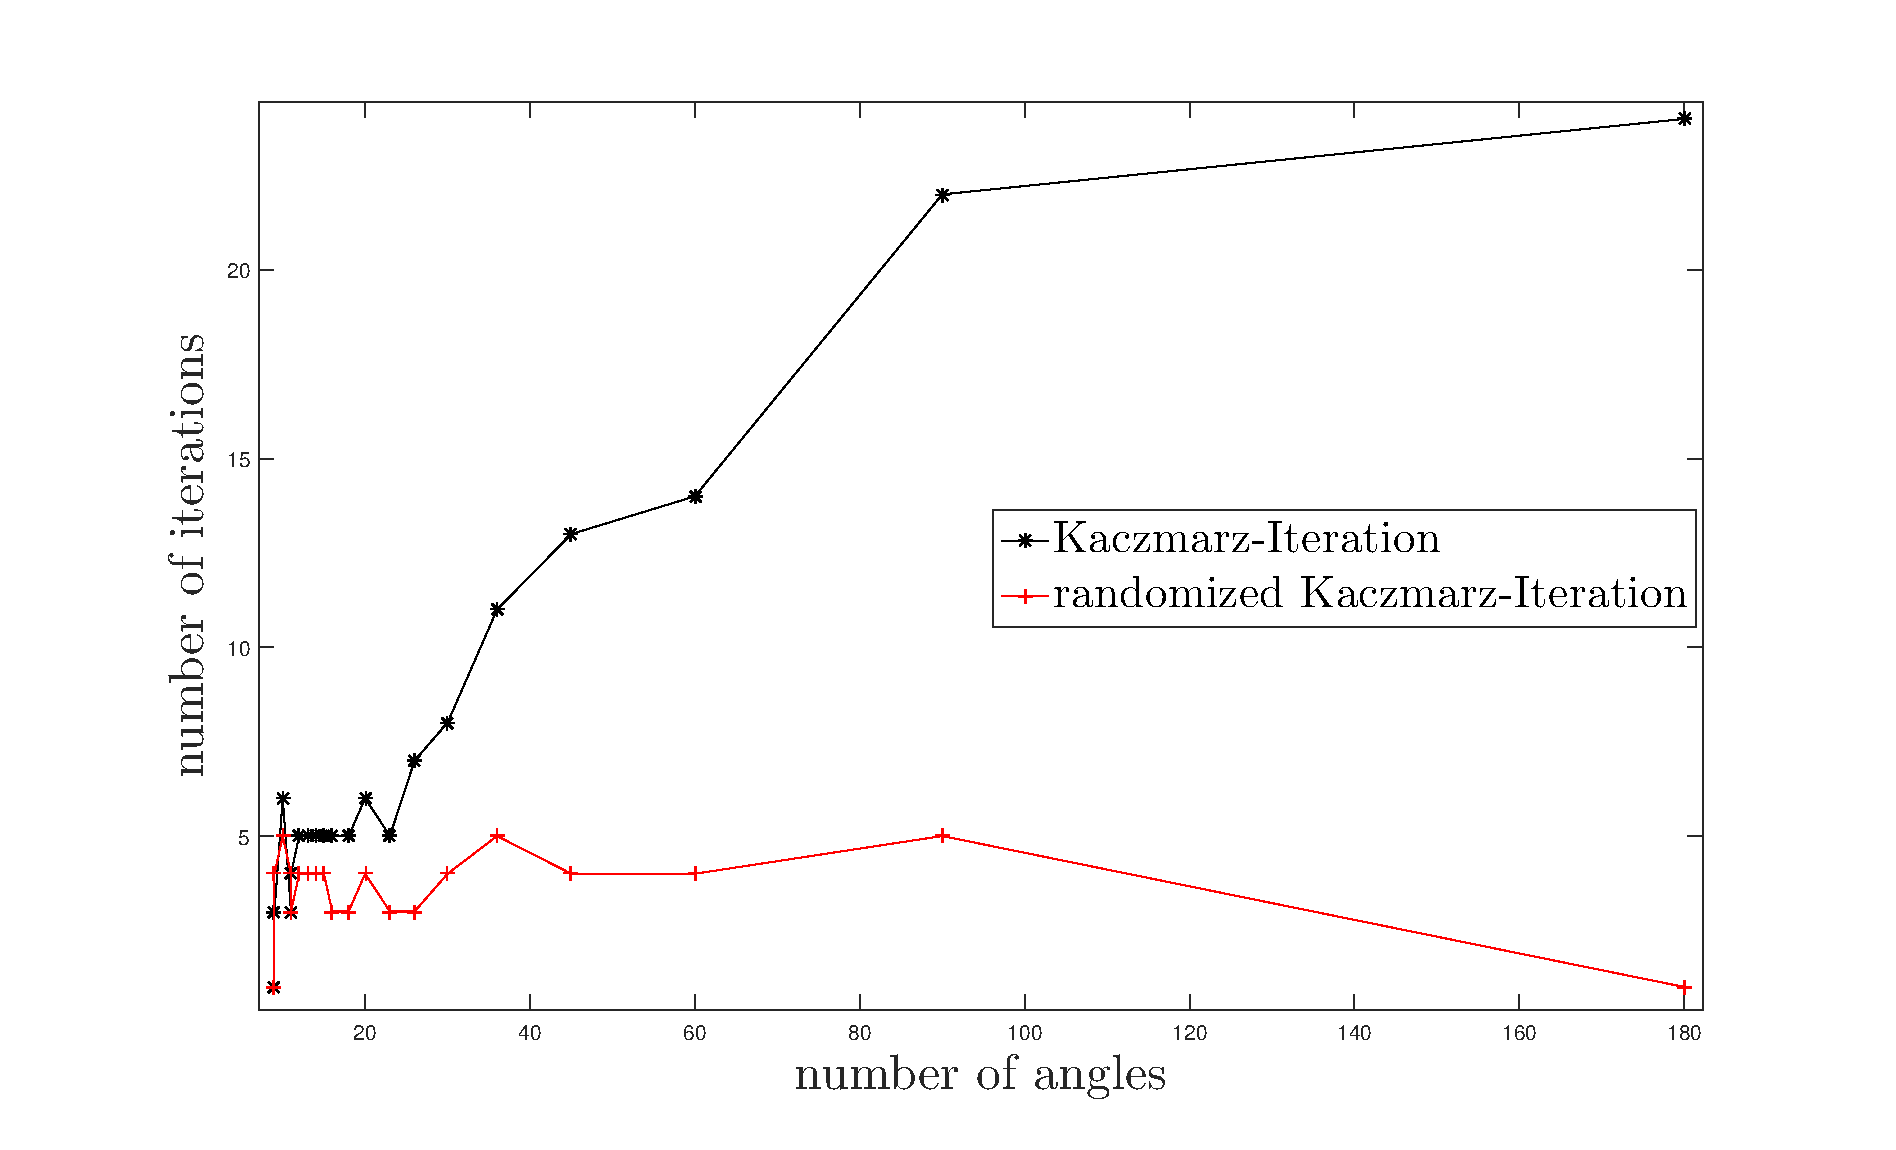
\includegraphics[width=\textwidth]{iterVSforward.eps}
	\end{center}
	\caption{Ein Vergleich des randomisierten und vorwärts projektiven Kaczmarz-Verfahrens. Der Test wurde für die Rekonstruktion eines $50 \times 50$ Pixel großen Bildes durchgeführt. In jedem Testschritt wurde die Winkelanzahl erhöht, sodass die Systemmatrix immer größer wurde.}
	\label{fig:3.12}
\end{figure}

In der Abbildung \ref{fig:3.12} ist das Ergebnis des Tests aus verrauschten (Salzstreuer-Effekt) Daten zu sehen. Dabei wurde die Systemmatrix in jedem Testschritt vergrößert, indem sich die Winkelanzahl und somit die Projektionsanzahl erhöhten. Der erste Testschritt wurde mit einer Winkelschrittweite von 20°, also für $q = 9$ Winkelpositionen durchgeführt. Die Detektorbreite wurde mit $k = 50$ initialisiert, was insgesamt für $A \in \R^{450\times2500}$ im erstem Testschritt ergeben hat. Der Test wurde bis $q = 180^{\circ}$ mit der Winkelschrittweite von 1°, das heißt bis $A \in \R^{9000 \times 2500}$ durchgeführt.

Die Abbruchbedingung musste für jeden Testschritt angepasst werden, da die Größe von $A$ schrittweise erhöht wurde und damit auch die Fehleranfälligkeit des Verfahrens. Aus (\ref{equa:A.1}) folgt $\delta = \alpha\epsilon$, wo $\epsilon = ||p - \tilde{p}||_2$ der Norm des Fehlers. $\alpha$ wurde als Verhältnis der Zeilenanzahl von $A$ im jetzt-Schritt zu davor-Schritt multipliziert mit dem Verhältnis der Winkelanzahl im jetzt-Schritt zu davor-Schritt aufgefasst. Da die Abbruchbedingung für beide Verfahren gleich war, kann man den Test als fair annehmen.

\subsection*{Rekonstruktion durch SWZ}
\label{cha:3.2.2}

Das letzte Verfahren, das wir uns anschauen werden beruht auf der Singulärwertzerlegung einer Matrix. Bekanntlich besitzt jede Matrix $A \in \R^{n\times}$ (wir beschränken uns hier auf reelle Matrizen) mindestens eine SWZ, sodass $A = U\Sigma V^{*}$ geschrieben werden kann. $U \in \R^{m\times m}$ ist die \textit{unitäre} Matrix des Bildes von $A$, $\Sigma \in \R^{m \times n}$ beinhaltet die Singulärwerte von $A$ auf der Diagonale sonst überall Null und $V^*$ ist die adjungierte der unitären Matrix des Kerns von $A$. Somit lässt sich die Gleichung (\ref{equa:3.22}) in der Form 
\begin{equation}
	Af = (U\Sigma V^*)f = p
	\label{equa:3.26}
\end{equation}
schreiben. Aus der Definition der unitären Matrizen folgt $U^{-1} = U^*$ und $(V^*)^{-1} = (V^*)^* = V$. Da $\Sigma$ eine Diagonalmatrix mit Singulärwerten größer Null ist, kann $\Sigma$ wie folgt invertiert werden
\begin{equation}
	\Sigma^+ = \left\{ \begin{matrix} \frac{1}{\sigma_{ji}} & : & \mbox{falls} \ j = i \\ 0 & : & \mbox{sonst} \end{matrix}\right. .
	\label{equa:3.27}
\end{equation}
Somit kann die Gleichung (\ref{equa:3.26}) invertiert werden, also
\begin{equation}
	f = (V\Sigma^+ U^*)p.
	\label{equa:3.28}
\end{equation}
Schreibt man die Gleichung \ref{equa:3.28} in expandierter Form auf
\begin{equation}
	f_i = \sum\limits_{i = 1}^{m}[\Sigma^+]_{ii} \langle p, u_i \rangle v_i,
	\label{equa:3.29}
\end{equation}
was mit $[\Sigma^+]_{ii} = \sigma^{-1}_{i}$ genau (\ref{equa:2.3}) entspricht. 

Mit den Ergebnissen aus dem Kapitel \ref{cha:2} wissen wir, dass bereits kleine Fehler in dem Messprozess stark oszillierend auf die Lösung (\ref{equa:3.29}) wirken können. Somit bedarf es einer Regularisierung in der Rekonstruktion. Wir werden die \textit{Tikhonov\footnote{Andrei Nikolajewitsch Tichonow (1906-1993) russischer Mathematiker.}-Regularisierung} benutzen, die wie folgt aufgeschrieben werden kann:
\begin{equation}
	d_i = \frac{\sigma_i}{\lambda^2 + \sigma_i^2}.
	\label{equa:3.30}
\end{equation}
Man erkennt, dass die Regularisierung für $\lambda = 0$ keine Wirkung ergibt. Ist $\lambda \geq 0$ so wirkt die Regularisierung dämpfend auf $\sigma_i$ und verhindert bei großen Werten die Oszillation der Lösung. Wir ersetzen die Elemente auf der Diagonale von $\Sigma^+$ mit (\ref{equa:3.30}) und benennen die Matrix mit $D$
\begin{equation}
	\tilde{f}_i = \sum\limits_{i = 1}^{m}[D]_{ii} \langle p, u_i \rangle v_i.
	\label{equa:3.31}
\end{equation} 

Wir wollen unsere Untersuchungen an dem Phantom-Beispiel (\verb|phantom(50)|) weiterführen. Wie in dem vorherigen Abschnitt werden die Daten mit dem Salzstreuer-Effekt beaufschlagt, sowie anschließend auch die Messdaten. Dabei wurden die Projektionen für 50 Winkel mit der Schrittweite von 3.6° aufgenommen. Folglich bekommt man eine Systemmatrix $A \in \R^{2500 \times 2500}$.

Nun wollen wir die Wirkung der Regularisierung (\ref{equa:3.31}) auf die Reihe (\ref{equa:2.4}) aus dem Satz \ref{satz:3} an unserem Beispiel verifizieren. Zunächst lassen wir das Verfahren (\ref{cha:A.6}) für verschiedene $\lambda$ das Phantombild rekonstruieren und tragen den entstandenen Rekonstruktionsfehler $||A\tilde{f} - p ||_2$ gegen $\lambda$ in einem Diagramm auf. Das Ergebnis ist in der Abbildung \ref{fig:3.13.a} zu sehen. Zu erkennen ist, dass der minimale Fehler etwa bei $\lambda_{min} = 5.5$ liegt (Abb. \ref{fig:3.13.a}). Anschließend lassen wir die Reihe (\ref{equa:2.4}) für zwei Parameter laufen, also $\lambda = 0$ und $\lambda_{min} = 5.5$. In der Abbildung \ref{fig:3.13.b} ist deutlich zu erkennen, dass die Reihe mit regularisierten Singulärwerten schneller konvergiert als die ohne Regularisierung.
\begin{figure}[!h]
	\begin{center}
		\subfloat[\label{fig:3.13.a}Der Fehler bei der Lösung durch SWZ in abhängigkeit von dem Regularisierungsparameter $\lambda$.]{{\includegraphics[width=0.5\textwidth]{svdErr.eps} }}
		\subfloat[\label{fig:3.13.b}Veranschaulichung der Konvergenz der Reihe (\ref{equa:2.4})]{{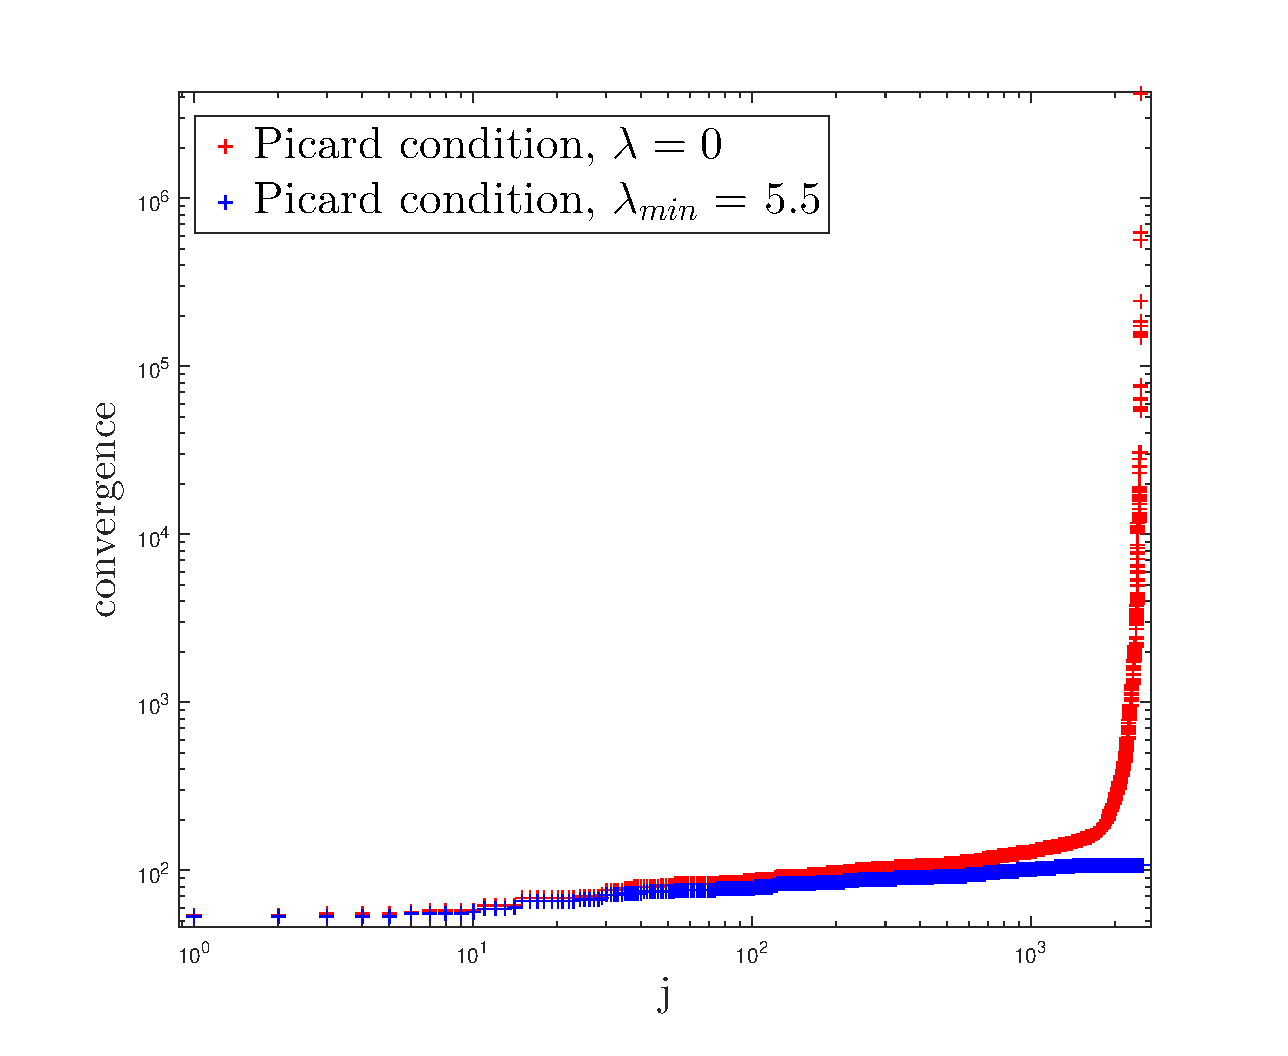
\includegraphics[width=0.5\textwidth]{picardIter.eps} }}
	\end{center}
	\caption{(a) Rekonstruktion durch SWZ, für ein Phantombild $(50\times50)$, Mit der Detektorbreite $k = 50$ und Winkelanzahl $q = 50$. (b) die  Konvergenz der Reihe (\ref{equa:2.4}) blau mit Regularisierung $\lambda_{min} = 5.5$ (das Minimum aus (a)), rot ohne Regularisierung.}
	\label{fig:3.13}
\end{figure}

\begin{figure}[!h]
	\centering
	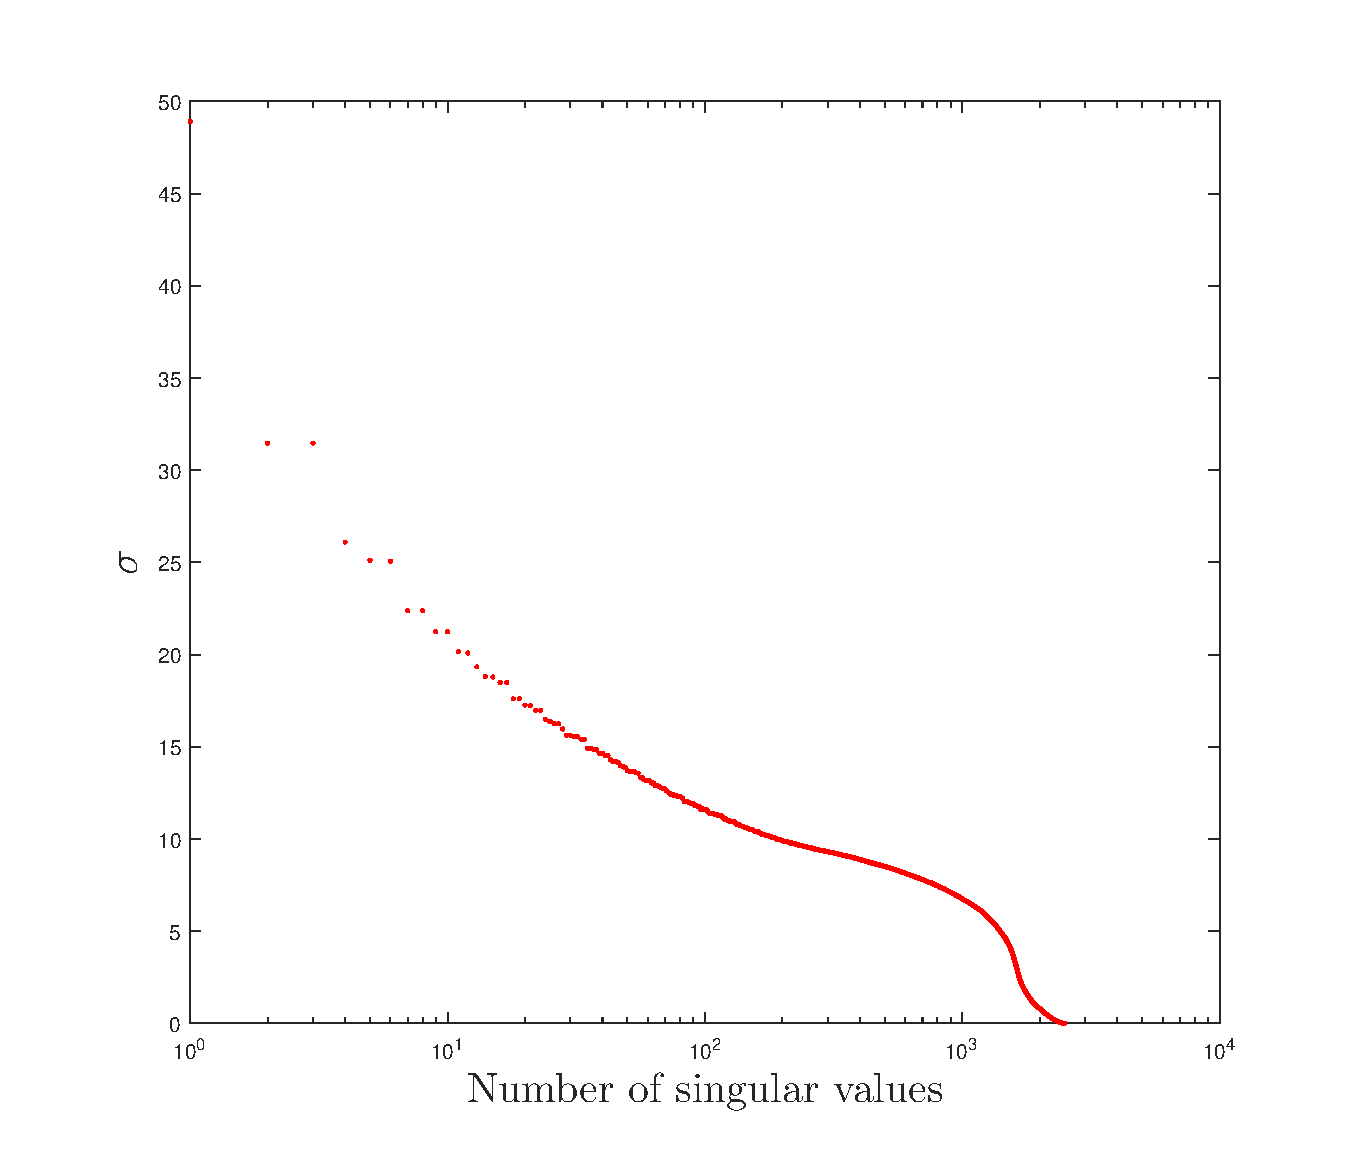
\includegraphics[width=0.5\textwidth]{singVal.eps}
	\caption{Die Folge der Singulärwerte für $A$ aus \ref{fig:3.13.a}}
	\label{fig:3.14}
\end{figure}

Insgesamt zeigt die Abbildung \ref{fig:3.13.b} die Schlechtgestelltheit des hier betrachten Problems $Af = p$ an einem konkreten Beispiel auf. Wir wissen, dass die Pcard-Bedingung (\ref{satz:3}) einen schnellen Abfall der Fourier-Koeffizienten $\langle p, u_i \rangle$ fordert, was eine stabile Lösung garantieren würde. Jedoch ist das bei Kompakten Operatoren, wie $\mathcal{R}$ ist es nie der Fall. Der Grund ist die SWZ, bei der die Singulärwerte eine abfallende Folge bilden (Abb. \ref{fig:3.14}). Was natürlich bei sehr kleinen Singulärwerten die Konvergenz der Reihe nicht fördert. Konvergiert die Reihe nicht, heißt das, dass die gemessenen Projektionen nicht in dem Bild der Operators $\mathcal{R}$ liegen. Was im Falle der verrauschten Daten garantiert ist. Durch eine passende Regularisierung ($\lambda = 5.5$) verschiebt man die verfälschten Fourier-Koeffizienten in die richtige Richtung und bekommt damit eine Minimum-Norm-Lösung. Was hier wieder zu der Abbildung \ref{fig:3.13.a} führt. Die Wirkung der Regularisierung ist in der Abbildung \ref{fig:3.15} offensichtlich.
\begin{figure}[!h]
	\centering
	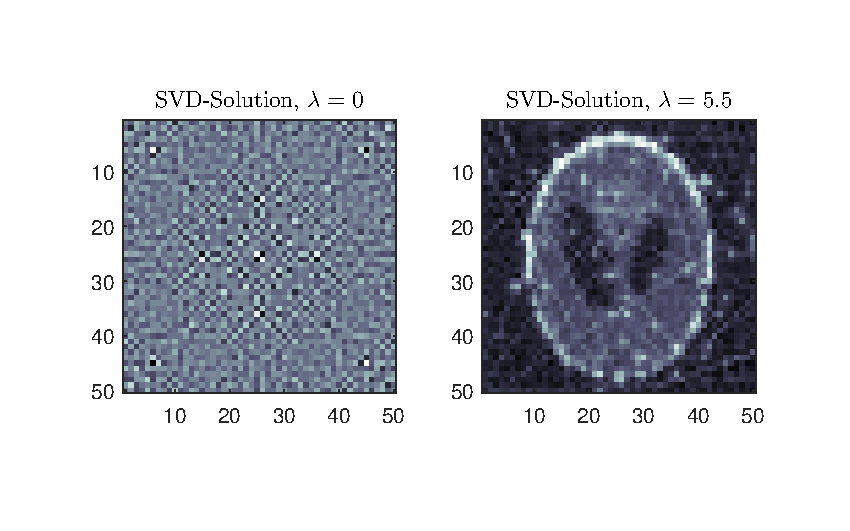
\includegraphics[width=\textwidth]{svdRedANDnotReg.eps}
	\caption{Die Rekonstruktion des Phantombildes mit der Größe $50\times50$ Pixel. Links nicht regularisiert $\lambda = 0$, recht Regularisierung mit $\lambda=5.5$.}
	\label{fig:3.15}
\end{figure}

Es ist natürlich sehr aufwendig, das Verfahren für verschiedene $\lambda$ rechnen zu lassen, um eine Minimum-Norm-Lösung zu bekommen. In der Praxis gibt es ein heuristisches Verfahren mit dem man ein optimales $\lambda_{opt}$ bestimmen kann. In der Abbildung (\ref{fig:3.14}) sehen wir, dass die Folge des Singulärwerte etwa bei $10^3$ einen Knick nach unten macht, die Singulärwerte in diesem Bereich haben den Wert zwischen 4-6. Setzt man diese Werte für $\lambda$ zu Regularisierung ein, so liefert das Verfahren die Minimum-Norm-Lösung.

		%----------------------------------------------------
		% Anhänge
		\appendix
		\chapter{Implementierung}
\label{cha:A}

Hinweise zu konkreten Gegebenheiten, so etwas, wie FEniCS Package und dessen Nichtverfügbarkeit unter Windows, umsomehr die Benutzung des Dockers für diese Zwecke. 
	% Technische Ergänzungen
		\chapter{Inhalte der vollen Masterarbeit}
\label{app:cdrom}

\paragraph{Format:} 
		GitHub Repository: \href{https://github.com/RadmirG/Master-Arbeit}{Radmir Gesler Master Arbeit}


\section{PDF-Dateien}
\begin{itemize}
	\item \href{https://github.com/RadmirG/Master-Arbeit/blob/master/MA_latex/MA_Gesler.pdf}{MA\_Gesler.pdf} - gesamte Masterarbeit im PDF-Format 
\end{itemize}


\section{Python Code}

\begin{itemize}
	
	\item Einzelne Implementierung findet man im Verzeichnis \href{https://github.com/RadmirG/Master-Arbeit/tree/master/code/DeapXDE_heat_equa}{/code/}

\end{itemize}	% Inhalt der CD-ROM/DVD
		%----------------------------------------------------
		\MakeBibliography % Print Bibliography
		\listoffigures % Print the list of figures
		\listoftables % Print the list of tables
\end{document}
%============================================================
